%%%%%%%%%%%%%%%%%%%%%%%%
%% Sample use of the infthesis class to prepare a thesis. This can be used as 
%% a template to produce your own thesis.
%%
%% The title, abstract and so on are taken from Martin Reddy's csthesis class
%% documentation.
%%
%% MEF, October 2002
%%%%%%%%%%%%%%%%%%%%%%%%

%%%%
%% Load the class. Put any options that you want here (see the documentation
%% for the list of options). The following are samples for each type of
%% thesis:
%%
%% Note: you can also specify any of the following options:
%%  logo: put a University of Edinburgh logo onto the title page
%%  frontabs: put the abstract onto the title page
%%  deptreport: produce a title page that fits into a Computer Science
%%      departmental cover [not sure if this actually works]
%%  singlespacing, fullspacing, doublespacing: choose line spacing
%%  oneside, twoside: specify a one-sided or two-sided thesis
%%  10pt, 11pt, 12pt: choose a font size
%%  centrechapter, leftchapter, rightchapter: alignment of chapter headings
%%  sansheadings, normalheadings: headings and captions in sans-serif
%%      (default) or in the same font as the rest of the thesis
%%  [no]listsintoc: put list of figures/tables in table of contents (default:
%%      not)
%%  romanprepages, plainprepages: number the preliminary pages with Roman
%%      numerals (default) or consecutively with the rest of the thesis
%%  parskip: don't indent paragraphs, put a blank line between instead
%%  abbrevs: define a list of useful abbreviations (see documentation)
%%  draft: produce a single-spaced, double-sided thesis with narrow margins
%%
%% For a PhD thesis -- you must also specify a research institute:
%\documentclass[phd,ilcc,twoside]{infthesis}

%% For an MPhil thesis -- also needs an institute
% \documentclass[mphil,ianc]{infthesis}

%% MSc by Research, which also needs an institute
% \documentclass[mscres,irr]{infthesis}

%% Taught MSc -- specify a particular degree instead. If none is specified,
%% "MSc in Informatics" is used.
% \documentclass[msc,cogsci]{infthesis}
 \documentclass[msc, ai, logo, 11pt, twoside, sansheadings]{infthesis}  % for the MSc in Informatics


%% Master of Informatics (5 year degree)
% \documentclass[minf]{infthesis}

%% Undergraduate project -- specify the degree course and project type
%% separately
% \documentclass[bsc]{infthesis}
% \course{Artificial Intelligence and Psychology}
% \project{Fourth Year Project Report}

%% Put any \usepackage commands you want to use right here; the following is 
%% an example:
\usepackage[sort, numbers]{natbib}
\usepackage{url}
%% Information about the title, etc.
\title{BRISK-based Visual Landmark Localisation using Nao Humanoid Robots}
\author{Daniel Mankowitz}


%% If the year of submission is not the current year, uncomment this line and 
%% specify it here:
% \submityear{1785}

%% Optionally, specify the graduation month and year:
% \graduationdate{February 1786}

%% Specify the abstract here.
\abstract{%
This thesis compares five feature extraction algorithms in order to determine the best algorithm to be implemented on a Nao humanoid robot for the purpose of localisation. The immediate application of this method is Robocup. The feature extraction algorithms include BRISK-based algorithms \cite{Leutenegger2011} as well as 1D SURF that has been developed by the \textit{rUNSWift} Robocup team \cite{Anderson}. A novel scoring function has been developed in order to find the optimal parameters for the BRISK and SURF-based feature extraction algorithms. Using these parameters BRISK0 - U-BRISK \cite{Leutenegger2011}, a variation of BRISK, has been utilised, producing the best overall performance of all the algorithms. In the best case scenario it can match image pairs that overlap one another $90\%$ of the time without matching image pairs that do not overlap. This method can match Nao image pairs under varying illumination and can achieve reasonable matching performance when matching Nao images with those captured by a Nikon camera. A key result is that this method has been able to match a Nao's camera images with Google Street View images (albeit with decreased performance) which suggests that street navigation with the Nao may be possible. In addition, two novel geometrical constraints has been developed to remove invalid interest point matches in images. A novel interest point property has also been proposed that may be used for the same purpose. Finally, an addition to the localisation algorithm that is currently used for Robocup has been proposed. This addition will incorporate the BRISK0 U-BRISK feature extraction algorithm into the localisation algorithm. This enables the Nao to efficiently determine its location on the football field.\\
}

%% Now we start with the actual document.
\begin{document}

%% First, the preliminary pages
\begin{preliminary}

%% This creates the title page
\maketitle

%% Acknowledgements
\begin{acknowledgements}
I would like to extend a huge thank you to my supervisor, Dr. Subramanian Ramamoorthy, for his incredibly helpful advice and useful insight that guided me in the right direction, resulting in a successful thesis. In addition I would like to thank Benjamin Rosman for his great advice and useful feedback which were very helpful in developing my thesis. Aris Valtazanos was instrumental in helping me gain an excellent understanding of the Nao robot. Efstathios Vafeias gave me useful insight into the inner-workings of feature extraction algorithms and the Nao's localisation module. I am also really grateful to Stephen McDonagh for his helpful feedback and useful comments.\\
\end{acknowledgements}

%% Next we need to have the declaration.
\standarddeclaration

%% Finally, a dedication (this is optional -- uncomment the following line if
%% you want one).
% \dedication{To my mummy.}

%% Create the table of contents
\tableofcontents

%% If you want a list of figures or tables, uncomment the appropriate line(s)
 \listoffigures
 \listoftables

\end{preliminary}

%%%%%%%%
%% Include your chapter files here. See the sample chapter file for the basic
%% format.

\chapter{Introduction}
\label{sec:introduction}
\section{Motivation}
\label{sec:motivation}
Mobile Robot Localisation is defined as the ability of a mobile robot to determine its pose relative to a map of an environment \citep{Thrun2002}. Localisation is achieved by identifying landmarks in the environment and determining their corresponding positions on the map. The robot then uses this information to determine its pose. If a map of the environment is available, then the robot can immediately orient itself with respect to the map. However, in many cases a map is not available, in which case the robot has to first build a map of the environment and then localise using this map. This is referred to as Simultaneous Localisation and Mapping (SLAM) \citep{Durrant2006, Bailey2006b}.\\

The ability of a robot to localise itself with respect to its environment is crucial in many different applications. One of the more well-known applications is that of the Mar's Rover used for space exploration. Due to a large communication latency, sending commands to the Mar's Rover has a one-way data transfer time that varies between $6$ and $20$ minutes \citep{Powell2006}. Therefore, performing teleoperations to control the rover is impractical and often infeasible. The robot is therefore required to be autonomous which includes the ability to localise itself with respect to its environment such that it can identify landmarks, compute safe traversal paths and avoid obstacles \citep{Powell2006}.\\

Another application where localisation is of great importance is related to the \textit{DARPA Robotics Challenge} \citep{darpa}. The most recent challenge requires the development of robots for disaster-response operations. Often natural and man-made disasters create grave-risks for rescue and aid workers preventing a timely human response. Thus one potential solution is to deploy robots that can build maps and localise themselves in these environments and perform useful tasks such as clearing disaster sites and searching for victims as shown in \figref{fig:darpa} \citep{darpa}.\\   

\begin{figure}[h!] 
  \centering
    \includegraphics[width=0.5\textwidth]{../Drawings/introduction/drcRobots.jpg}
    \caption{An artist's impression of the robots to be developed for the DARPA Robotics Challenge}
    \label{fig:darpa}
\end{figure}

In the past, identification of landmarks for the purposes of localisation and SLAM have been performed with laser-range finders and sonar sensors among others \cite{Davison2007}. Laser-range finder systems are usually accurate but slow whereas sonar sensors are fast and cheap but generate crude measurements \cite{Se2002}. On the other hand, vision perception systems such as cameras are of high resolution and are more intuitive since animals and humans heavily rely on this sense to navigate \cite{Davison2007}. In addition, vision perception systems are inexpensive and ubiquitous and therefore provide a feasible means for a robot to identify landmarks and subsequently localise itself in an environment.\\

Using visual perception to perform localisation is highly desirable in a number of applications. Visual Odometry has been used as a localisation technique on the Mar's Rover \cite{Di2008} but since it requires a large amount of processing time, it can only be used in limited scenarios. This is in spite of the fact that visual odometry provides more accurate position estimation than previously used methods \cite{Powell2006}. Robots deployed to disaster zones can also benefit from visual perception systems for localisation. Here, the robot's ability to distinguish between different sides of a room or building as well as uniquely identifying specific regions within the disaster zone is of great importance in these dynamic environments. In principal, visual perception systems could potentially be used to localise robots that are exploring suburbs and cities. If a robot can uniquely identify visual landmarks whilst in a specific street, then it can in principal determine its location by comparing these visual landmarks to a database of visual landmarks coupled with pre-defined locations. An image database such as Google Street View could be used for this purpose \cite{StreetView}.\\

Performing localisation using a visual perception system faces a number of difficult challenges. The first main challenge is identifying stable visual landmarks that do not vary significantly over time \cite{Davison2007, Se2002}. In addition to this, the same landmarks may be re-observed from different scales, orientations and translations \cite{Szeliski2010}. Thus, depending on the domain, the landmarks need to be invariant to some or all of these changes. Visual landmarks may also suffer from occlusion and varying lighting conditions, which may prevent the landmark from being re-observed. Finally, perhaps the most crucial aspect of visual landmark localisation is that the image processing required to identify the landmarks is computationally expensive. Thus, depending on the system, the technique utilised to identify visual landmarks may need to be adjusted to satisfy the system's computational requirements. \\

\subsection{Application Domain}
\label{sec:domain}
An immediate domain for using a visual perception system to identify landmarks and perform localisation is the Robocup competition. Robocup is a robot football competition that was setup in 1997 in order to advance research in Artificial Intelligence (AI) and Robotics \cite{Robocup}. The original goal of the Robocup competition was to field a team of robots that would be able to defeat the human football world champions by the year $2050$.\\

There are a number of different leagues in which different types of robots compete. The Humanoid Nao robot, which is the robot that will be used for this project, currently competes in the Standard Platform League \cite{StandardPlatform}.\\

The general setup of a Robocup game of football in the Standard Platform League is shown in \figref{fig:naofield}. There are four robots per team which include one goalkeeper and three outfield players \cite{Rules}. The aim of the game is to score more goals than the opponent using a Mylec orange street hockey ball by kicking the ball into the opponent's goal.\\

%Identify common methods applied in the field and voids in literature
\begin{figure}[h!] 
  \centering
    \includegraphics[width=0.8\textwidth]{../Drawings/robocup/NaoField.pdf}
    \caption{The standard setup for a game of football before kick-off \cite{Rules}}
    \label{fig:naofield}
\end{figure}

This year, the Robocup environment has incorporated a significant modification. The goal posts, which were previously yellow and blue for each team respectively, will now be the same colour. This means that the robot will be unable to disambiguate between its side of the field and that of its opponents due to the symmetrical nature of the environment as shown in \figref{fig:naofield}. This makes it difficult for the robot to self-localise itself relative to the field.\\

This recent modification to the Robocup has created the opportunity to determine whether the Nao's visual perception system can be used to identify visual landmarks that are found outside of the field. These landmarks can then be used to localise the Nao's position on the football field. This is a useful domain since many of the problems inherent to disaster zones and the Mars rover are also apparent in the Robocup competition. These include ambiguities due to the symmetrical nature of the environment as well as the dynamics of the environment such as humans and other robots potentially occluding the visual landmarks.\\

\subsection{Nao's Visual Perception System}
\label{sec:naoSpecs}
The Nao robot to be used for the project will use the latest Nao head, Head $4.0$, that has been designed by Aldebaran Robotics \cite{NaoHead}. The specifications for the new Nao head are shown in \figref{fig:nao1} and \figref{fig:nao2} respectively. The Nao's head incorporates a visual perception system that will be used to identify visual landmarks to be used for localisation.\\

The Nao's visual perception system consists of two cameras that are placed vertically above one another. These cameras provide a $640 \times 480$ resolution and operate at $30$ frames per second (fps). These cameras operate in the \textit{YUV422} colour space. Only the upper camera will be used for this project since visual landmarks as high above the field as possible are desired.\\

It is important to note that the Vertical field of view has been increased for each of the cameras respectively to $47.64^\circ$ which may make it possible to detect features on the ceiling above the Robocup field. In addition to this wider field of view, the robot has a yaw range of $-119.5^\circ$ to $119.5^\circ$ and a pitch range of $-38.5^\circ$ to $29.5^\circ$ as shown in \figref{fig:yawPitch}.\\ 

 \begin{figure}[ht!]
\begin{minipage}[b]{0.5\linewidth}
  \centering
    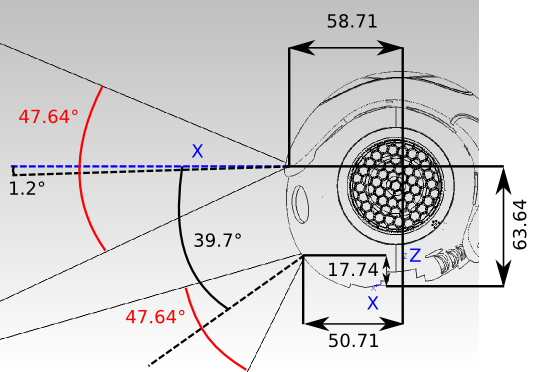
\includegraphics[width=0.6\textwidth]{../Drawings/naoHead/naoHead.jpg}
    \caption{A side view of the new Nao head \cite{NaoHead}} 
    \label{fig:nao1}
\end{minipage}
\begin{minipage}[b]{0.5\linewidth}
  \centering
    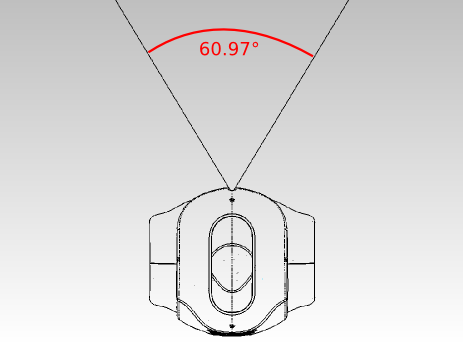
\includegraphics[width=0.6\textwidth]{../Drawings/naoHead/naoHead1.jpg}
    \caption{A top view of the new Nao head \cite{NaoHead}} 
    \label{fig:nao2}
\end{minipage}
\begin{minipage}[b]{0.5\linewidth}
  \centering
    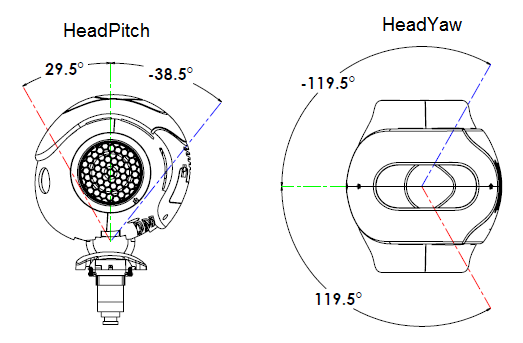
\includegraphics[width=1.0\textwidth]{../Drawings/naoHead/headyawpitch.png}
    \caption{The yaw and pitch of the Nao head \cite{NaoHead}} 
    \label{fig:yawPitch}
\end{minipage}
\end{figure}


%A landmark that has been identified using a visual perception system is often referred to as an \textit{interest point}. One popular definition of an interest point is a specific location or patch in an image that has a large contrast change with respect to its neighbors \cite{Szeliski2010}. Examples include edges and corners in images.\\
\section{Main Objectives}
\label{sec:objectives}
The detection of visual landmarks (also referred to as \textit{Interest Points}) is achieved using feature extraction algorithms. A feature extraction algorithm utilises camera images to extract visual algorithmic-dependant interest points from the environment. These interest points can then be used as landmarks and a robot can then localise itself by subsequently re-observing these landmarks. \\

This thesis conducts a comparison of five different feature extraction algorithms in terms of computational performance and matching accuracy. Matching accuracy refers to the ability of an algorithm to correctly match a pair of images that contain the same visual landmarks. Image datasets are generated using the Nao's upper camera and the algorithms are compared on this data. The algorithm with the best performance along these dimensions is then further analysed and is recommended as the algorithm to be implemented on the Nao robot. In addition to this, a localisation algorithm has been developed for the purpose of Robocup. This algorithm aims to incorporate the best performing feature extraction algorithm to enable the Nao robot to localise itself on the football pitch.\\


%Localisation is where an agent is given a map of the environment and needs to determine its position relative to the map. This can be achieved be forming hypotheses of possible positions and weighting the likelihood of being in a certain position based on observations of the environment. If an agent is removed from the environment (the so-called \textit{kidnapping} problem) then it has to re-establish its position relative to the map. In a symmetrical environment, such as a football field, this can be difficult since the robot can be in a number of possible locations on re-entering the football field. In this case, it may be possible to solve the problem by observing visual natural features that are found above the football field.\\
%
%This is a difficult task since the features may be dynamic as a result of changes in illumination. It is also possible that the robot's visual system may not observe the same features based on its location on the pitch. The robot also has limited processing capabilities and thus processing constraints are placed on the possible algorithms. \\
%
%This problem is important since disambiguating a robot's location in an environment, based on observing distinct visual natural features, can create a generic localisation technique that can be extended to more general situations. These include rescue missions and household chores where a robot's ability to determine its location is crucially based on observing distinct visual natural features. An in-depth description of the proposal for solving this task will be described in the sections to follow.\\ 
%
%What is the problem?
%
%Why is it important?
%
%Why is it difficult?

%What is my hypothesis?

\section{Related Work}
\label{sec:relatedWork}
There are a number of different works that utilise feature extraction algorithms to detect visual landmarks and perform robot localisation. One of the first feature extraction algorithms is called the Scale Invariant Feature Transform (SIFT)\cite{Lowe1999}. This algorithm detects landmarks that are invariant to translation, rotation and image scaling and are thus ideal for a situation where features may be detected from multiple views. A Monte Carlo Localisation algorithm has been implemented using SIFT for feature detection \cite{Gil}. The robot is given a map of the environment and, using stereo vision, is able to find its location in an environment with better accuracy than simply using odometry estimates.\\


SIFT has been implemented on various different SLAM implementations. Using a triclops stereo vision system and detecting visual landmarks using SIFT, a mobile robot has been able to perform homing with good accuracy \cite{Se2001, Se2002}. The visual landmarks detected using SIFT were robustly matched and a consistent 3-Dimensional map was generated. SIFT has also been implemented on a mobile robot, with a stereo camera and odometric sensors, using a FastSLAM algorithm. It achieved very good feature tracking and enabled the robot to estimate its position to within $0.5\%$ to $4\%$ of the total distance travelled \cite{Barfoot2005}.\\

SIFT and a variation of SIFT, called Speeded-Up Robust Features (SURF) \cite{Bay2008}, have been utilised for underwater SLAM \cite{Aulinas2011, Thomas}. The work conducted in \cite{Aulinas} extracts features from underwater images using SURF and matches the features using the SURF matching algorithm. This is performed off-line but results in increased accuracy in the final SLAM estimate.\\

Single camera SLAM, more formally referred to as Monocular SLAM (MonoSLAM), has also been utilised to good effect. Davison \textit{et al.} \cite{Davison2007} uses a single uncontrolled camera as the sole sensor on a mobile robot to actively perform localisation and mapping. The algorithm detects persistent natural features in the environment and is also able to determine the orientation of the features. MonoSLAM has also been implemented on a humanoid robot \cite{Wang2011}. SURF was used as the feature detection technique and visual SLAM was achieved.\\

Regarding the Robocup, one previous work has been developed by the \textit{rUNSWift} Robocup team to enable a Nao robot to localise itself on the Robocup football pitch using visual landmarks \cite{Anderson}. Visual landmarks are detected along a single row of pixels that are computed as a vertical average of a band of pixels above the robot's horizon which is defined in \cite{Bhuman}. In addition, a variation of 2D SURF, called 1D SURF, has been developed to detect and match interest points along this single dimension. 1D SURF is significantly faster than 2D SURF and has been implemented in real-time on the robot.\\






There are a number of algorithms currently available such as the Scale Invariant Feature Transform (SIFT)\cite{Lowe1999}. This algorithm detects features that are invariant to translation, rotation and image scaling and are thus ideal for a situation where features may be detected from multiple views. A far faster yet slightly less robust version of SIFT is Speeded-Up Robust Features (SURF) \cite{Bay2008}. This method maintains good performance compared to SIFT as well as other feature detection techniques \cite{Juan2009} and is ideal for systems that are constrained by the amount of processing power available. Another newer and potentially faster feature detection algorithm is that of Binary Robust Invariant Scalable Keypoints (BRISK) \cite{Leutenegger}. This approach utilises a scale-space FAST-based detector and outperforms the original, unmodified version of SURF by an order of magnitude in the experiments conducted in \cite{Leutenegger}.



%(For both appraoches describe stereo vision or monocular vision solutions)
%SLAM-based approaches




%Localisation-based approaches


%1. What other work has been done involving localisation using natural visual landmarks
%1.1 Start by describing localisation using stereo vision.
%1.2 Then describe localisation using a single camera

%2. What have the rUNSWift team achieved using natural visual landmarks.

%The above-mentioned feature detection techniques are used to detect features in the robot's environment. These features are the observations that are fed into localisation as well as Simultaneous Localisation and Mapping (SLAM) algorithms. The observed features are detected and their range and bearing measured either using stereo vision, involving two or more cameras, or using a single camera and various specialised feature-detection techniques.\\





Single camera SLAM, more formally referred to as Monocular SLAM (MonoSLAM), has also been utilised to good effect. Davison \textit{et al.} \cite{Davison2007} uses a single uncontrolled camera as the sole sensor on a mobile robot to actively perform localisation and mapping. The algorithm detects persistent natural features in the environment and is also able to determine the orientation of the features. MonoSLAM has also been implemented on a humanoid robot \cite{Wang2011}. SURF was used as the feature detection technique and visual SLAM was achieved.\\




\section{Outline}
\label{sec:outline}
The structure of the thesis is as follows: Chapter \ref{sec:background} gives an in-depth overview of the main feature extraction techniques that have been used in this project. This includes 2D SURF and Binary Robust Invariant Scalable Keypoints (BRISK). Chapter \ref{sec:sec:realtimeFeatureExtraction} discusses the variations of these methods that have been developed for the purposes of Robocup. This Chapter also includes a discussion of the \textit{rUNSWift} team's 1D SURF feature extraction algorithm. Chapter \ref{sec:matching} details the matching techniques and constraints that have been implemented and developed respectively to match interest points in corresponding images. This is followed in Chapter \ref{sec:localisation} by a description the localisation algorithm that has been developed for the Nao Robot to use in the Robocup competition. Chapter \ref{sec:experimentsResults} contains the results obtained from comparing the various feature extraction algorithms in a number of different environments. The best performing algorithm is then recommended and analysed further. Finally, Chapter \ref{sec:discussionConclusion} concludes the thesis by discussing potential problems, limitations and recommendations for future work. The key results are also summarised.\\
\chapter{Background}
\label{sec:background}

\section{General Feature Extraction Algorithms}
\label{sec:genFeatureExtract}
This chapter describes two feature extraction algorithms, 2D SURF and BRISK, on which the algorithms used for this thesis are based. From here on in, \textit{Detector} will refer to the module of the feature extraction algorithm that is used to detect the interest points. \textit{Descriptor} will refer to the module of the feature extraction algorithm that computes the descriptor for each interest point.\\


\subsection{2D SURF}
\label{sec:2dsurf}
The SURF feature extraction algorithm is based on approximating the Hessian matrix at every point in an image. The determinant of the Hessian is then computed at each point and is referred to as the blob response. This computation is performed over a number of different scales in scale space as well as in image space in order to find local maxima. A non-maximal suppression is then performed and the local maxima that exist after this stage will be defined as interest points. Each interest point is represented by a descriptor of length $64$. Interest points in different images are then matched based on the Euclidean distance between their respective feature vectors. The smaller the distance, the more certain the match becomes. 

\subsubsection{Integral Images}
\label{sec:integralImages}
One of the big advantages in SURF over SIFT \citep{Lowe2004} is its computational efficiency. One of the important tools that are utilised in order to create this advantage in computation is called the Integral Image \citep{Bay2008}. An integral image computes the integral image value $I_{int}(x,y)$ for pixel location $(x,y)$  as a sum of all pixel intensities found to the left and below the current pixel location until the origin. This is presented in \eqnref{eqn:integralImage}. The variable $I(x,y)$ is the individual pixel intensity at location $(x,y)$. Thus the value of each pixel can be interpreted as the area of the rectangle formed from the current pixel to the image origin. It is assumed that the image origin is in the top left corner of the image. \\

\begin{equation}
I_{int}(x,y) = \sum_{i=0}^{i \leq x}\sum_{j=0}^{j \leq y}I(x,y)
\label{eqn:integralImage}
\end{equation}

By computing the integral image, it is possible to reduce the calculation of any upright rectangular image to four operations. This is very useful when computing box filter convolutions that will be described in the sections to follow.\\

\subsubsection{Detector}
\label{2dsurfdetect}
The SURF detector is based on computing the determinant of the Hessian matrix. The Hessian matrix is a matrix of second order partial derivatives and, when calculated for an intensity image   $I(x,y)$, it is of the form shown in \eqnref{eqn:hessian}.\\

\begin{equation}
Hessian = \left[ \begin{array}{cc} \frac{\partial I}{\partial x^2} & \frac{\partial I}{\partial x^2}\\
					    \frac{\partial I}{\partial x^2} & \frac{\partial I}{\partial x^2}\end{array} \right]
\label{eqn:hessian}
\end{equation}

The Hessian matrix is computed in order to identify local maxima and minima in the image. This is achieved by first computing the determinant, also know as the discriminant, of the Hessian matrix. The determinant of the Hessian is shown in \eqnref{eqn:determinant}. If the determinant of the Hessian is negative then a local extremum has not been identified. If the determinant is positive then a local extremum has been identified \citep{Evans2009}. \\

\begin{equation}
det\mid H \mid = \frac{\partial I}{\partial x^2} \frac{\partial I}{\partial y^2} - (\frac{\partial I}{\partial x \partial y})^2
\label{eqn:determinant}
\end{equation}

For a SURF detector, the Hessian is computed for a point $\textbf{x} = (x,y)$ in the Image $I$. The Hessian is computed over multiple scales, $\sigma$, and therefore the Hessian matrix at a point for a specific scale is represented as $H(\textbf{x}, \sigma)$ \citep{Lowe2004} and is defined as shown in \eqnref{eqn:hessianScale}.\\


\begin{equation}
H(\textbf{x}, \sigma) = \left[ \begin{array}{cc} L_{xx}(\textbf{x}, \sigma) & L_{xy}(\textbf{x}, \sigma)\\
					    L_{xy}(\textbf{x}, \sigma) & L_{yy}(\textbf{x}, \sigma)\end{array} \right]
\label{eqn:hessianScale}
\end{equation}

The variable $L_{xx}(\textbf{x}, \sigma)$ is analogous to the second order derivative, $ \frac{\partial I}{\partial x^2}$, detailed in \eqnref{eqn:hessian}. This second order derivative is computed in SURF detectors by convolving the image, at point $\textbf{x}$, with a particular kernel \citep{Evans2009}. The kernel in this instance is the second order Gaussian derivative, $\frac{\partial g(\sigma)}{\partial x^2)}$. \\

There are a number of reasons why Gaussians are used as the kernel in computing the second order derivatives. One of the main reasons is that it is possible to vary the amount of smoothing resulting from the convolution of the Gaussian with the image \citep{Evans2009}. This enables the calculation of the Hessian determinant at different scales which is used for non-maximal suppression and identifying scale-invariant interest points.\\

The SURF implementation approximates Gaussian second order derivatives for the convolution stage by using box filters. Box filters are used to perform very fast convolutions. A box filter consists of positive and negative lobes. Each lobe is assigned a particular weighting. For example, in \figref{fig:boxFilters} \citep{Bay2008}, the white lobes are assigned a weighting of positive one, the black lobes are assigned a weighting of negative one and the gray lobes are assigned a weighting of zero. The box filters are created in the $x$, $y$ and $xy$ directions in order to compute the Hessian and subsequently its determinant. One of the key advantages to this approach is the computational cost. This is because it is possible to use a combination of integral images and box filters to perform the second order derivative computation very efficiently. It is also possible to increase the size of the box filters at no additional computational cost \citep{Bay2008}.\\

\begin{figure}[h!] 
  \centering
    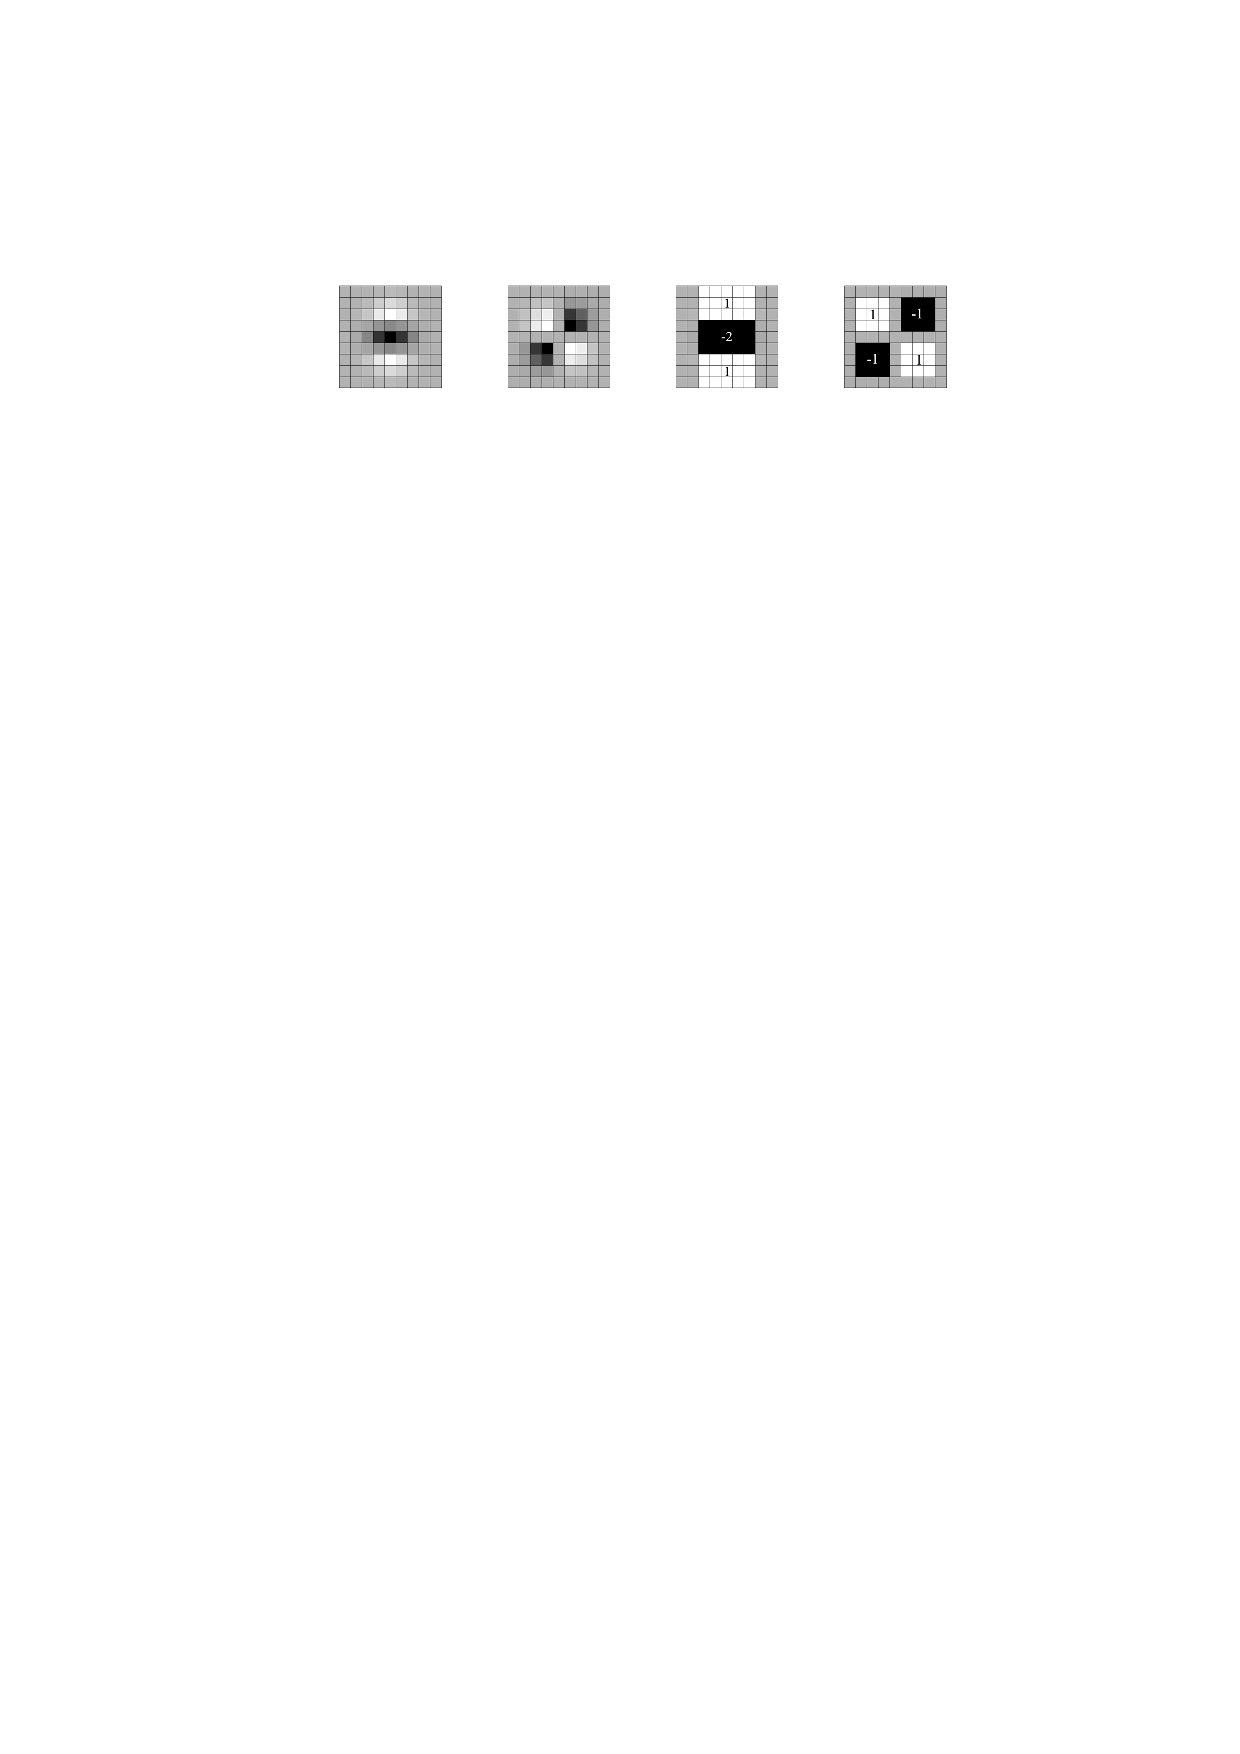
\includegraphics[width=0.8\textwidth]{../Drawings/methods/SURF2D_BoxFilters.pdf}
    \caption{The Box filters used to perform the 2D convolutions}
    \label{fig:boxFilters}
\end{figure}

Therefore, utilising box filters, the determinant of the Hessian is computed as shown in \eqnref{eqn:approxHessian}. The variables $D_{xx}$, $D_{xy}$ and $D_{yy}$ represent the box filter convolutions in the $x$, $xy$ and $y$ directions respectively at a point $\textbf{x} = (x,y)$ in the image $I$.\\ 

\begin{equation}
det \mid H_{approx} (x,y) \mid = D_{xx}D_{yy} - (0.9 D_{xy}^2)
\label{eqn:approxHessian}
\end{equation}

The determinant of the Hessian at a point $\textbf{x} = (x,y)$ in the image $I$ is referred to as the blob response at a scale $\sigma$ \citep{Bay2008}. The blob response is computed at every location in the image in order to create a blob response map. A blob response map exists for every considered scale and these maps are used to detect local maxima in the images.\\

The different scales collectively define the scale space. The scale space can be seen as a function that is used to find extrema across a set of predefined scales. A set of scales is important as interest points need to be found across a number of scales in order to verify that the point is indeed an interest point. It also ensures that the point can be detected at different scales (I.e. points of view).\\

In the SIFT method \citep{Lowe2004}, in order to construct the scale space, an image is convolved with a Gaussian kernel. The image is then sub-sampled and re-convolved with the same kernel to create a new scale. In the SURF method, as mentioned previously, the box filter size can be increased at no computational cost due to the use of integral images. Thus it makes sense to construct the scale space by convolving the image with the box filters, but instead of sub-sampling the image, the box filters can be increased in size and convolved with the same image at very little computational cost. This creates a very efficient `inverted' scale space pyramid as shown in \figref{fig:scaleSpace} \citep{Evans2009}. The higher the position in the pyramid, the larger the scale and vice versa. \\

\begin{figure}[h!] 
  \centering
    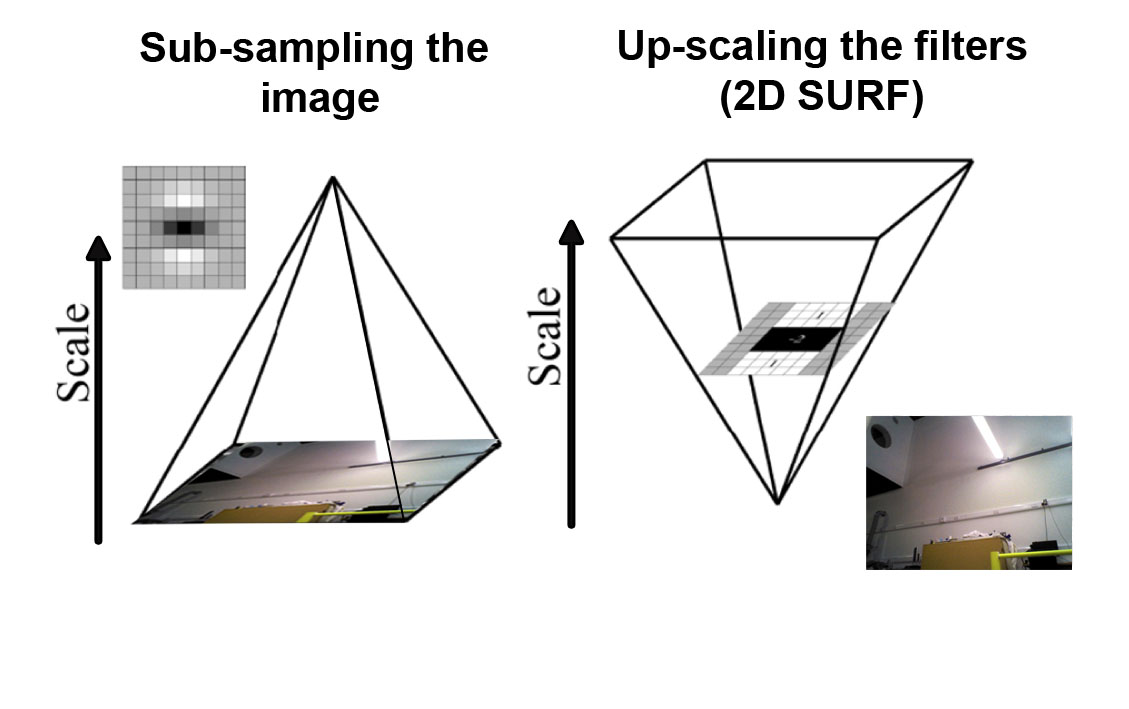
\includegraphics[width=0.8\textwidth]{../Drawings/methods/SURF2D_Image_pyramid.jpg}
    \caption{The up-scaling of the filters is used in 2D SURF rather than the down-scaling of the image}
    \label{fig:scaleSpace}
\end{figure}

The scale space is divided into octaves. An octave consists of a set of blob response maps each resulting from a convolution of the image with a box filter of a specific size. The blob response map corresponding to the lowest level (i.e. smallest scale) of the scale space is constructed using a $9 \times 9$ box filter. This corresponds to a scale value of $1.2$. As the size of the filters used for convolution increase, so too does the scale. During the convolution procedure, the filter is centered on each $(x,y)$ location in the image and each lobe in the filter has a specific width represented by $l_0$. In order to increase the size of the filter (I.e. move up a level in scale space), the filter lobe width, $l_0$, is increased by $2$ pixels. This ensures that the center pixel is still found in the center of the filter. Thus, the first filter is $9 \times 9$ and the next successive filter is $15 \times 15$. \\

The number of octaves used to find interest points depends on the size of the image. Usually, three to four octaves are used. The first octave uses box filters of size $9 \times 9$, $15 \times 15$, $21 \times 21$ and $27 \times 27$ to convolve with the current image.  For each subsequent octave, the filter size increase is doubled. Therefore, for example, the second octave will have filter sizes of $15 \times 15$, $27 \times 27$, $39 \times 39$ and $51 \times 51$ respectively. This corresponds to a filter increase of $12$ pixels. The next octave will have an increase of $24$ pixels and so on \citep{Bay2008}. \\

As mentioned previously, the convolution of the box filters of various sizes produces blob response maps at various scales. The next step involves using the blob response maps to detect interest points at these different scales. The first step in detecting interest points is removing pixels whose blob responses are below a certain threshold. Once the relevant pixels have been thresholded,  a non-maximal suppression is performed in a $3 \times 3 \times 3$ neighborhood surrounding the current pixel. Thus for each octave and each scale within the octave, each pixel is compared to its $26$ neighbors \citep{Evans2009}. This includes its $8$ adjacent neighbors in image space as well as its $9$ neighbors in the scale above and scale below the current image space respectively as shown in \figref{fig:imageSpace} \citep{Lowe2004}. It should be noted that the largest scale and smallest scale for each octave have no scale space layers above or below respectively. Therefore these blob response maps are only used for comparison for the internal scale space layers. \\

\begin{figure}[h!] 
  \centering
    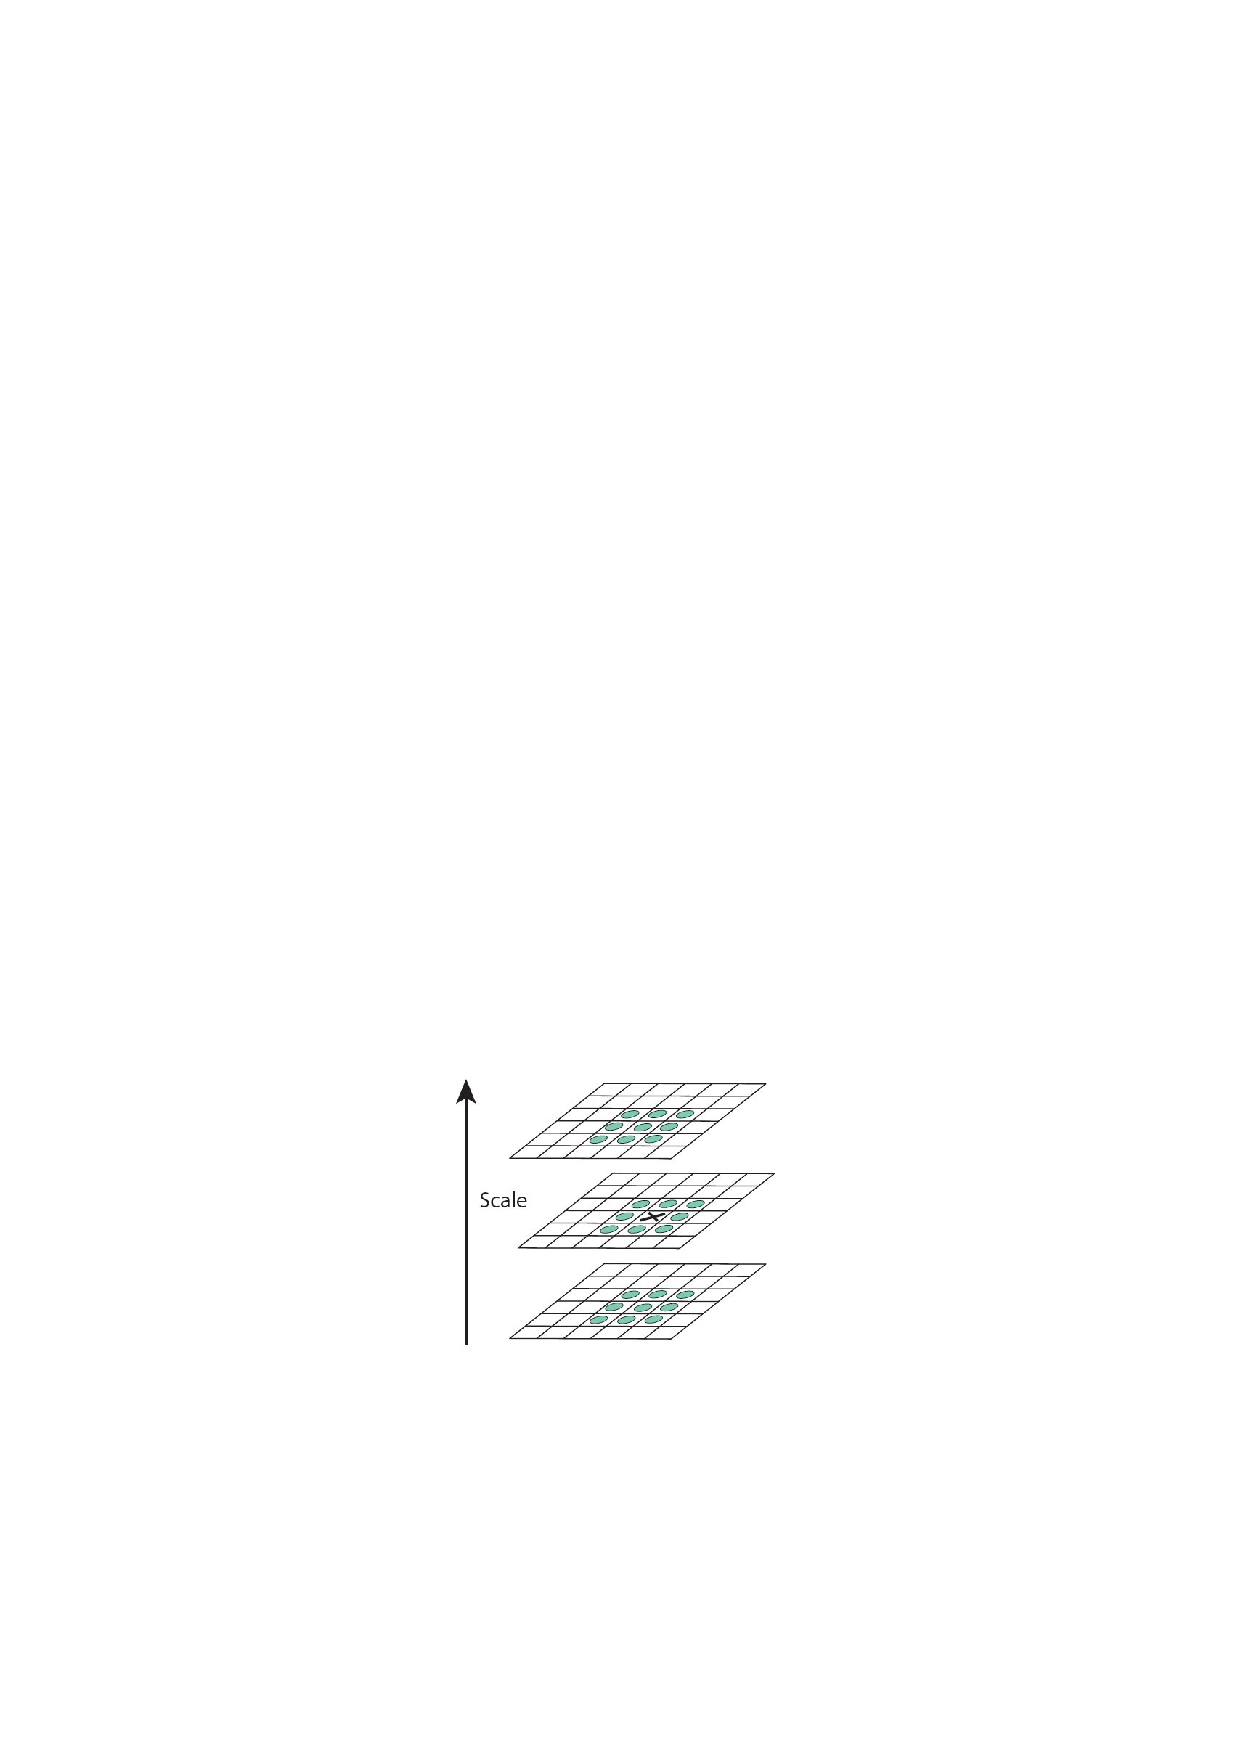
\includegraphics[width=0.5\textwidth]{../Drawings/methods/SURF2D_Nonmaximal_suppression.pdf}
    \caption{The non-maximal suppression performed on each point and its $26$ surrounding neighbors}
    \label{fig:imageSpace}
\end{figure}

If the pixel is not suppressed, then its image space and scale space locations are calculated to sub-pixel accuracy using a linear interpolation procedure \citep{Evans2009}. The pixel becomes an interest point and its descriptor then needs to be determined.\\

%The interpolation procedure TO DO Maybe...

\subsubsection{Descriptor}
\label{sec:2dsurfdescribe}
The SURF descriptor is a $64$ length vector that contains information about the intensity content of the neighborhood surrounding the interest point. In developing the descriptor, a number of important steps need to be implemented. The first step is creating a reproducable orientation for the interest point \citep{Bay2008}. If the interest point is detected at a scale, $\sigma$, then Haar Wavelets of size $4\sigma$ are used to calculate Haar Wavelet Responses (HWRs) for all pixels within a circular radius of $6\sigma$ from the detected interest point.  Haar Wavelets are simple filters that are used in SURF to calculate gradients in the $x$ and $y$ directions respectively. Examples of these wavelets are shown in \figref{fig:haar} \citep{Evans2009}. Once the HWRs have been calculated, they are then weighted by a Gaussian whose mean is centered on the interest point. This means that the pixels found further away from the interest point have a smaller influence on the reproducible interest point orientation.\\


\begin{figure}[h!] 
  \centering
    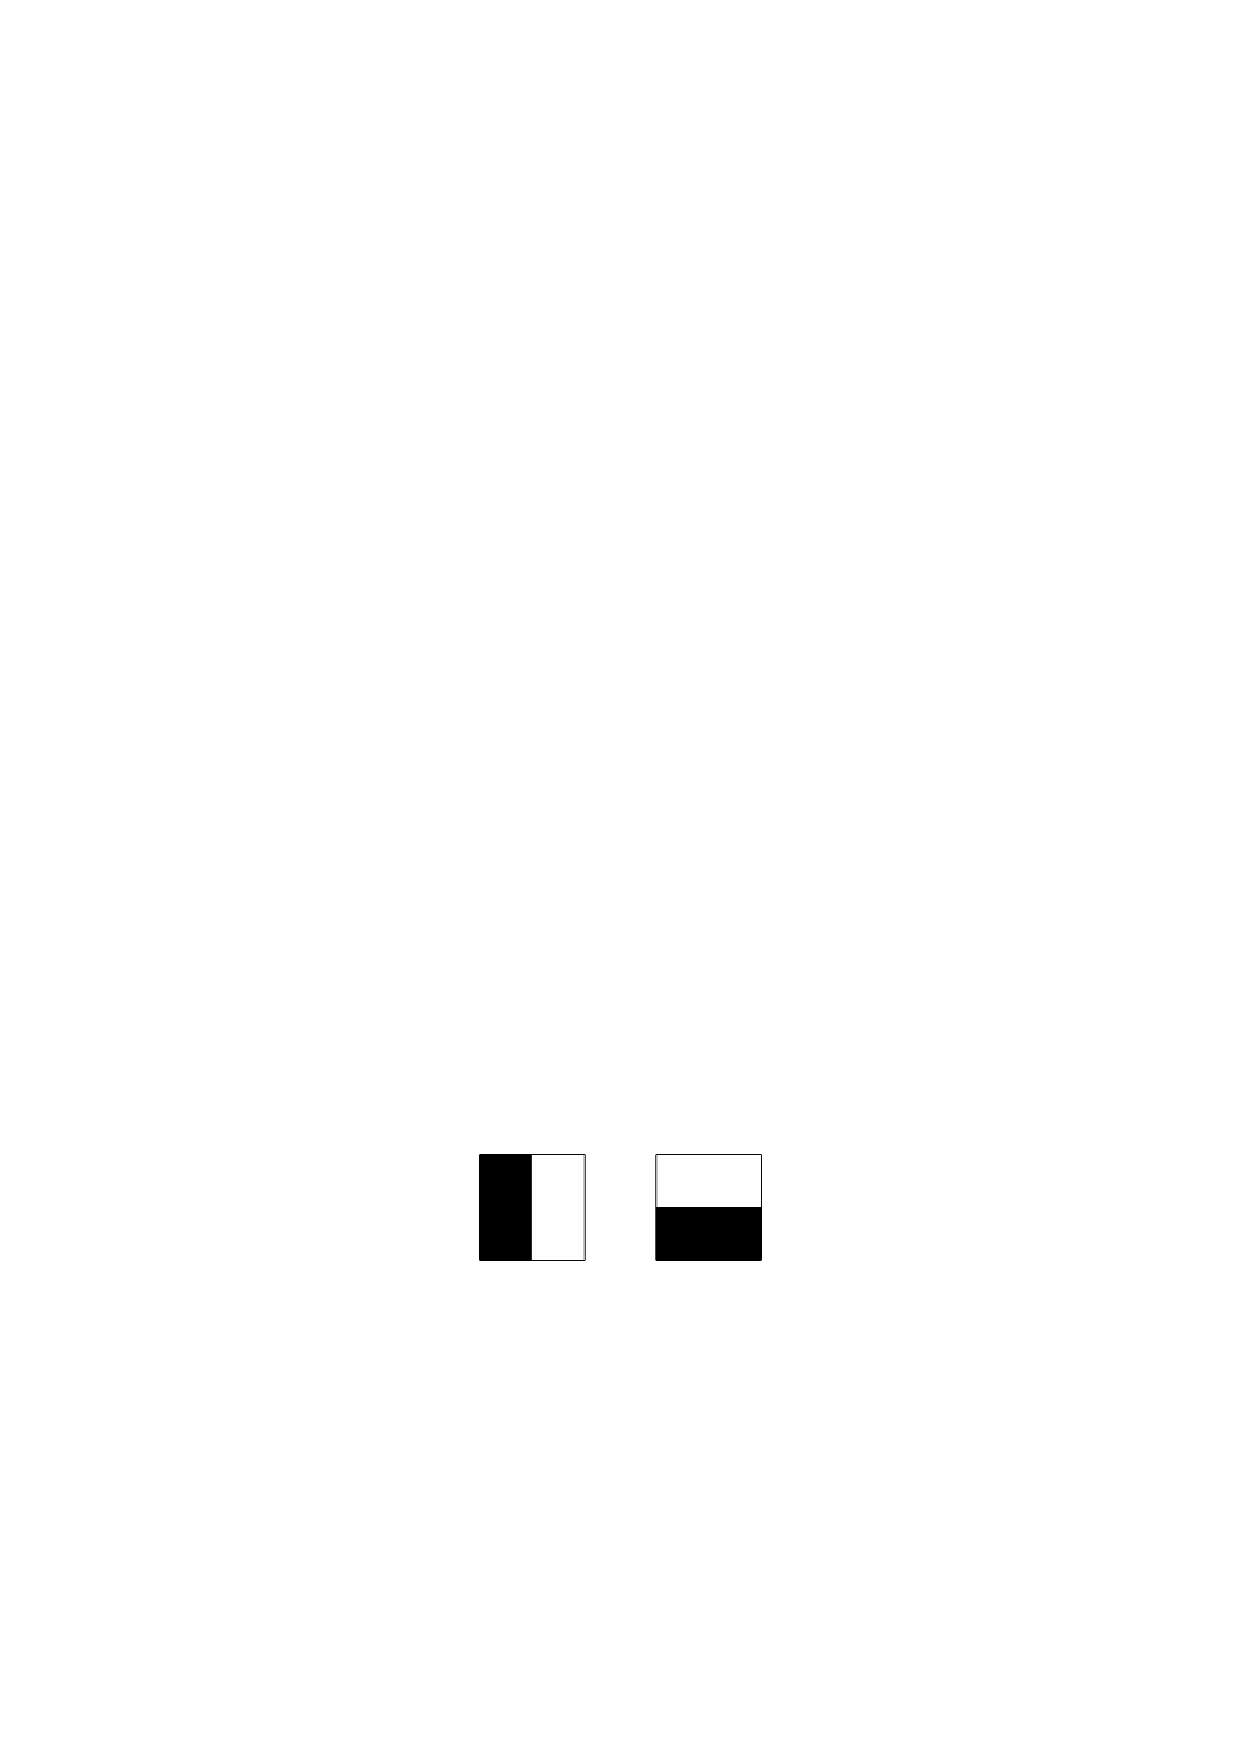
\includegraphics[width=0.5\textwidth]{../Drawings/methods/SURF2D_HaarWavelets.pdf}
    \caption{Haar Wavelets used to calculate the Haar Wavelet Responses. The left Haar Wavelet calculates the responses in the $x$ direction and the right one calculates the Haar Wavelets in the $y$ direction}
    \label{fig:haar}
\end{figure}

In order to find the reproducible orientation, a circular segment of width $\frac{\pi}{3}$ is rotated around the interest point and the HWRs in the $x$ and $y$ directions, within this circular segment, are calculated to yield a vector for that particular circular segment as shown in \figref{fig:circularSegment} \citep{Evans2009}. The longest vector resulting from the rotation of this circular segment around the interest point is assigned to the interest point as the reproducible orientation.\\

\begin{figure}[h!] 
  \centering
    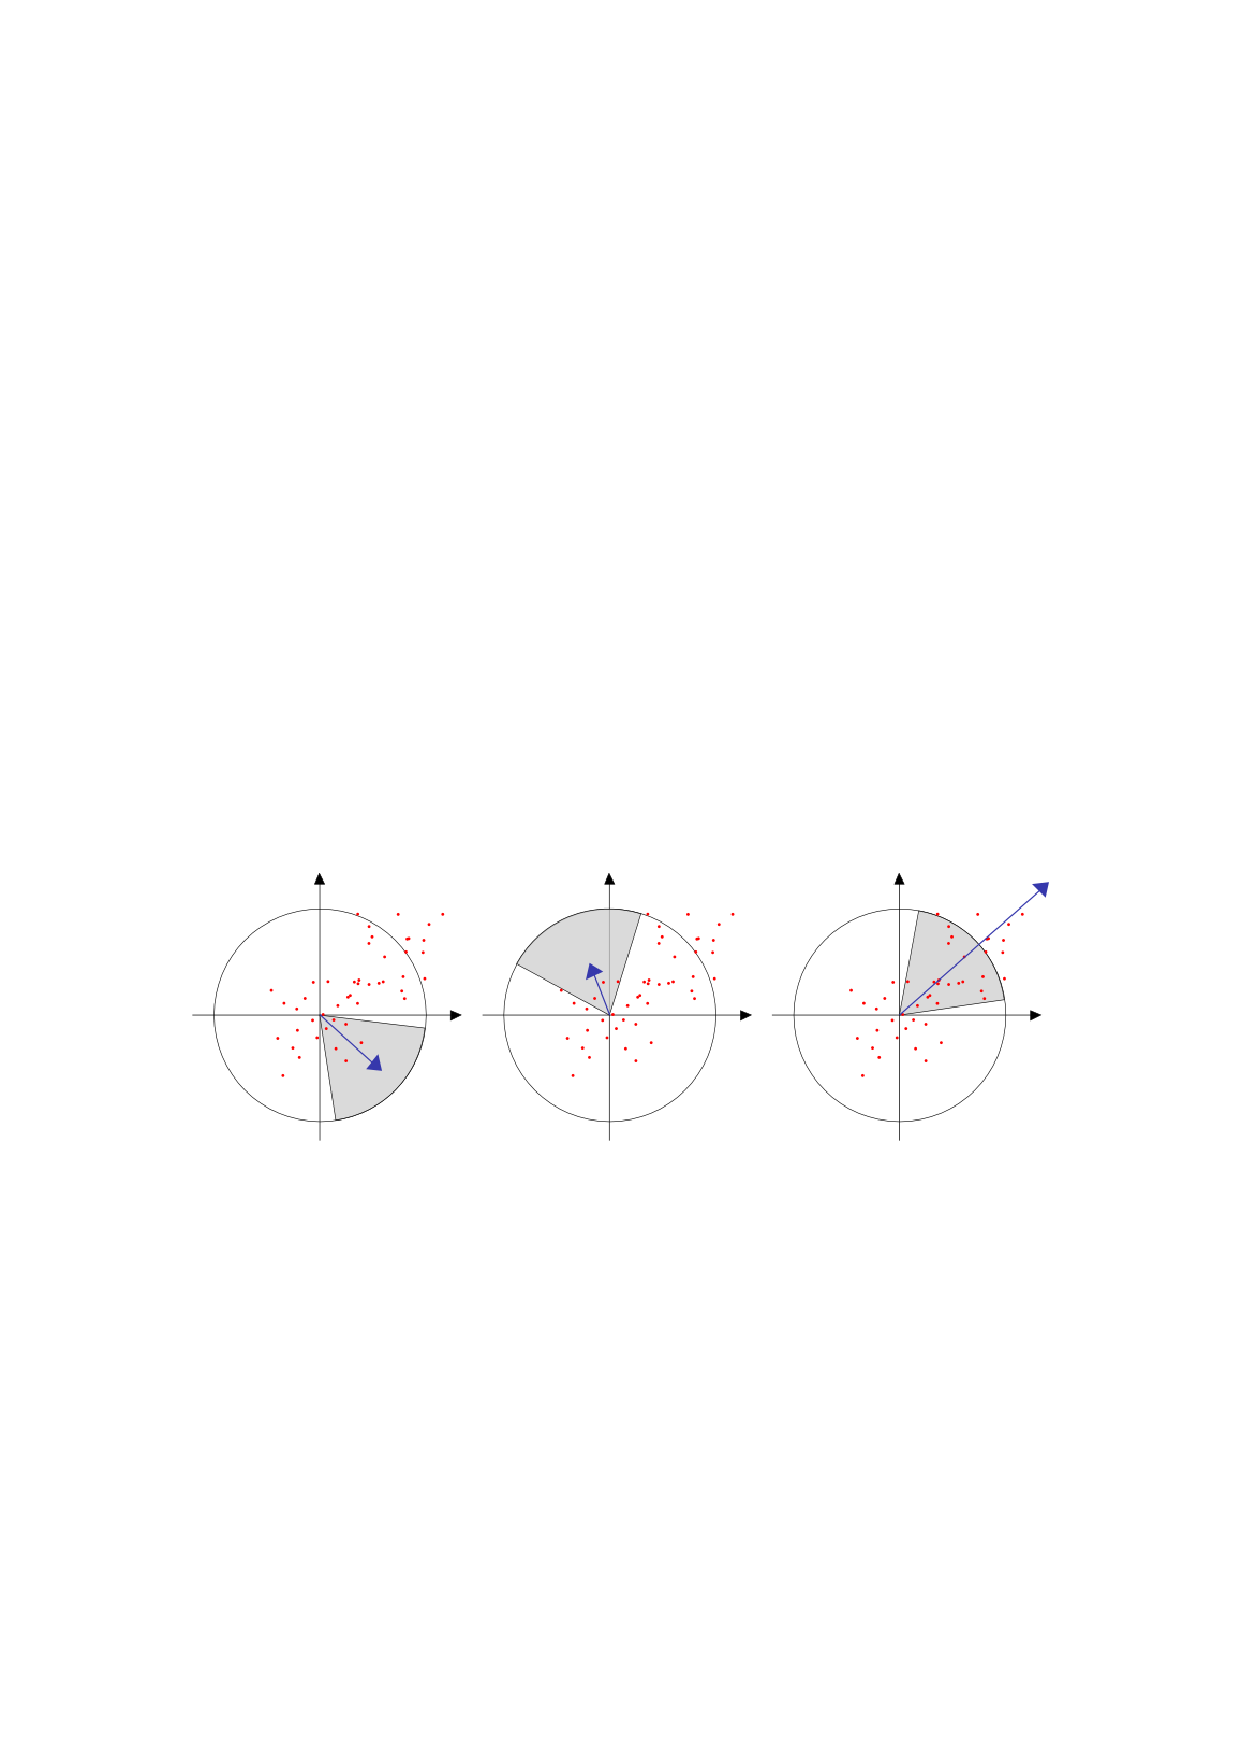
\includegraphics[width=1.0\textwidth]{../Drawings/methods/SURF2D_orientation_assignment.pdf}
    \caption{The $\frac{\pi}{3}$ circular segment calculating the Haar Wavelet Responses for a particular interest point. Here, the right-most figure contains the largest vector and the interest point is therefore assigned the orientation of this vector}
    \label{fig:circularSegment}
\end{figure}

Once the orientation of the interest point has been determined, a square window of size $20\sigma$ is centered around the interest point and is oriented in the direction of the reproducible orientation of that interest point. This square region is then split into $16$ sub-regions of equal size. In each sub-region, HWRs in the $x$ and $y$ directions are then computed for $5 \times 5$ regularly spaced sample points. It is important to note that the $x$ and $y$ directions are relative to the reproducible orientation axes as shown in \figref{fig:reproducibleAxes} \citep{Evans2009}. The HWRs for these $25$ sample points are then summed together to yield the descriptor for the sub-region as shown in \eqnref{eqn:descriptorSub}. Since there are $16$ of these sub-regions, a $64$ length descriptor is created.\\

\begin{figure}[h!] 
  \centering
    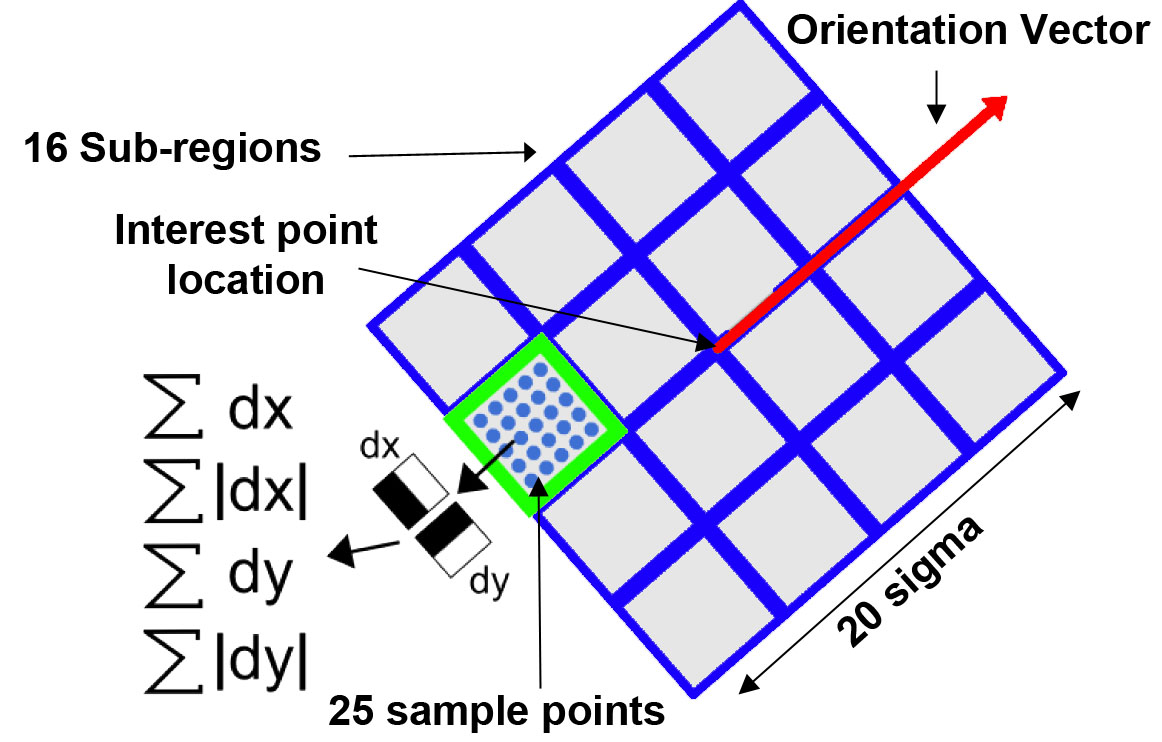
\includegraphics[width=0.5\textwidth]{../Drawings/methods/SURF2D_Descriptor.jpg}
    \caption{The square window centered on the interest point and aligned with the orientation vector}
    \label{fig:reproducibleAxes}
\end{figure}

\begin{equation}
descriptor_{sub} = [\Sigma d_x, \Sigma d_y,  \Sigma \mid d_x \mid , \Sigma \mid d_y \mid] 
\label{eqn:descriptorSub}
\end{equation} 



\subsection{BRISK}
\label{sec:brisk}
A new method has been developed that, in a variety of domains yields performance that betters SURF by an order of magnitude. This method is called Binary Robust Invariant Scalable Keypoints (BRISK) \citep{Leutenegger2011}. This method utilises a technique called Adapative and Generic Corner Detection Based on the Accelerated Segment Test (AGAST) in order to compute a score for a pixel in location $(x,y)$ in image $I$ \citep{Mair2010}. AGAST is largely based on the Features from Accelerated Segment Test (FAST) \citep{Rosten2006} method but incorporates some improvements such as adaptive tree switching which will be briefly discussed. Using this score, interest points are defined. A binary feature descriptor of length $512$ is then generated for each interest point as a result of some simple brightness comparison tests. Interest points are then matched in different images by computing the Hamming distance between the feature descriptors. \\

\subsubsection{FAST Score}
\label{sec:fastScore}

The FAST score, denoted as $s$, is the first criterion that is used in BRISK in order to identify interest points \citep{Rosten2006}. The FAST score is computed by initially choosing a set of $16$ pixels that form a circle centered on the current pixel $p$. $p$ is the potential interest point that is being evaluated, as shown in \figref{fig:fastScore} \citep{Rosten2006}. The circle has a Bresenham radius of $3.4$ pixels \citep{Mair2010}. In order for the pixel $p$ to be considered an interest point, there has to be a set of $n$ (in this case $9$) contiguous pixels from the circle of $16$ pixels that are brighter than the current pixel intensity, $I_p$, plus some threshold $t$, or are darker than $I_p - t$. A larger value of $t$ will reduce the amount of interest points that will be detected. However, these detected points will be strong, salient interest points. \\

\begin{figure}[h!] 
  \centering
    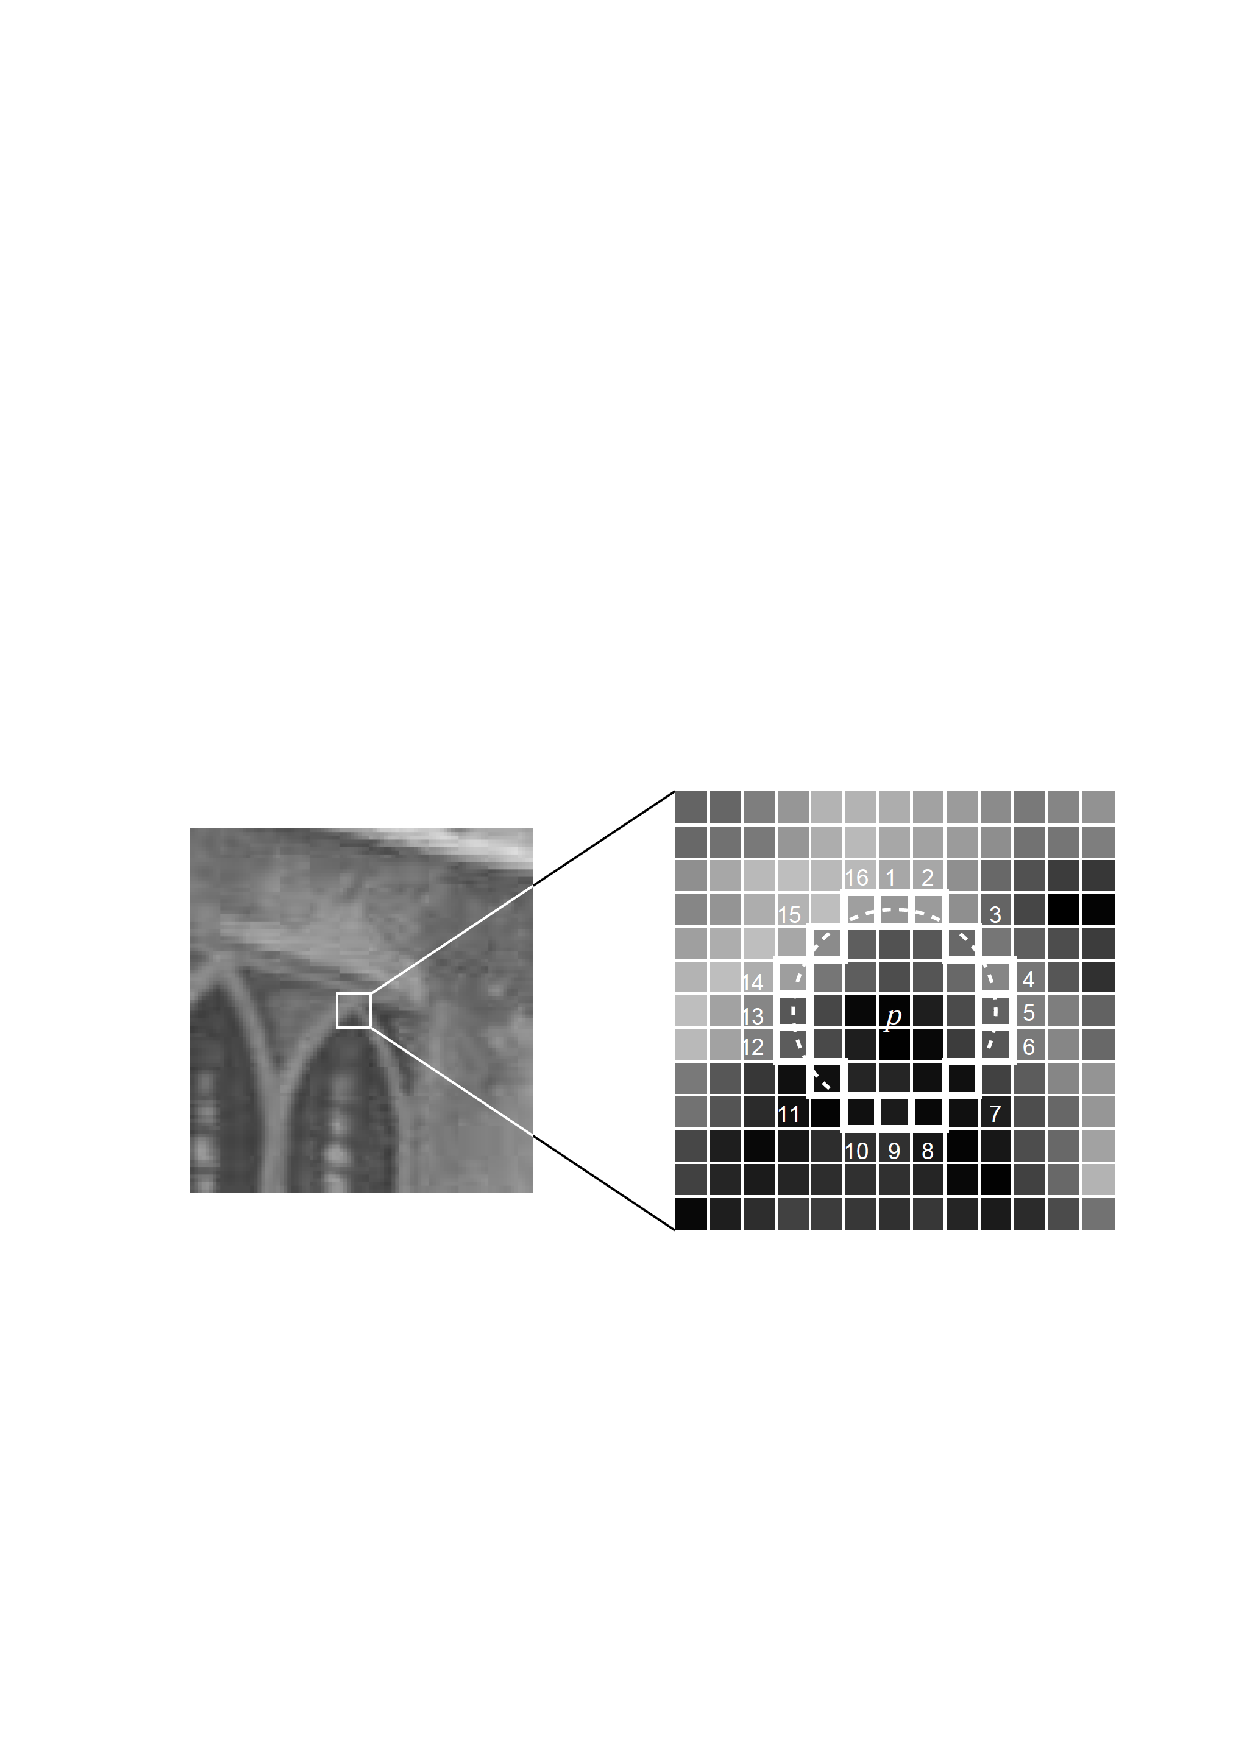
\includegraphics[width=0.8\textwidth]{../Drawings/methods/FASTScoreCalculation.pdf}
    \caption{The calculation of the FAST score for BRISK}
    \label{fig:fastScore}
\end{figure}

The FAST score is computed as the sum of the absolute difference between the circle of pixels and the central pixel. More formally it is expressed as shown in \eqnref{eqn:fastScore}. The variable $I_p$ is the intensity of the central pixel $p$. $I_{p \rightarrow x}$ is the intensity of the pixel at location $x$ on the circle of pixels relative to $p$. $S_{dark}$ refers to all the pixels that are darker than $I_p - t$, whereas $S_{bright}$ refers to all the pixels on the circle that are brighter than $I_p + t$. Taking the maximum of these two quantities yields the FAST score that is used for comparison in determining whether or not the pixel $p$ is an interest point.\\

\begin{equation}
V = max(\sum_{x \epsilon S_{bright}} \mid I_{p \rightarrow x} - I_p \mid - t, \sum_{x \epsilon S_{dark}} \mid I_p - I_{p \rightarrow x} \mid - t)
\label{eqn:fastScore}
\end{equation}

It is important to consider the order in which the points on the circle surrounding the potential interest point are evaluated, for computational efficiency. One method is to evaluate pixels $1, 5, 9 $ and $13$ corresponding to the compass directions \citep{Rosten2006}. At least three of these pixels need to be brighter or darker than the central pixel $p$ plus the chosen threshold in order for the central pixel to be evaluated further. If this is not the case, then the pixel $p$ is discarded as it cannot have $9$ contiguous pixels as mentioned previously and is therefore not an interest point. If at least three of the above-mentioned pixels fulfil the criteria, then the Accelerated Segment Test (AST) is applied to the circle of pixels in order to determine whether or not the central pixel is indeed an interest point. There are different ways of applying the AST in order to determine whether or not a point is an interest point. Both FAST and AGAST use decision trees to search the circle of pixels in a specific order so as to maximise the efficiency with which each potential interest point is evaluated. The techniques differ in terms of the order in which the $16$ circle pixels are evaluated. In addition, AGAST has an adaptive tree switching technique which enables the method to switch to different decision trees that are optimised for a particular area of an image. This has an effect on computational efficiency and how well the methods generalise to different domains.   \\

%FAST performs the AST by first learning a \textit{ternary} tree which has possible pixel states of \textit{brighter}, \textit{darker} or \textit{similar}. In building the tree, at each step, all remaining pixels are asked the question whether or not they are \textit{brighter} or \textit{darker} than the central pixel. The pixel with the highest information gain is chosen as the next branch in the tree. Each pixel can have one of four possible states, namely unknown (u), darker(d), brighter(b) or similar(s). Since $16$ pixels are being evaluated in the circle surrounding the central pixel and each of these pixels have four possible states, there are a total of $4^{16}$ possible configurations. \\
%
%AGAST performs a more efficient and generic AST than that of FAST. One improvement in AGAST's method is that it has a richer configuration space. In addition, a \textit{binary} tree is constructed rather than a \textit{ternary} tree. \textbf{TO DO}\\

\subsubsection{Detector}
\label{briskDetect}
BRISK's scale space has a different structure to that of SURF. In this case, the scale space consists of \textit{n} octaves \textit{$c_i$} and \textit{n} intra-octaves \textit{$d_i$} \citep{Leutenegger2011}. The typical number of octaves chosen for BRISK is $n=4$. The intra-octaves are placed between the octaves. A typical ordering would be $c_0, d_0, c_1, d_1, c_2...$. In order to create the octaves, the image is progressively half-sampled by a factor of two. The first octave corresponding to the original image is called $c_0$ and the first intra-octave $d_0$ is generated by down-sampling the original image by a factor of $1.5$. Thereafter, the image is half-sampled by a factor of two. This creates an image pyramid where the lowest layer is the original image and the higher layers are down-sampled versions of the original image.\\

In BRISK, the FAST score $s$ is computed for each pixel $p$, for each octave and intra-octave respectively \citep{Leutenegger2011}. The same threshold $t$ is used throughout. A non-maximal suppression is then performed on each pixel in every octave and intra-octave respectively. In order to determine whether or not the pixel is indeed an interest point, the pixel $p$ firstly needs to be a maxima (in terms of its FAST score) compared to its $8$ adjacent neighbors in image space. The pixel's FAST score is then compared to the layer above and layer below in the image pyramid. Its FAST score has to be a maxima relative to these values as well. In the case of the original image $c_0$, no layer below this layer exists. To account for this problem, only the layer above $c_0$ is compared.\\

Once a pixel with a maximum score has been detected, a sub-pixel refinement is applied to the maximum by fitting a 2D quadratic function in the least squares sense to a $3 \times 3$ score patch surrounding the detected maximum \citep{Leutenegger2011}. A sub-pixel refinement is also applied to $3 \times 3$ patches in the layers directly above and below the detected maximum in order to generate three local maxima. This procedure is followed by a continuous scale refinement in order to determine the true scale of the detected interest point. A 1D parabola is fitted to these three local maxima along the scale axis as shown in \figref{fig:1dparabola} \citep{Leutenegger2011} and the maximum of this parabola determines the true score and scale of the detected corner. Once the scale has been found, the image coordinates need to be re-interpolated to account for the true scale as the scale may not necessarily lie directly on an octave or intra-octave respectively. This creates a scale invariant interest point.\\

\begin{figure}[h!] 
  \centering
    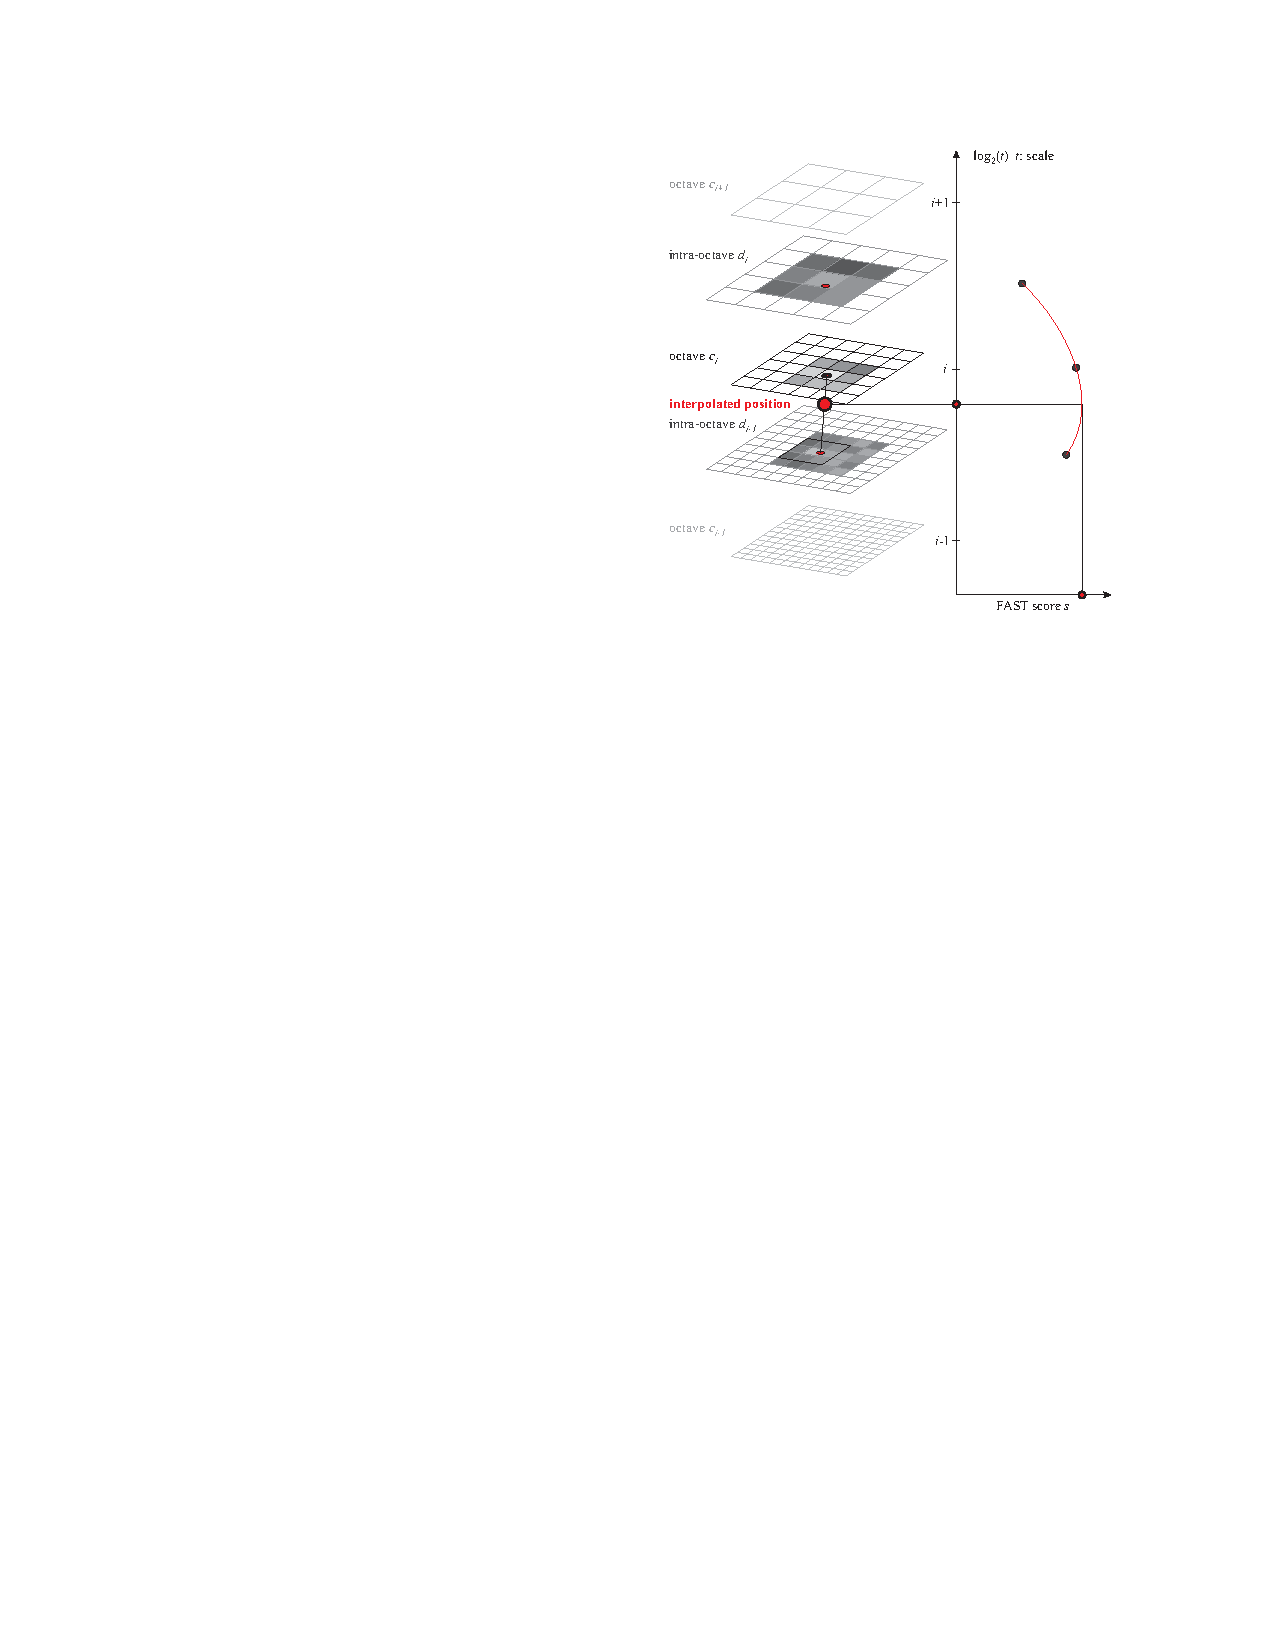
\includegraphics[width=0.8\textwidth]{../Drawings/methods/BRISKScaleSpace.pdf}
    \caption{Sub-pixel refinement and scale refinement is performed by interpolating a 1D parabola along three separate scales}
    \label{fig:1dparabola}
\end{figure}

This procedure is performed on all detected maxima and this produces a set of interest points with sub-pixel refined image locations as well as true scale values. The descriptors for these interest points are subsequently determined.

\subsubsection{Descriptor}
\label{sec:briskDescribe}
One of the important aspects of the BRISK descriptor is that it uses a pre-determined pattern to sample the neighborhood surrounding each detected interest point $k$. Equally spaced samples, $p_i$ are chosen which are placed on concentric circles centered on the interest point. This is shown in \figref{fig:samplingPattern} \citep{Leutenegger2011}. Aliasing can occur and in order to prevent this problem, Gaussian smoothing is applied to each sampled point on the concentric circles with standard deviation $\sigma_i$ proportional to the difference between the sampled points on the circle. \\

\begin{figure}[h!] 
  \centering
    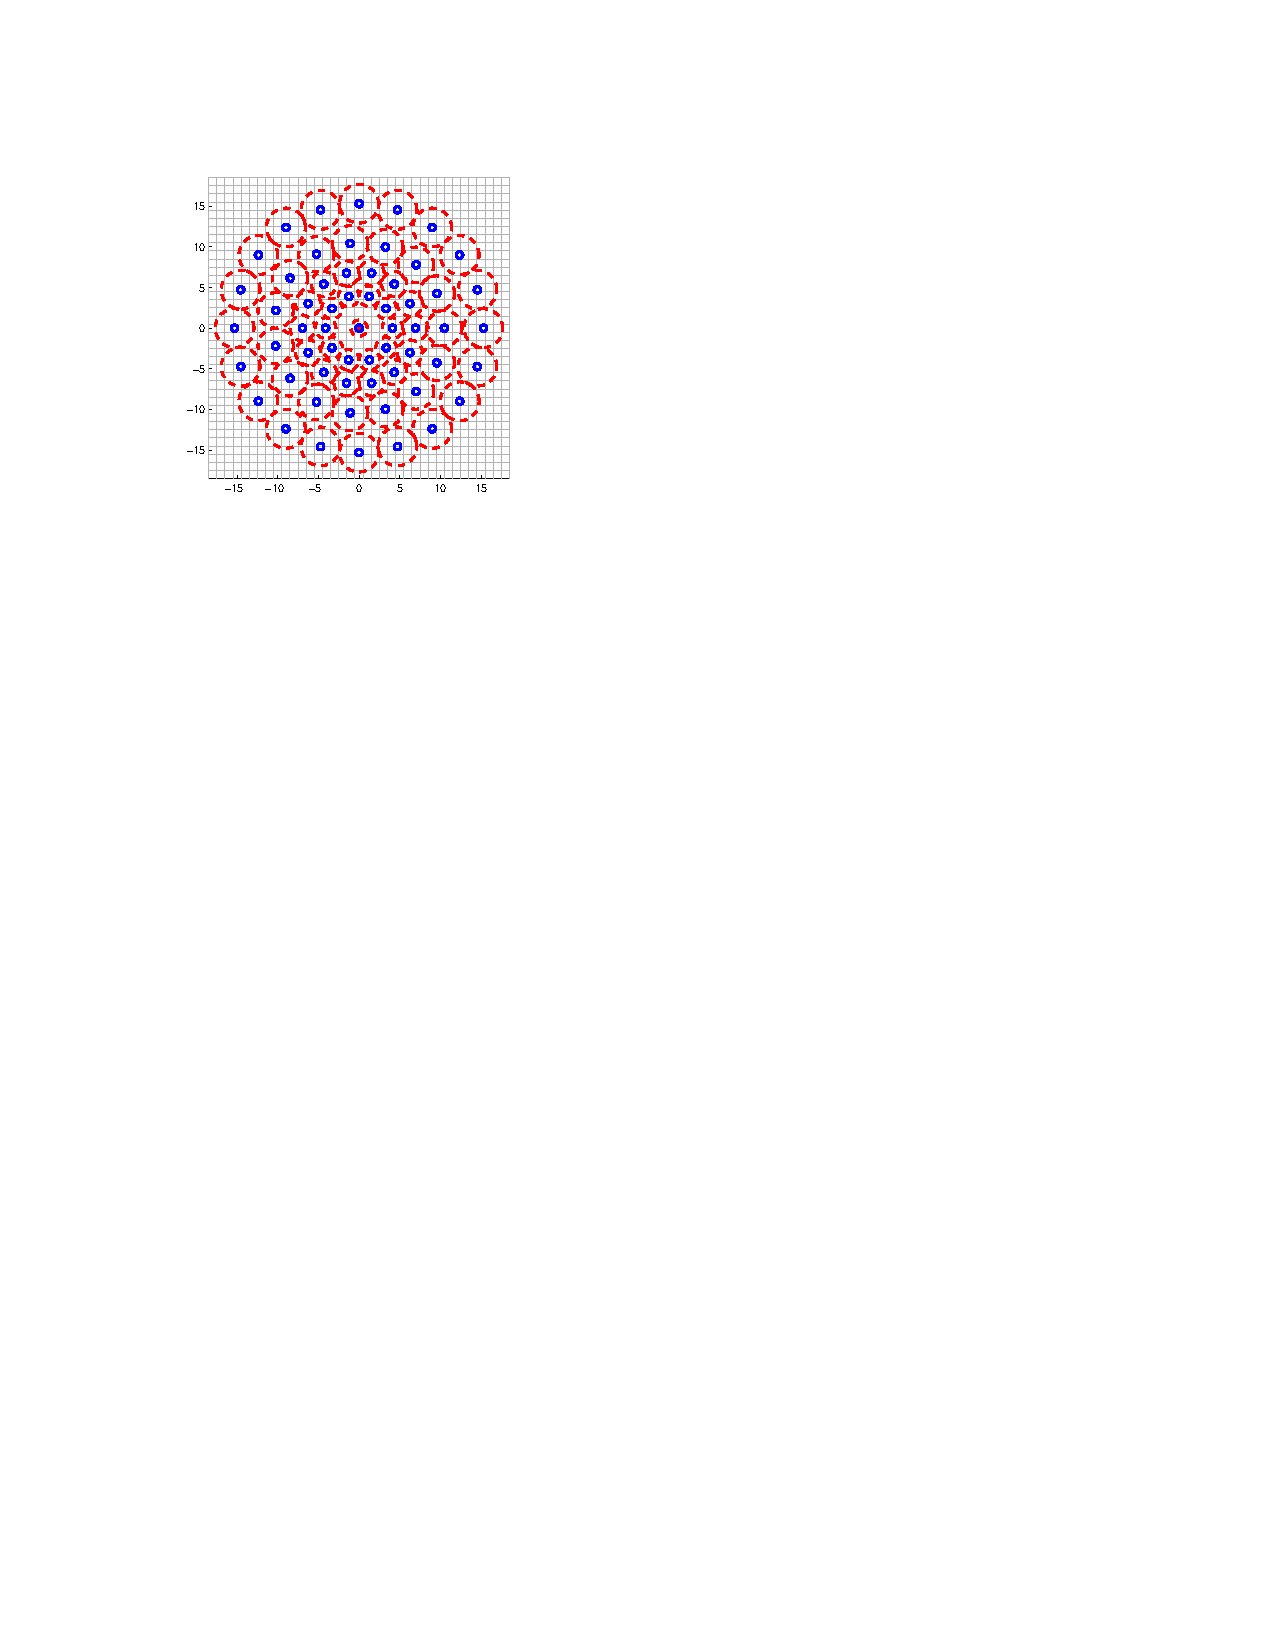
\includegraphics[width=0.8\textwidth]{../Drawings/methods/BRISK_Sampling_Pattern.pdf}
    \caption{The sampling pattern for an interest point. Each blue circle represents a sample and the red circle size is proportional to the amount of smoothing performed on each respective sample}
    \label{fig:samplingPattern}
\end{figure}

The next step is to position and scale the pattern according to the interest points that have been detected. The first step in the procedure is to calculate the gradient between each of the points $(p_i, p_j)$ in the pattern. This gradient is calculated as shown in \eqnref{eqn:gradient}.\\

\begin{equation}
m(p_i, p_j) = (p_j - p_i) \frac{I(p_j, \sigma_j) - I(p_i, \sigma_i)}{||p_j - p_i||^2}
\label{eqn:gradient}
\end{equation}

Following this, the euclidean distance between all possible pairings of the sample points are computed to generate long and short pairs, $L$ and $S$ respectively. The pairings are defined as shown in \eqnref{eqn:pairings}. The thresholds $ \delta_{max},  \delta_{min}$ are chosen as $9.75h$ and $13.67h$ where $h$ is the scale of the interest point $k$. \\   


\begin{eqnarray}
S &=& ((p_i, p_j) \mid ||p_j - p_i|| < \delta_{max})\\
L &=& ((p_i, p_j) \mid ||p_j - p_i|| > \delta_{min})
\label{eqn:pairings}
\end{eqnarray} 

The overall pattern direction for the interest point is determined by computing the overall gradient of all the long pairings $L$ as shown in \eqnref{eqn:longGradients}. Long pairings are used instead of short pairings as it was found that short pairing gradients tend to cancel each other out \citep{Leutenegger2011}. \\

\begin{equation}
\textbf{M} = (m_x, m_y) = \frac{1}{L} \sum_{((p_i, p_j) \epsilon L)} m(p_i,p_j)
\label{eqn:longGradients}
\end{equation}

This gradient is then used to find the angle with which to rotate the sampling pattern around the interest point in order to achive rotation invariance. The angle is computed as shown in \eqnref{eqn:angle}. \\

\begin{equation}
\alpha = atan(\frac{m_y}{m_x})
\label{eqn:angle}
\end{equation}

Once the pattern has been rotated, the descriptor vector is computed. This vector is $512$ bits long and is formed using intensity comparisons between the rotated short distance pairings $S$. Therefore, for each short-distance pairing, a brightness comparison test as shown in \eqnref{eqn:brightness} is performed to yield the descriptor entry $d_k$, $k = 1,2,3...512$.\\

\begin{equation}
d_k = \left\{ \begin{array}{rl}
1 &\mbox{$I(p_j^{\alpha}, \sigma_j) > I(p_i^{\alpha}, \sigma_i)$,} \\
0 &\mbox{Otherwise}
\end{array} \right.
\label{eqn:brightness}
\end{equation}

This produces the rotation and scale invariant descriptor vector.\\
\chapter{Robocup Feature Extraction Techniques}
\label{sec:realtimeFeatureExtraction}
This chapter describes the main feature extraction algorithms that are to be compared in order to determine the best algorithm to be implemented on the Nao humanoid robot. Variations of the original BRISK implementation \citep{Leutenegger2011} have been utilised and include BRISK0, BRISK0 - SURF2D and BRISK0 - U-BRISK. 1D SURF has already been developed and implemented on a Nao robot by the \textit{rUNSWift} Robocup team \citep{Anderson} and is used in this thesis as a means of comparison with the BRISK-based algorithms.\\

In the Robocup scenario, when observing features, the robot's head will be tilted upwards at the maximum possible angle in order to observe features that are on or near the ceiling. This is because in a real Robocup environment, dynamic objects such as humans will be detected as dynamic features. These feature are not necessarily repeatable and will potentially hinder the robot's  ability to match interest points and hence images during the course of the football game.\\

\section{BRISK0 - UBRISK}
\label{sec:brisk0}
In order to make the BRISK algorithm suitable for the Robocup domain, some slight modifications had to be made to the original algorithm. These changes include combining a detector defined as BRISK0, which is a slight variation of the original BRISK implementation, with a variety of descriptors which will be described below. These feature extraction algorithms are applied to a gray-scale image and matching is performed using hamming distance as described in \secref{sec:matching}.\\

\subsection{Image Processing}
\label{sec:imageProcessingBrisk}
Only the upper $300$ pixel rows of the image are utilised for processing.  This should effectively prevent dynamic objects such as humans, found in the lower image portion, from being detected as interest points. In addition to the advantage of generating potentially repeatable features, evaluating only a sub-section of the image results in a significant increase in computational performance. \\ 

The image processing procedure used for the BRISK-based implementations is as follows. Initially a $640 \times 480$ YUV image, captured by the Nao's camera, is converted to a gray scale image as shown in \figref{fig:colourGrayscale}. One of the main reasons for this is that it allows the image to be processed along a single channel which optimises computational performance. \\

\begin{figure}[h!] 
  \centering
    \includegraphics[width=0.8\textwidth]{../Drawings/brisk/yuvImageGray.jpg}
    \caption{Conversion of the YUV image captured by the Nao to grayscale}
    \label{fig:colourGrayscale}
\end{figure}

Since we are only interested in features near the ceiling, the bottom section of the image is cropped and remove before image processing begins. This procedure is shown in \figref{fig:cropImage}.\\

\begin{figure}[h!] 
  \centering
    \includegraphics[width=0.8\textwidth]{../Drawings/brisk/croppedImageFromOriginal.jpg}
    \caption{Cropping the gray scale image for processing}
    \label{fig:cropImage}
\end{figure}

\subsection{Detector}
\label{sec:BRISK0Detect}
The BRISK detector typically detects features by progressively half-sampling an image, and in doing so creates a scale-space pyramid as defined in \secref{sec:brisk}. Creating this pyramid is computationally expensive but generates robust scale-invariant interest points.\\

The scale-space pyramid is not needed for this application since the robot is not expected to undergo significant rotations when re-entering the Robocup field. Thus interest points are only detected along a single scale. This is achieved by setting the number of octaves to zero on the BRISK detector, effectively creating BRISK0. This causes the scale-space pyramid to be `flattened' to a single layer which is utilised to detect interest points. The effect of this is that FAST scores are only computed for a single layer and thus a non-maximal suppression is only performed on this layer in scale space. This results in a significant increase in computational performance. \\

%In addition to this, more features will be detected as the constraint required for detecting an interest point has been relaxed. This is also useful since regions around the ceiling do not usually have a large amount of variation and thus the amount of interest points detected will be relatively limited.\\

A 2D sub-pixel refinement is still applied to the interest points on the single layer, resulting in an increased accuracy in interest point image coordinates.\\

Since only a single octave is utilised and interest points are therefore only detected on a single scale, the 1D parabola that is fitted along the scale-space axis \citep{Leutenegger2011} is also discarded. The disadvantage of this approach is that the local maxima FAST scores are not as accurate as in the original implementation but the increase in accuracy is not crucial in this application as good performance is still obtained as shown in Chapter \ref{sec:experimentsResults}. Furthermore, the increase in computational performance is crucial in developing a method that is practically implementable on the robot. This generates a bank of interest points and the descriptors are then computed.\\

\subsection{Descriptor}
\label{sec:BRISK0Describe}
In order to determine the best feature extraction algorithm to be utilised on the robot, a variety of BRISK and SURF descriptors have been combined with the BRISK0 detector. The descriptors include BRISK0, U-BRISK and 2D SURF descriptors.\\

The BRISK0 descriptor complements the BRISK0 detector and assigns the same scale to all of the interest points. This is because interest points are detected on only a single scale as mentioned previously. The rest of the BRISK algorithm is computed according to the original BRISK implementation resulting in a rotation invariant descriptor of length $512$ bits\citep{Leutenegger2011}.\\

The SURF 2D descriptor is also combined with the BRISK0 detector. This creates a descriptor vector of length $64$ as implemented in 2D SURF \citep{Bay2008}. No modifications have been made to the original 2D SURF descriptor.\\ 

The U-BRISK descriptor contains a slight modification to the original BRISK descriptor. The rotation of the sampling pattern, which was described in \secref{sec:briskDescribe}, has been discarded. This removes the rotation invariant property of the BRISK feature extraction algorithm, but provides a significant increase in computational performance. The brightness comparison tests used to create the descriptor vector are therefore performed on interest points with a sampling pattern that remains in a standard orientation. The combination of BRISK0 and U-BRISK produces the best overall performance for the Robocup scenario as detailed in Chapter \ref{sec:experimentsResults}. \\

\section{1DSURF}
\label{sec:1dsurf}
Another technique that can be utilised for the Robocup is the 1D SURF feature extraction algorithm that has been previously developed and implemented on a Nao robot for Robocup \citep{Anderson}. This algorithm extracts features from a single row of pixels in an image $A$. These features are then matched with features extracted from a row of pixels generated from an image $B$ being compared to image $A$. This technique is a number of orders of magnitude faster than the traditional 2D SURF implementation and is potentially suitable for use in the Robocup \citep{Anderson}.\\

The original implementation of this algorithm has been provided by the \textit{rUNSWift} team and has been utilised as a means of comparison in this thesis \citep{Anderson}. The OpenSURF implementation, which is freely available online \citep{opensurf}, has been utilised by the \textit{rUNSWift} team in order to implement this algorithm.\\

The novelty of this algorithm is transforming 2D SURF into its 1D SURF implementation. This requires changes to both the detector and descriptor and will be explained in the sections to follow.\\

\subsection{Image Processing}
\label{sec:imageProcessing}
The first main step in implementing the 1D SURF algorithm is to extract a single row of gray-scale pixels from the image. This is typically achieved by sampling every fourth pixel intensity value along the robot's horizon line \citep{Bhuman} in order to speed up processing time \citep{Anderson}. A change has been made whereby the pixels are now sampled $120$ pixel rows from the top of the image. This ensures that the algorithm is detecting features near the ceiling and helps prevent dynamic interest points from being detected.\\

In addition to this, each sampled pixel intensity value is summed with a vertical band of $30$ pixels as shown in \figref{fig:rows}. This is performed instead of taking the mean primarily since it is faster to compute. This procedure therefore ultimately generates a row of summed pixel intensities. It is from this row of intensities that features will be extracted and matched.\\

\begin{figure}[h!] 
  \centering
    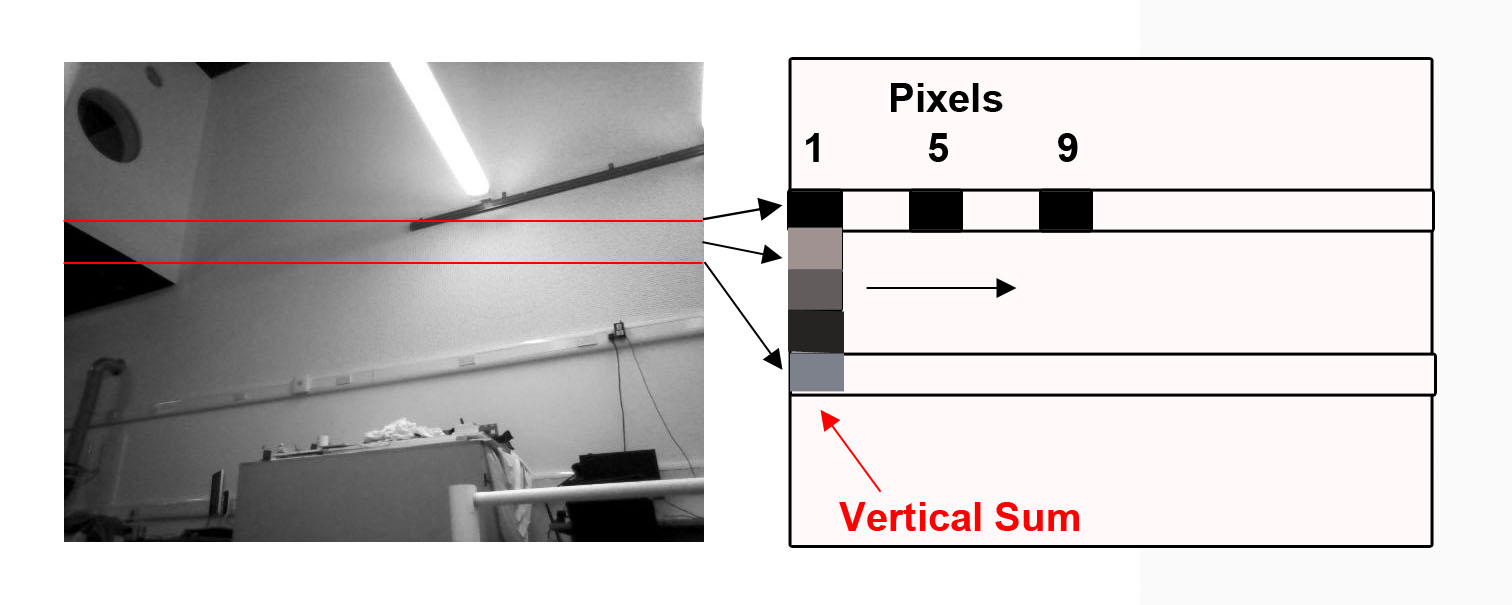
\includegraphics[width=1.0\textwidth]{../Drawings/methods/horizon.jpg}
    \caption{The vertical sum of pixel intensities along a sample horizon line indicated in red. Every fourth pixel is sampled as shown in the right portion of the figure. }
    \label{fig:rows}
\end{figure}

\subsection{Detector}
\label{sec:1dsurfDetect}
The 1D SURF detector has a number of differences from that of its 2D equivalent. The first major difference is the construction of the integral image. The integral image as stated in \secref{sec:integralImages}, allows for fast computation of rectangular areas in an image. Since the image is now 1D, the integral image is only computed along the single row of pixels.\\ 

The next step is calculating the blob response for each point $(x,1)$ along the single row of pixels. In the 2D case this is typically achieved by performing a 2D convolution, convolving a second order Gaussian derivative with the image at the point $\textbf{x} = (x,y)$. The Gaussian is approximated as a box filter and, combined with the integral image, results in a very efficient computation. In the 1D case the convolution can only be computed along the single dimensional row of pixels. Thus, the box filters have been effectively reduced to 1D box filters and the $xy$ and $y$ directional box filters can be neglected. The determinant of the Hessian can thus be reduced to \eqnref{eqn:reducedHessian}.\\

\begin{equation}
det(Hessian) = D_{xx}D_{xx}
\label{eqn:reducedHessian}
\end{equation} 

The number of octaves chosen for 1D SURF is $4$ and the number of scales per octave is $3$. Once a blob response map has been generated, interest points can be subsequently computed for each octave and each scale within the respective octave. Typically, in order to identify local maxima, each pixel in 3D scale space is compared to its $3 \times 3 \times 3$ surrounding neighbors and a non-maximal suppression is performed \citep{Evans2009}. However, in the case of 1D SURF, this constraint is relaxed and the pixel is only compared to its neighbors in the single scale space dimensional as shown in \figref{fig:singleScale} \citep{Anderson}. The result is that more features will be detected. However, these features will not have as strong responses as the features detected in 2D SURF.\\

\begin{figure}[h!] 
  \centering
    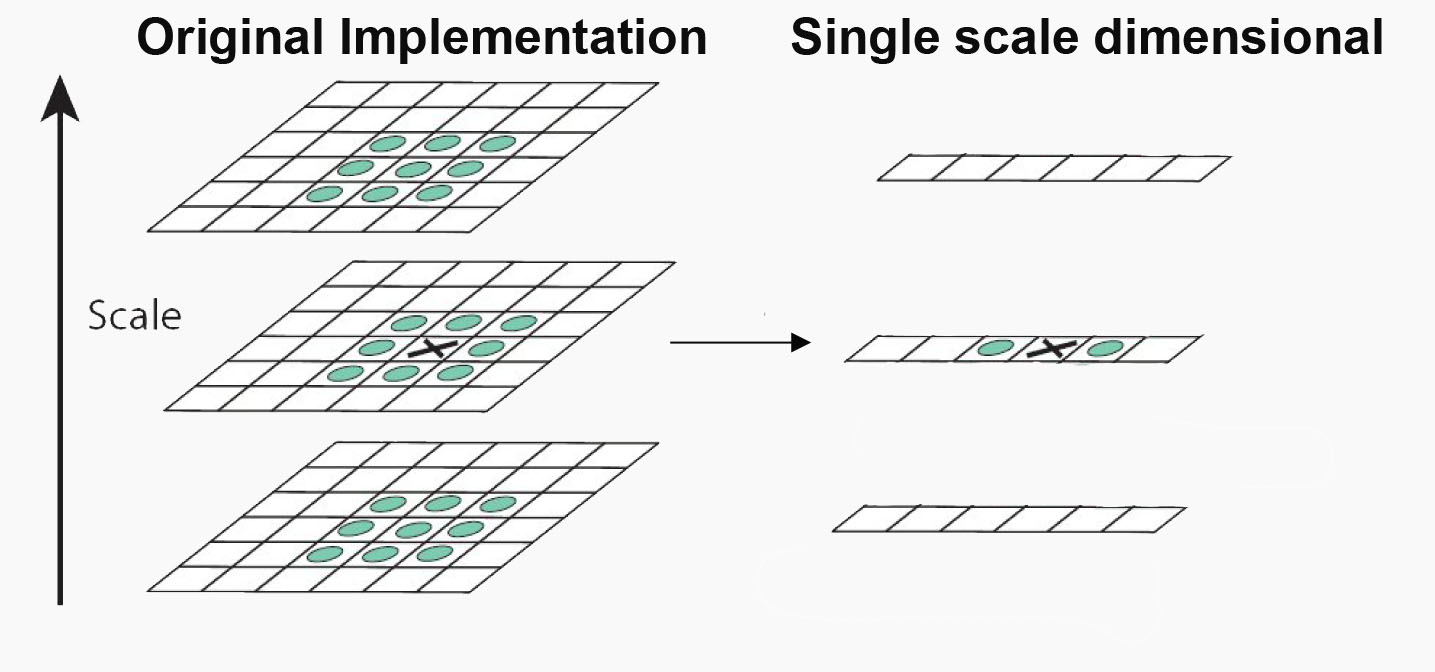
\includegraphics[width=0.8\textwidth]{../Drawings/methods/SURF1D_Nonmaximal_suppression.jpg}
    \caption{1D SURF only uses the single scale dimensional in order to perform non-maximal suppression and detect interest points \citep{Anderson}.}
    \label{fig:singleScale}
\end{figure}

Once this has been achieved, the interest points are usually interpolated in both scale and image space to sub-pixel accuracy \citep{Evans2009}. However, sub-pixel accuracy is not necessary for the Robocup domain and has thus been discarded in the 1D implementation \citep{Anderson}. This procedure ultimately detects a set of interest points along a single row of pixels based on the blob response map. The next step involves computing the descriptors.\\  

\subsection{Descriptor}
\label{sec:1dsurfDescribe}
Typically, the 2D SURF descriptor is constructed in two stages. The first stage involves assigning an orientation to the descriptor and has been described in \secref{sec:2dsurfdescribe}. This step has been discarded since the feature points are assigned with reference to the horizon line and therefore do not require an orientation.\\

In 2D SURF, the second stage involves constructing a square region around the interest point and sub-dividing the region into $16$ equally-sized sub-regions as detailed in \secref{sec:2dsurfdescribe}. For each sub-region HWRs in both the $x$ and $y$ directions are calculated for $25$ regularly spaced sample points. These responses are summed together to produce $4$ descriptor values for the sub-region corresponding to \eqnref{eqn:descriptorSub}. Therefore, in total a descriptor vector of length $64$ is created.\\

In the case of 1D SURF, it is only possible to utilise $4$ of the $16$ sub-regions along the $x$ direction as shown in \figref{fig:subregions4} due to the reduction in dimensionality of the image. In addition, HWRs can only be calculated along the $x$ direction which allows for the $y$ direction Haar Wavelets to be discarded. The current implementation of 1D SURF further reduces the number of sub-regions to $3$ while still achieving good performance \citep{Anderson}. This will ultimately produce a $6$ dimensional descriptor vector rather than the $64$ dimensional descriptor vector as shown in \eqnref{eqn:descriptor1d}. Each of the $3$ sub-regions will produce a descriptor pair of $[\sum dx_i, \sum |dx_i|]$ where $dx_i$ refers to the HWR from the $i^{th}$ sub-region in the $x$ direction. \\

\begin{figure}[h!] 
  \centering
    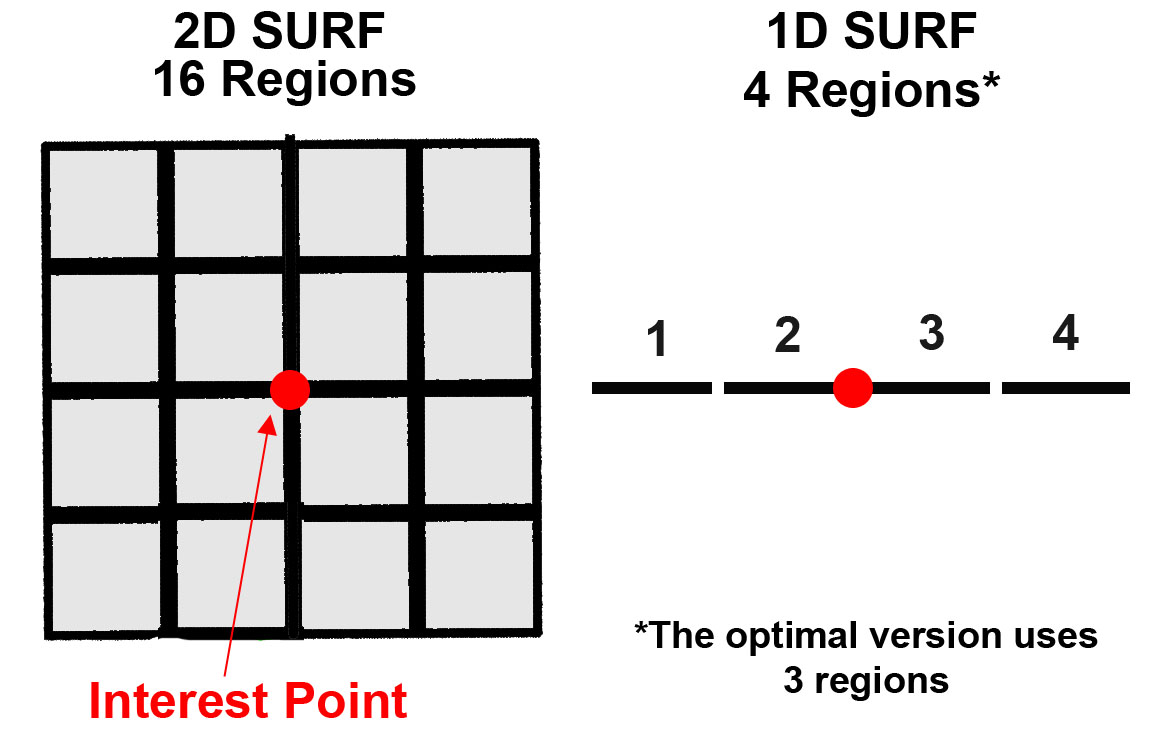
\includegraphics[width=0.5\textwidth]{../Drawings/methods/SURF1D_Descriptor.jpg}
    \caption{Using only 4 sub-regions (3 in the optimal case) to compute the descriptors for each interest point}
    \label{fig:subregions4}
\end{figure}


\begin{equation}
descriptor = [ \sum dx_1, \sum |dx_1|,\sum dx_2, \sum |dx_2|,\sum dx_3, \sum |dx_3|] 
\label{eqn:descriptor1d}
\end{equation}
\chapter{Feature Matching}
\label{sec:matching}
Once the interest points have been detected and the descriptors have been computed, the interest points can be matched between pairs of images. This is achieved by first calculating the distance in feature space between the interest point descriptors in each image. The interest points are then matched if their descriptor distances are within various thresholds or constraints of one another as pre-defined by the matching technique that is being utilised. An example of matches found from comparing a pair of images is shown in \figref{fig:matchesIntro}. Matched interest points in corresponding images are connected by a green line as seen in the figure. Interest points that have not been matched are represented by red circles.\\

\begin{figure}[h!] 
  \centering
    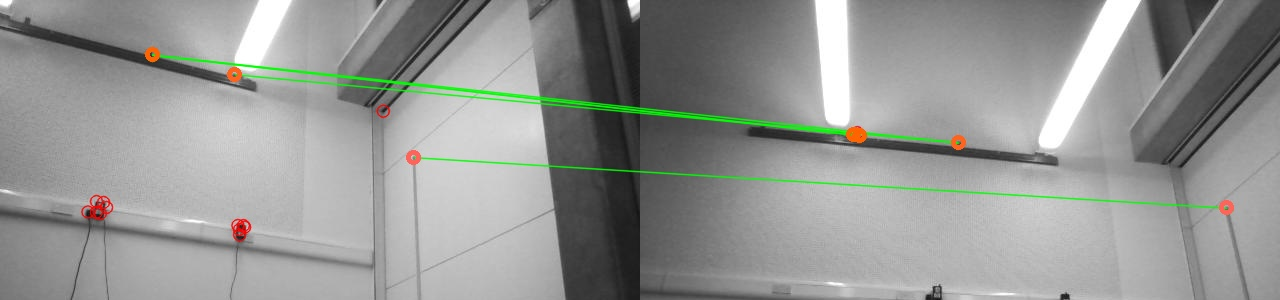
\includegraphics[width=0.8\textwidth]{../Drawings/Matching/MainRobocupDataset.jpg}
    \caption{An example of matches between a pair of images. The matches are connected by green lines.}
    \label{fig:matchesIntro}
\end{figure}

The methods used to calculate the distance between interest point descriptors will be detailed. The various constraints imposed to determine whether a match between two interest points is indeed valid will be described in \secref{sec:validation}. In addition to this, the various matching techniques utilised to match interest points will be detailed in \secref{sec:matchingTechniques}.\\

\section{Calculating Distance between Feature Descriptors}
\label{sec:distance}

\subsection{Hamming Distance}
\label{sec:hamming}
The Hamming distance is a measure of the distance between two strings \citep{Banzal2007}. The distance between two strings is defined as the number of corresponding bits, letters or numbers that differ between these strings. Assume two strings, $A$ and $B$, of equal length. In this example, these strings can only take values of $0$ or $1$. The Hamming distance is then calculated by determining whether or not the values of corresponding elements in each of the strings are different. If the values are different, then the Hamming distance is incremented by a value of $1$.\\

This metric is used to determine the distance between interest point descriptors in the BRISK algorithm \citep{Leutenegger2011}. Since the interest point descriptors, as mentioned in \secref{sec:briskDescribe}, are vectors of $512$ bits in length, the Hamming distance of two descriptors is calculated by determining how different the first descriptor is from the second in feature space. The bits can only take values of $0$ or $1$. It is desired that the descriptors are as similar as possible for the descriptors to be a match; that is, they have a low Hamming distance value. \\

This is a very efficient algorithm and has been effectively performed in BRIEF \citep{Calonder}. It consists of $512$ XOR operations between corresponding bits followed by a bit count. This is a very efficient computation to perform on modern day architectures \citep{Leutenegger2011}. \\ 

\subsection{Euclidean Distance}
\label{sec:euclidean}
In SURF-based approaches,  the Euclidean distance is used as a metric to determine whether or not there is a match between two interest point descriptors \citep{Lowe2004}. Given two interest point descriptors of length $64$, the Euclidean distance is calculated between descriptors in feature space and results in a value indicating the difference between the two descriptors. As in BRISK, it is desired that the Euclidean distance is as small as possible between the descriptors for them to be a match. A match occurs if the nearest neighboring feature descriptor corresponding to an interest point in image $A$ is within a predefined Euclidean distance from the descriptor of the corresponding matched interest point in image $B$.\\

In addition to this, in order to speed up matching, the sign of the Laplacian which is the trace of the Hessian matrix, is used to determine whether or not each \textit{blob response} in the respective images are of a similar contrast \citep{Bay2008}. The sign of the Laplacian determines whether the interest point in question is a dark blob on a light background or a light blob on a dark background. This enables interest points of different contrasts to be rejected as matches without having to compute the Euclidean distance between the descriptors.\\

\section{Validating Matched Features}
\label{sec:validation}
Once the Hamming or Euclidean distance is computed between two descriptors and the resulting distance is within a predefined threshold, the corresponding interest points are considered to be a match. However, this match may not necessarily be a valid match and a number of constraints have been imposed in order to verify the match.\\

\subsection{2-Nearest Neighbors Ratio}
\label{sec:2nnMatching}
The 2-NN Ratio is computed using the closest and second closest match for a particular interest point as shown in \eqnref{eqn:2nnRatio} \citep{Lowe2004}. This constraint therefore requires that each interest point has at least two matches. This is performed for every detected interest point in the image being evaluated. It has been assumed that each interest point has only a single, unique corresponding match between a pair of images. Based on this assumption, the closest match should be the true matching interest point in the corresponding image, whereas the second closest match should belong to a different object in the image and hence is an invalid match.\\

\begin{equation}
Ratio_{2-NN} = \frac{\mbox{Closest Match}}{\mbox{Second Closest Match}}
\label{eqn:2nnRatio}
\end{equation}

Therefore, for a valid match between interest points, the closest match should be significantly closer than the second closest match (which is the closest incorrect match) from the interest point that is being evaluated \citep{Lowe2004}. This means that a valid interest point match should generally have a lower 2-NN ratio than an invalid match. An invalid match will probably have a number of matches within a similar distance of one another due to the high dimensionality of the feature space \citep{Lowe2004}. The feature space as mentioned previously is of dimensionality $64$ for 2D SURF and $512$ for BRISK-based techniques.\\

Based on the results in \secref{sec:knnMatchingConstraint}, all interest point matches with a 2-NN ratio above $0.7$ are rejected as invalid matches whereas all matches with a threshold below this value are accepted as valid matches. An example of the 2-NN constraint can be seen in \figref{fig:2nn_1} and \figref{fig:2nn_2}. \figref{fig:2nn_1} shows the interest points in the left image where each interest point has two matches in the right image. After applying the 2-NN ration constraint, a number of invalid matches are discarded and the best match for each interest point is displayed  as seen in \figref{fig:2nn_2}.\\


\begin{figure}[h!] 
  \centering
    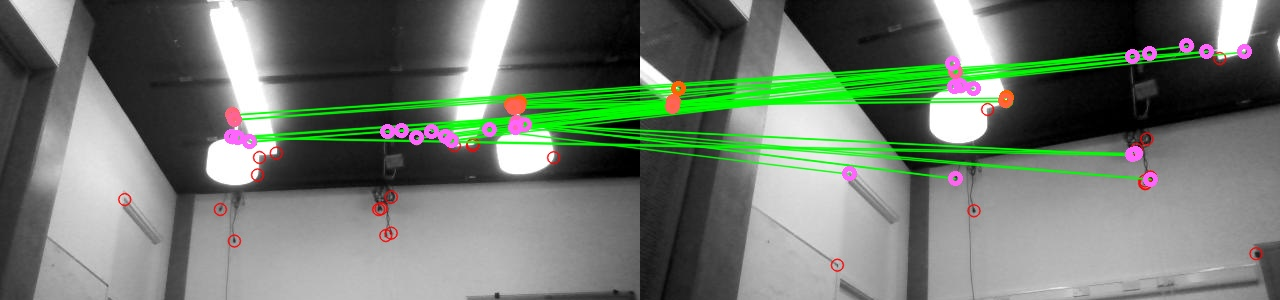
\includegraphics[width=0.8\textwidth]{../Drawings/Matching/feature_matching/dataset_2nn_matching_constraint_before.jpg}
    \caption{Matched interest points before applying the 2-NN ratio constraint}
    \label{fig:2nn_1}
\end{figure}

\begin{figure}[h!] 
  \centering
    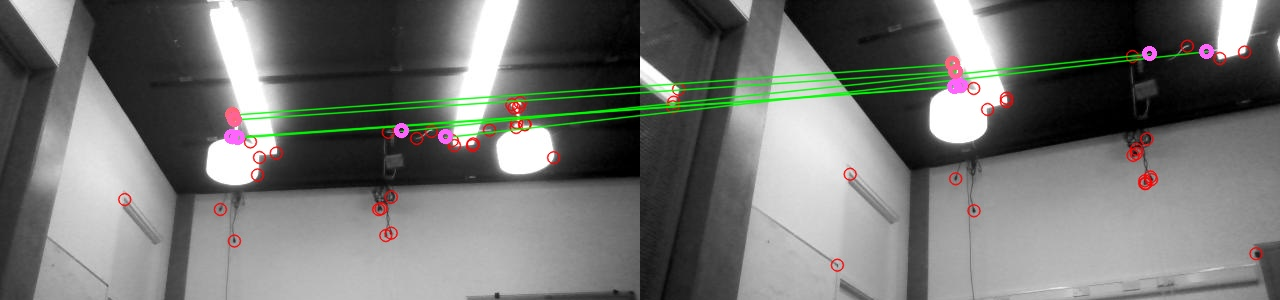
\includegraphics[width=0.8\textwidth]{../Drawings/Matching/feature_matching/dataset_2nn_matching_constraint_after.jpg}
    \caption{The best matches are displayed after having applied the 2-NN ratio constraint}
    \label{fig:2nn_2}
\end{figure}


\subsection{Angle and Distance Constraints}
\label{sec:angleDistanceConstraints}
Two novel matching constraints have been developed during this thesis in order to determine whether or not a match between two interest points in corresponding images are valid; namely, the angle and distance constraints respectively. A pair of interest points have to fulfil both of these constraints in order to be considered a valid match. In order to verify that the match fulfils these constraints, the pair of images that are being evaluated are placed next to one another as shown in \figref{fig:angleConstraint}. A line is then connected between each pair of matched interest points as shown in \figref{fig:angleConstraint} and \figref{fig:distanceConstraint}. It is this line that is used to determine whether the matched pair of interest points are valid.\\

The angle constraint calculates the angle from the interest point in the left image relative to the interest point in the right image. It has been determined through visual analysis that the angle between two matched interest points should be less than  $10^{\circ}$. This is because corresponding matches should be placed at approximately the same height provided there are no large image rotations. Since Robocup is the immediate application, negligible rotation is expected while the robot is localising itself. If the angle is within the pre-defined threshold then the match is valid, otherwise it is invalid. As can be seen in the figure, $\alpha$ is larger than the pre-defined threshold and therefore the match is marked as invalid. $\beta$ is within the threshold and therefore pertains to a valid match. \\

The distance constraint states that the length of the line connecting two matched interest points should be the width of the image plus a pre-defined threshold. This constraint assumes no significant scale changes which is again feasible based on the current application domain. A pre-defined threshold of $200$ pixels has been chosen based on visual analysis. As can be seen in \figref{fig:distanceConstraint}, the longer line does not pass the distance constraint and is marked as being invalid.\\

\begin{figure}[ht!]
\begin{minipage}[b]{0.5\linewidth}
  \centering
    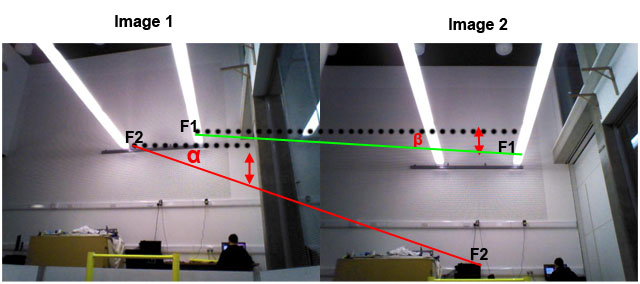
\includegraphics[width=1.0\textwidth]{../Drawings/constraints/angleConstraintMerged.jpg}
    \caption{The angle constraint that has been developed to remove invalid matches} 
    \label{fig:angleConstraint}
\end{minipage}
\begin{minipage}[b]{0.5\linewidth}
  \centering
    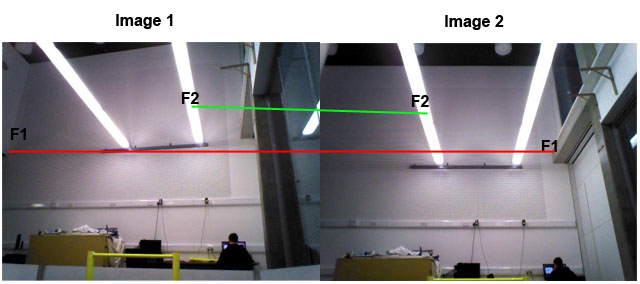
\includegraphics[width=1.0\textwidth]{../Drawings/constraints/distanceConstraint.jpg}
    \caption{The distance constraint that has been developed to remove invalid matches} 
    \label{fig:distanceConstraint}
\end{minipage}
\end{figure}

%\begin{figure}[h!] 
%  \centering
%    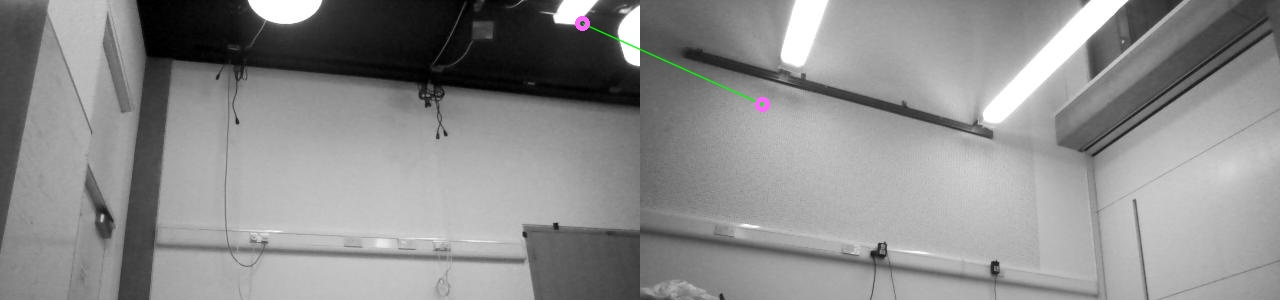
\includegraphics[width=0.8\textwidth]{../Drawings/constraints/t_20_hd_55_OG_Left_MG_Right_2_12.jpg}
%    \caption{An incorrect match detected due to an angle larger than $10^\circ$}
%    \label{fig:imagesSide}
%\end{figure}


\section{Interest Point Matching Techniques}
\label{sec:matchingTechniques}
Three main interest point matching techniques have been utilised in this thesis. Both BRISK and 2D SURF-based approaches make use of 2-Nearest Neighbors and Radius Matching. A matching technique called Nearest Neighbors with RANSAC has been developed by the \textit{rUNSWift} Robocup team \citep{Anderson}. This technique will be referred to as RANSAC matching and is used for the 1D SURF feature extraction algorithm. These interest point matching techniques assume that interest points with corresponding descriptors in image $A$ (query image) are being compared to interest points with their corresponding descriptors in image $B$ (stored image). \\

\subsection{2-Nearest Neighbours Matching}
\label{sec:knn}
The 2-Nearest Neighbors (2-NN) interest point matching technique involves finding two interest points in image $B$ that yield the closest matches to the interest point that is currently being evaluated in image $A$. This technique ensures that two matches will be found for every interest point in the query image $A$. Therefore the number of matches is always twice the total number of interest points in the query image.\\

The algorithm is implemented as follows. Initially, the interest points in both the stored and query images are detected. Their descriptors are computed and all of the descriptors in the query and stored image pair are sent into the 2-NN matching algorithm. The Hamming/Euclidean distance in feature space (depending on the method) between each query descriptor and all of the stored descriptors is then calculated. The top two stored descriptors yielding the lowest Hamming/Euclidean distances are assigned as matches to the query descriptor. These matches are stored in descending order where the first match has the lower of the two distances. An example of three interest points, in query image $A$, with two corresponding matches each in the stored image $B$, is shown in \figref{fig:2nn_matching}. \figref{fig:2nn_best_match} shows the best match for each of the interest points.\\

It must be noted that both the 2-NN ratio constraint and the angle and distance constraints respectively are applied to this matching technique.\\

 \begin{figure}[h!] 
  \centering
    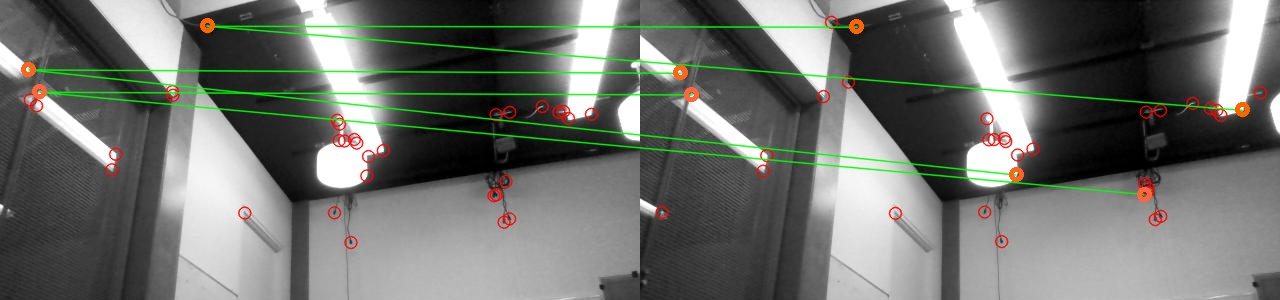
\includegraphics[width=0.8\textwidth]{../Drawings/Matching/feature_matching/dataset1_without_validation_knn.jpg}
    \caption{The interest points in the left image (image $A$) and their corresponding 2-NN matches in the right image (image $B$)}
    \label{fig:2nn_matching}
\end{figure}

 \begin{figure}[h!] 
  \centering
    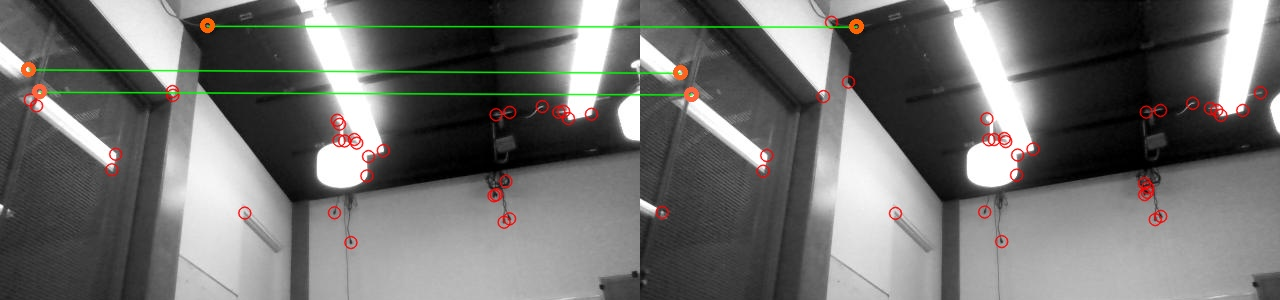
\includegraphics[width=0.8\textwidth]{../Drawings/Matching/feature_matching/dataset1_without_validation_knn_best.jpg}
    \caption{The best matched interest points}
    \label{fig:2nn_best_match}
\end{figure}

\subsection{Radius Matching}
\label{sec:radius}
Radius matching is different from 2-NN in that a match between a pair of interest points only occurs if the calculated Hamming or Euclidean distance (depending on the feature extraction algorithm being used) is below a pre-defined threshold. This threshold is denoted the `Hamming distance' for BRISK-based algorithms and the `Euclidean distance' for 2D SURF-based algorithms. \\

This method does not guarantee that every interest point in the query image will have a corresponding match in the stored image. In contrast, this method does not limit the amount of matches for an interest point in the query image.\\

The Radius Matching algorithm therefore computes the descriptors for all of the interest points in both the query and stored images respectively. The descriptors are then matched if the distance in feature space is below the pre-defined threshold. These matches are sorted and stored in ascending order where the first match has the smallest Hamming/Euclidean distance. Matches generated from Radius Matching can be seen in \figref{fig:radius_match}. Here, one of the interest points in the query image (left image) has more than two matches with interest points in the stored image (right image). The best matches for this pair of images is shown in \figref{fig:radius_best_match}.\\ 


 \begin{figure}[h!] 
  \centering
    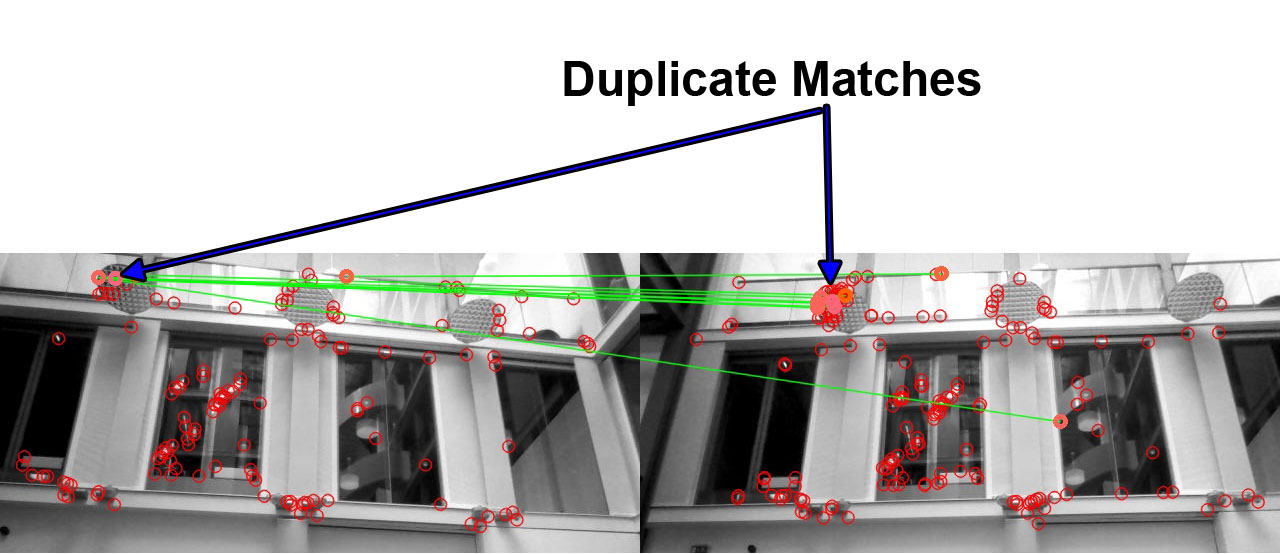
\includegraphics[width=0.8\textwidth]{../Drawings/Matching/feature_matching/dataset1_without_validation_radius_photo.jpg}
    \caption{Matched interest points due to Radius Matching. Note the interest point with more than two matches.}
    \label{fig:radius_match}
\end{figure}

 \begin{figure}[h!] 
  \centering
    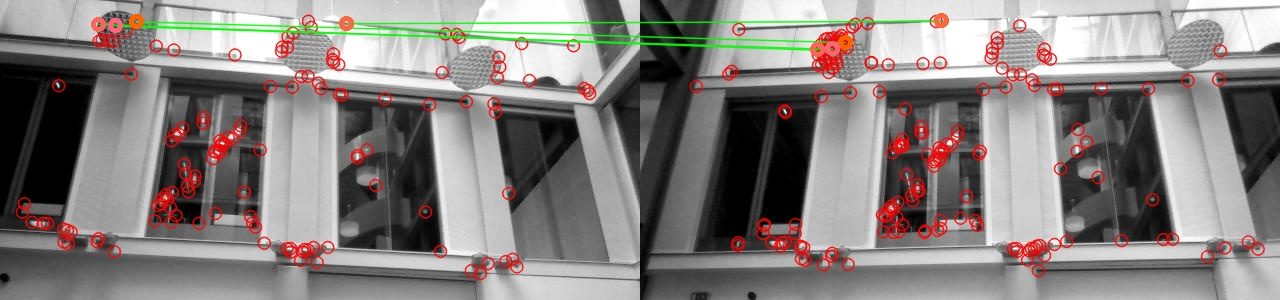
\includegraphics[width=0.8\textwidth]{../Drawings/Matching/feature_matching/dataset1_without_validation_radius_best.jpg}
    \caption{The best matched interest points using Radius Matching}
    \label{fig:radius_best_match}
\end{figure}

\subsection{RANSAC Matching}
\label{sec:ransacMatching}
The RANSAC matching technique has been developed for the 1D SURF implementation \citep{Anderson}. This technique is composed of two stages, namely Nearest Neighbors followed by RANSAC. The nearest neighbors stage calculates the distance in feature space from the first and second nearest neighbor to the interest point being evaluated. It then calculates the 2-NN ratio defined in \secref{sec:2nnMatching} to determine whether the match is indeed valid. The pre-defined threshold for this implementation is $0.75$.\\

Once this stage has been processed, the RANSAC procedure is initialised. This stage removes interest points that do not conform to a straight line function defined in \eqnref{eqn:straightLine} \citep{Anderson}. Here, $x_{query,i}$ is the x position of the $i^{th}$ matched interest point along a single row of pixels in the query image $A$.  $x_{stored,i}$ is the interest point's x position in the stored image $B$. $\beta_s$ and $\beta_d$ are scaling and displacement parameters.\\

\begin{equation}
x_{query,i} = \beta_s x_{stored,i} + \beta_d
\label{eqn:straightLine}
\end{equation} 

To illustrate the meaning of this function, consider \figref{fig:ransacOverview}. The query image $A$ is the bottom image and the stored image is the top left image. Note that the stored image has been rotated clockwise by $90^{\circ}$ for visualisation purposes. The single row of pixels used to detect features can be seen at the top of each image. The single row of pixels have been computed using the pixels within the two red bands in each image as described in \secref{sec:1dsurf}. The $i^{th}$ match generated from the 2-NN ratio is shown in \figref{fig:ransacExample}. The x position for each image is computed and placed into \eqnref{eqn:straightLine}. If $x_{query,i} - (\beta_s x_{stored,i} + \beta_d) \leq P$ where $P$ is a pre-defined threshold, then the interest points are a valid match. If the interest points are valid, then the inverse distance in feature space between the pair of interest points' feature descriptors is computed and is added to a scoring function. Invalid interest points are discarded. This procedure removes outliers and provides a score of how well a pair of images match one another \citep{Anderson}.\\


\begin{figure}[ht!]
\begin{minipage}[b]{0.5\linewidth}
  \centering
    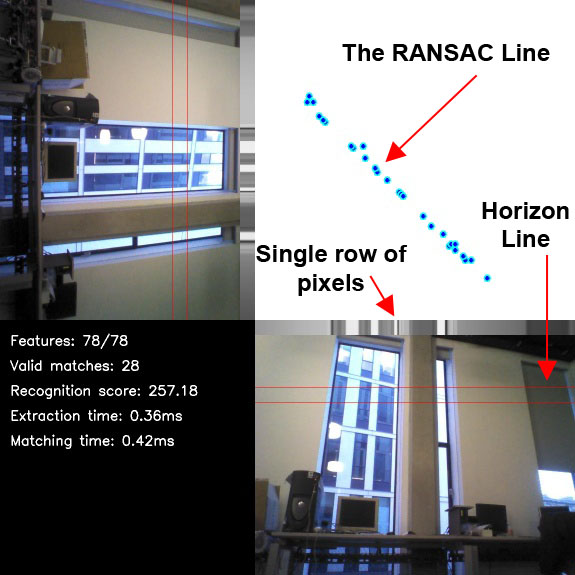
\includegraphics[width=0.8\textwidth]{../Drawings/constraints/matchingLabelled.jpg}
    \caption{An overview of the matching constraints imposed in the 1D SURF algorithm} 
    \label{fig:ransacOverview}
\end{minipage}
\begin{minipage}[b]{0.5\linewidth}
  \centering
    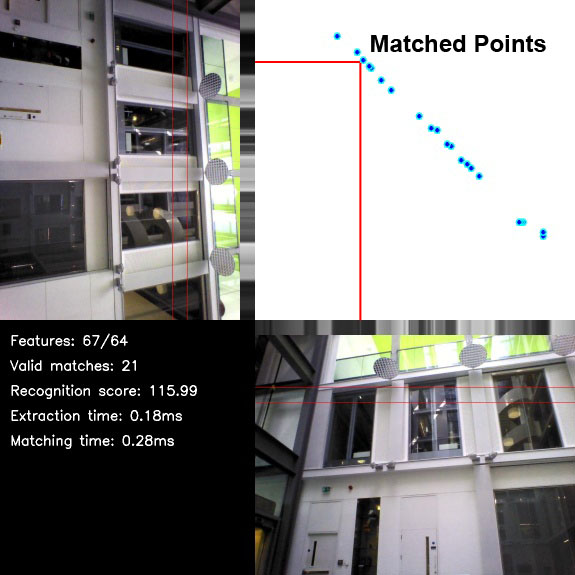
\includegraphics[width=0.8\textwidth]{../Drawings/constraints/matchedPoints.jpg}
    \caption{An example of how the matches are constructed} 
    \label{fig:ransacExample}
\end{minipage}
\end{figure}
\chapter{Localisation}
\label{sec:localisation}
The Nao robot used for this thesis utilises the codebase developed by the \textit{Bhuman} Robocup team \citep{Bhuman}. This codebase has been extended by the \textit{Edinferno} Robocup team based in Edinburgh \citep{edinferno}. A modification to the current Robocup localisation algorithm is proposed in this Chapter to incorporate visual landmarks (\textit{interest points}).\\

This modification to the localisation algorithm is currently applicable when the robot is re-entering the football field after having served a ban for committing a \textit{Standard Removal Penalty}\citep{Rules}. This penalty is initiated if the robot commits a foul on an opposition robot. In this scenario, the robot is removed from the field for $30$ seconds, facing away from the field of play. Once the ban ends, the robot is placed on the halfway line or the nearest possible position along the line.  \\

The robot then has to localise itself after which it can continue to participate in the game. The Nao robot is able to perform localisation as it is initially given a map of the Robocup football field. It typically uses observations such as the goalposts, line segments and corners as inputs to the current localisation algorithm in order to localise itself on the field \citep{Bhuman}. However, since the goalposts are now the same colour, the robot will be unsure as to which side of the field it is on, introducing ambiguities regarding its position.\\

Therefore, this chapter proposes a modification to the current localisation algorithm. The algorithm will incorporate visual landmarks detected by a feature extraction algorithm as new observations. The robot will detect various persistent visual landmarks in the environment. Once the robot recognises these visual landmarks, it uses them in the modified localisation algorithm in order to disambiguate its position on the field.\\

The current localisation algorithm implemented in the codebase is the \textit{Augmented} Monte Carlo Particle Filter (AMCPF)\citep{Laue}. A proposed modification to this algorithm has been made to incorporate the visual landmarks.\\

\section{Augmented Monte Carlo Particle Filter}
\label{sec:amcpf}
The Augmented Monte Carlo Particle Filter (AMCPF) represents the belief or probability of the robot being in a certain position $x$ at time $t$ by $bel(x_t)$ \citep{Thrun2002}. This is a variation of Monte Carlo Particle Filter (MCPF) \citep{Thrun2002} and has the advantage of enabling the robot to overcome the \textit{kidnapping} problem \citep{Thrun2002}, which occurs when the robot faces a \textit{Standard Removal Penalty}. \\

The AMCPF algorithm is presented in \figref{fig:augmented} \citep{Thrun2002}. The variable $x_t^{[m]}$ represents the $m^{th}$ hypothesis (often referred to as \textit{particle}) that the robot is at position $(x,y)$ at time $t$. The variable $w_t$ represents the importance weight which gives an indication of the likelihood of the previous hypothesis being correct. $\bar{\chi}_t$ stores the set of $m$ particles $x_t^{[m]}$ and their corresponding important weights $w_t^{[m]}$ as a two-tuple. $u_t$ represents the control input a time $t$ and $z_t$ represents the observation at time $t$. \\

The algorithm works as follows. Initially the previous set of particles $\chi_{t-1}$ as well as the current control input $u_t$, the current observation $z_t$ and the number of particles $m$ are input into the algorithm. Each particle from the previous set is then fed into the \textit{motion model}, in line $5$ which adds the control input and some additional noise to each particle. This generates the current particle $x_t$. $x_t$ is then given an importance weight by inputting it into the \textit{Measurement Model}. This uses the observation $z_t$ to determine how likely the hypothesis $x_t$ is compared to the actual measurement. A weight $w_t^{[m]}$ is then assigned to the $m^{th}$ hypothesis. The two-tuple is then added to the current particle set $\bar{\chi}_t$.\\

It is at this point that the AMCPF diverges somewhat from the MCPF. The empirical measurement likelihood $w_{avg}$ is computed in line $8$ \citep{Thrun2002}. This is computed in order to determine whether or not random particles should be injected into the algorithm. This is crucial when dealing with the \textit{kidnapping problem} that the robot faces after serving its \textit{Standard Removal Penalty}. If the robot re-enters the field and all particles have been assigned weights of zero, then no particle will be redrawn and the robot will not be able to recover its position. Short and long term averages, $w_{slow}$ and $w_{fast}$, of this likelihood are maintained with their respective decay rates $\alpha_{slow}$ and $\alpha_{fast}$ in lines $10$ and $11$. It should be noted that $0 \leq \alpha_{slow} \ll \alpha_{fast}$. The main point of this algorithm is in line $13$ where particles are redrawn with probability equal to $max(0, 1.0 - \frac{w_{fast}}{w_{slow}})$. This ensures that if the short term decay rate diverges suddenly, then random particles will be injected into the algorithm ensuring that the robot can recover its position if it gets lost.\\

Particles are then redrawn with probability proportional to their importance weights in line $16$ replacing the particles in the particle set $\chi_t$.  

\begin{figure}[ht!]
\begin{minipage}[b]{0.5\linewidth}
  \centering
    \includegraphics[width=1.2\textwidth]{../Drawings/localisation/MCLAugmentedOriginal.pdf}
    \caption{The Augmented Monte Carlo particle Filter Algorithm}
    \label{fig:augmented}
\end{minipage}
\begin{minipage}[b]{0.5\linewidth}
  \centering
    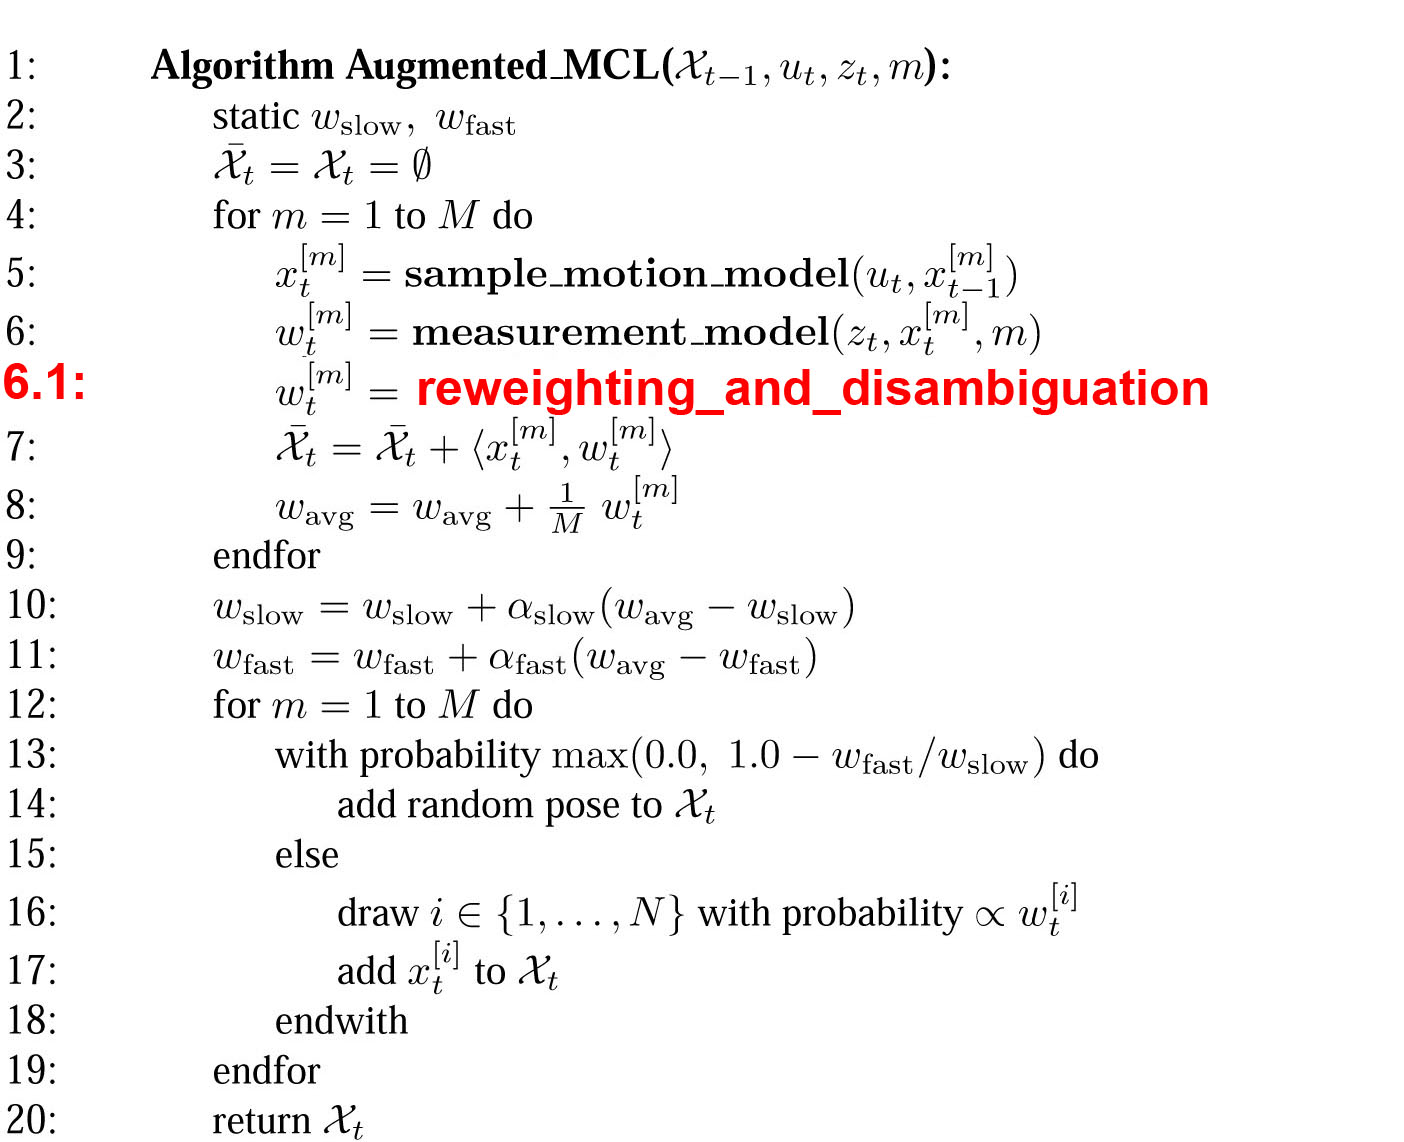
\includegraphics[width=1.2\textwidth]{../Drawings/localisation/MCLAugmented.jpg}
    \caption{The proposed implementation of the method in the Monte Carlo Algorithm \citep{Thrun2002}}
    \label{fig:mclProposed}
\end{minipage}
\end{figure}


\section{Proposed Modification}
\label{sec:modification}
The proposed modification is to add an extra re-weighting routine to the AMCPF algorithm as shown in \figref{fig:mclProposed}. This routine entitled \textit{Reweighting and Disambiguation} will only be called when the robot re-enters the football field after serving a penalty ban. The observations $z_t$ for this routine will be the interest point descriptors computed using the feature extraction algorithm. Once the robot has been able to disambiguate its position, then the AMCPF algorithm will return to its normal operation as shown in \figref{fig:augmented}.\\

\section{Localisation using Natural Visual Landmarks}
\label{sec:localisationNaturalVisualLandmarks}
The localisation algorithm is broken down into a number of sub-routines. These include the initialisation routine, the re-localisation procedure on re-entering the field, the descriptor matching and finally disambiguation.\\

\section{Initialisation Routine}
\label{sec:initialisation}
The first step in localising the robot occurs prior to the start of the game. The robot will initially capture a set of $m$ images of regions behind each of the goal posts. The interest points will be detected using the feature extraction algorithm for each image, and descriptors for these interest points will be computed and stored by the robot for the remainder of the game. These descriptors represent the visual landmarks and the set of computed descriptors will be referred to as $d_{initial}^i |i = 1,2...m$ where $i$ represents the image number. It is assumed that these visual landmarks are persistent throughout the game. However, this is the initial proposal and the features can be updated during the course of the game as a future addition.\\

\section{Re-localisation Procedure}
\label{sec:relocalisation}
When a penalty occurs and a robot is removed from the field, it has to relocalise itself on re-entering the field after it has served the penalty ban. As mentioned previously, the robot is placed on the half-way line or the nearest spot from the half-way line once the penalty period has ended. The example figures below portray the scenario that occurs when the robot re-enters the field from the half-way line on the left-hand side of the field. This will be the example scenario used to describe the algorithm.\\

The robot always enters play on its team's side of the field. However, ambiguities arise as it does not know which position on its side of the field it currently occupies as well as its current orientation. At this point, the robot receives a list of visual landmarks that are present on the football field. These include the goal posts, line segments, line crossings (intersections between line segments) and the center circle \citep{Bhuman}. These are illustrated in \figref{fig:localiseLandmarks}. Using these visual landmarks, the AMCPF algorithm re-weights the particles and the robot knows that it is in one of two locations due to the symmetrical nature of the football field. The possible locations are illustrated in \figref{fig:before} and \figref{fig:beforeSim}. \figref{fig:beforeSim} is a screenshot from the \textit{BHuman SimRobot Simulator} \citep{Bhuman}. As can be seen in the figures, each potential location is represented by a dense cluster of particles. In addition, random particles will also be present due to the particle injection property of the algorithm.\\

\begin{figure}[ht!]
  \centering
    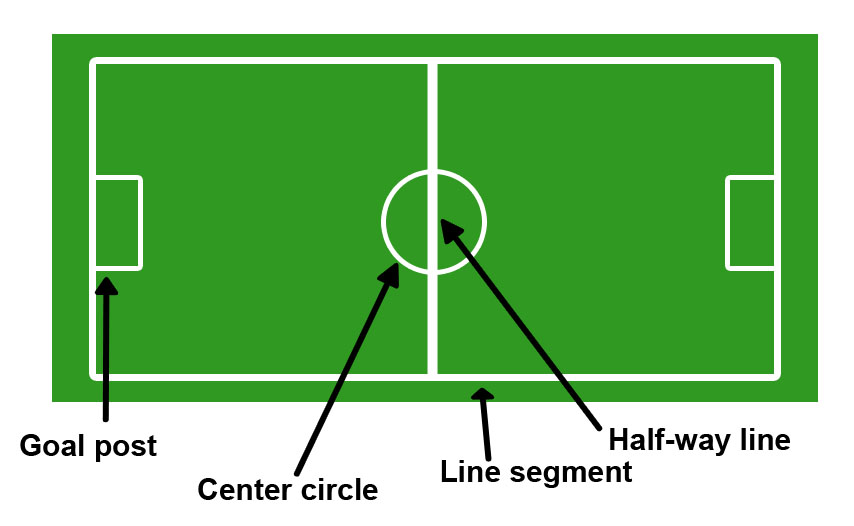
\includegraphics[width=0.4\textwidth]{../Drawings/localisation/goalSetup.jpg}
    \caption{The visual landmarks available on the football field} 
    \label{fig:localiseLandmarks}
\end{figure}

\begin{figure}[ht!]
\begin{minipage}[b]{0.5\linewidth}
  \centering
    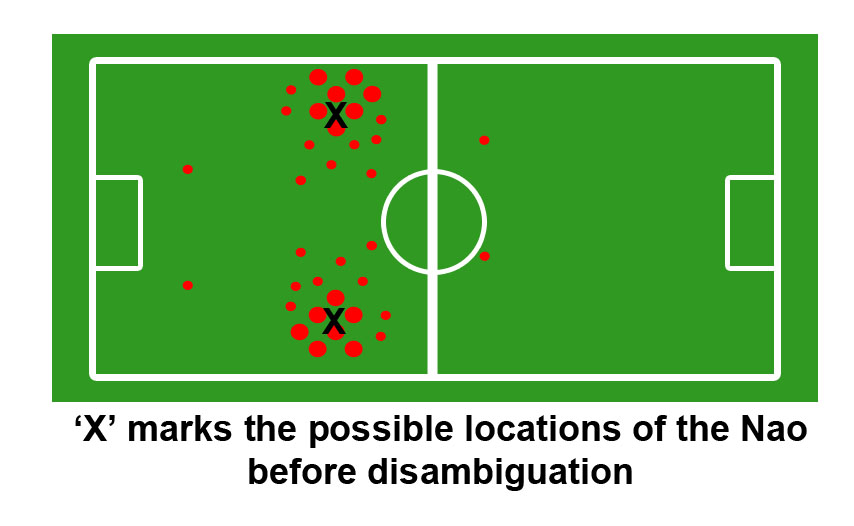
\includegraphics[width=0.6\textwidth]{../Drawings/localisation/beforeDisambiguate.jpg}
    \caption{Two possible positions are surrounded by particles with large weights.} 
    \label{fig:before}
\end{minipage}
\begin{minipage}[b]{0.5\linewidth}
  \centering
    \includegraphics[width=0.5\textwidth]{../Drawings/localisation/NaoField.jpg}
    \caption{The SimRobot simulation of the particles on re-entering the field}
    \label{fig:beforeSim}
\end{minipage}
\end{figure}


%Disambiguation step
%Discuss when it comes onto the field.
\section{Descriptor Matching}
\label{sec:disambiguation}
It is at this point that the proposed modification to the localisation algorithm will be utilised. It should be noted that each particle has an $(x,y)$ position and an orientation $\theta$. It is the particle's orientation $\theta$ that is crucial to this algorithm working effectively. As can be seen in \figref{fig:penaltyOver}, the robot has re-entered the field and the particles are given random orientations. The robot will then rotate its head counter-clockwise (arbitrarily chosen) to face the left goal post as shown in \figref{fig:turnedLeft}. Both clusters of particles will rotate counter-clockwise by the same angle. Due to the symmetry of the environment, the correct cluster will rotate in the same direction as the robot's head whereas the incorrect cluster will rotate in the opposite direction.\\

The robot will then utilise its feature extraction algorithm to identify interest points in regions behind the respective goal post that it is facing. This scenario is shown in \figref{fig:featureMatching} where the robot has identified interest points $F1, F2, F3$. Descriptors for these interest points will then be computed and the set of descriptors will be referred to as $d_{current}^c$ where $c$ is the current image.

The algorithm will then match the current descriptors from $d_{current}^c$ with descriptors from $d_{initial}^j|j=1,2...m$. The set of descriptors $d_{initial}^j$, corresponding to the best match with $d_{current}^c$, will determine the goal post which the robot is currently facing. This can be seen in the figure whereby the robot has matched its current descriptors to the stored descriptors relating to the image of the robot's goal post. In this example, the robot knows from matching the descriptors that it is therefore facing its team's goalpost.\\
 
\begin{figure}[ht!]
\begin{minipage}[b]{0.5\linewidth}
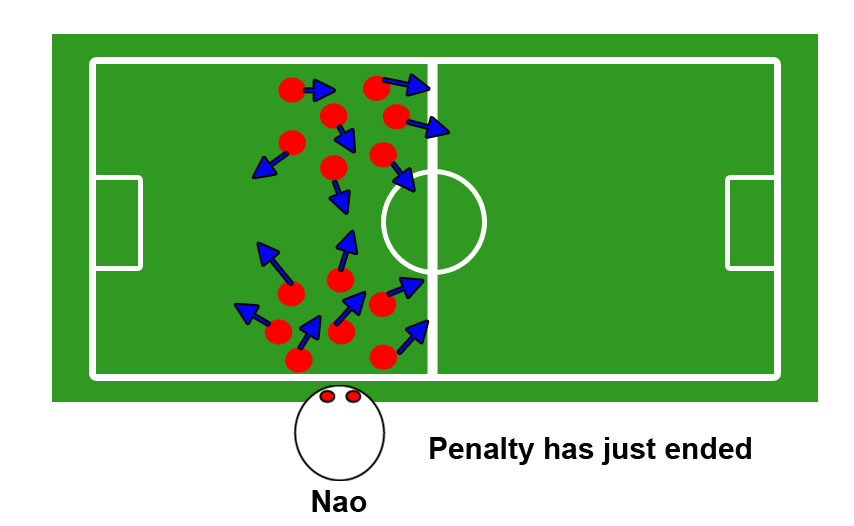
\includegraphics[scale=0.2]{../Drawings/localisation/localisationAlgorithmPenaltyEnded.jpg}
\caption{The particles representing hypotheses of the possible robot position after the robot has served its penalty time.}
\label{fig:penaltyOver}
\end{minipage}
\hspace{0.5cm}
\begin{minipage}[b]{0.5\linewidth}
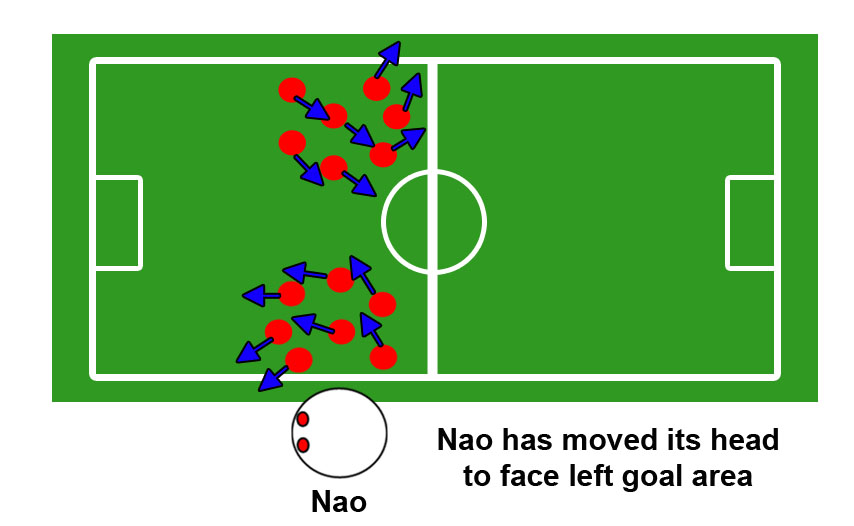
\includegraphics[scale=0.2]{../Drawings/localisation/localisationAlgorithmTurnedLeft.jpg}
\caption{The robot turns its head to the left and the orientations of the particles change accordingly.}
\label{fig:turnedLeft}
\end{minipage}
\end{figure}

%Matching interest point descriptors
\begin{figure}[h!] 
  \centering
    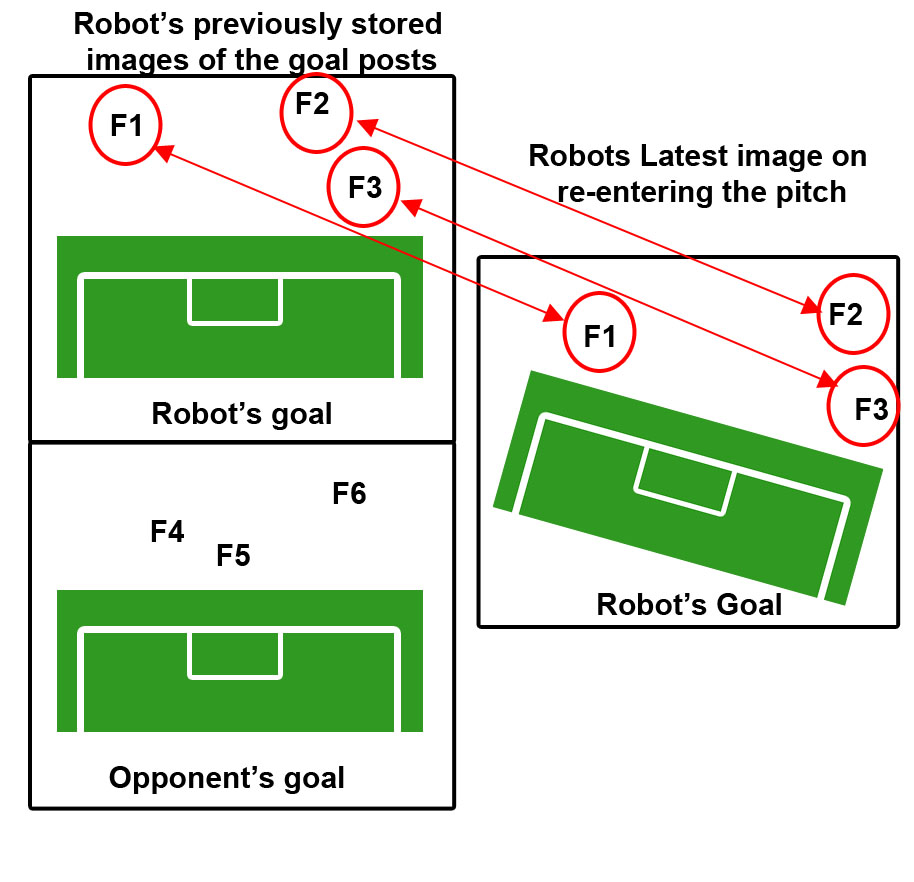
\includegraphics[width=0.5\textwidth]{../Drawings/localisation/featureMatching.jpg}
    \caption{Matching interest point descriptors to disambiguate the robot's position}
    \label{fig:featureMatching}
\end{figure}



\section{Re-weighting Procedure}
\label{sec:reweighting}
The algorithm will be able to disambiguate the robots position on the field by re-weighting the particles in the AMCPF algorithm. The re-weighting procedure is performed as follows. The algorithm knows the robots current head orientation $\beta$. All particles whose current orientation is $\beta -\frac{\pi}{2} \leq \theta \leq \beta + \frac{\pi}{2}$ will be assigned a large weight as these particles are most likely clustered around the robot's true position. All other particles will be assigned a low weight. This should result in the robot being able to disambiguate its position as seen in \figref{fig:reweight}. Once this has been achieved, the AMCPF algorithm returns to its normal operation which only re-weights particle using visual landmarks shown in \figref{fig:localiseLandmarks}. If some incorrect particles are assigned large weights, then they will quickly disappear in subsequent re-weighting procedures since the particle's position and orientation hypothesis will not coincide with the observations that the robot receives from the field.\\


%Leading up to the final state
\begin{figure}[h!] 
\centering
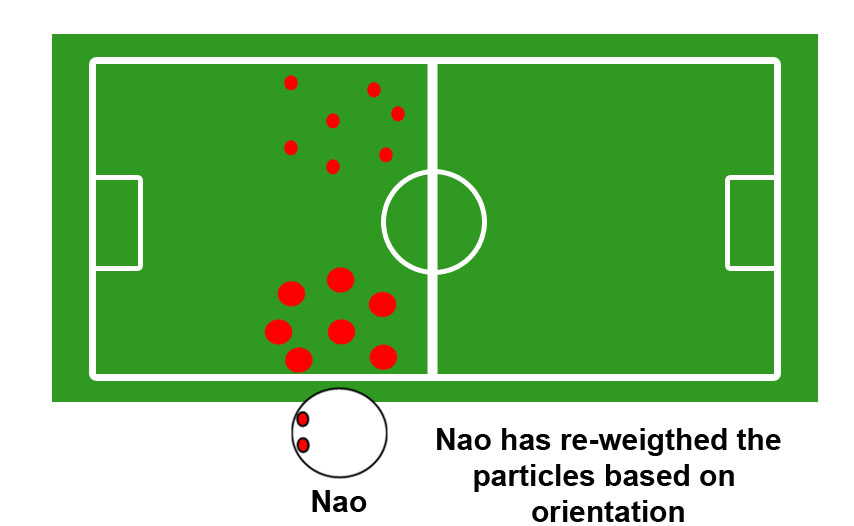
\includegraphics[scale=0.2]{../Drawings/localisation/localisationAlgorithmReweight.jpg}
\caption{The robot then re-weights the particles that have approximately the same orientation as the robot.}
\label{fig:reweight}
\end{figure}

%The final state
%\begin{figure}[h!] 
%  \centering
%    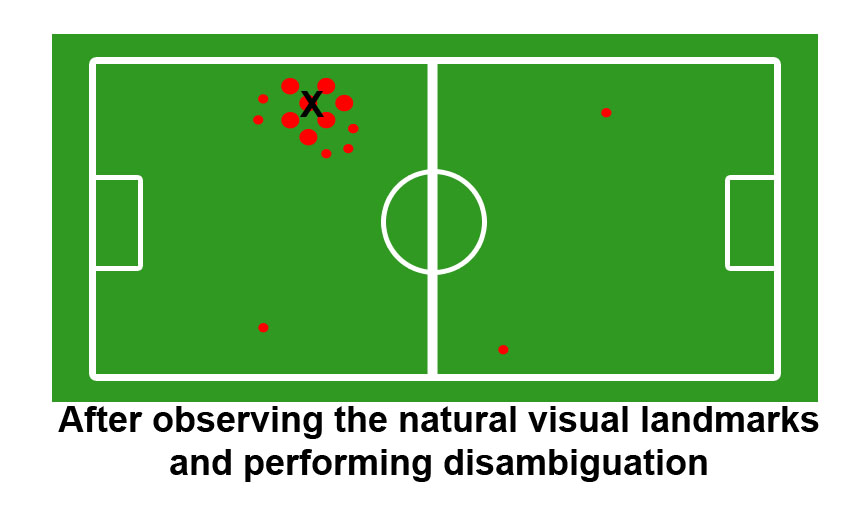
\includegraphics[width=0.5\textwidth]{../Drawings/localisation/afterDisambiguate.jpg}
%    \caption{The robot's estimated position after disambiguation}
%    \label{fig:after}
%\end{figure}




%Discuss how the robot performs the localisation procedure.
%Briefly mention the fact that the robot relocalises itself using a re-weighting routine
%
%\section{Re-weighting Particles and Importance Sampling}
%\label{sec:reweighting}
%This is where the orientation algorithm is placed



%\section{Bhuman Code Structure}
%\label{sec:codeStructure}
%Discuss the basics of the bhuman code structure
%Include a basic diagram of modules, representations etc

%\section{Natural Landmark Code Structure}
%\label{sec:naturalLandmarkCode}
%Discuss how the Natural landmark detection has been placed into the bhuman code structure
%include a diagram from the simRobot interface

%\section{Summary}
%\label{sec:summary4}
\chapter{Experiments and Results}
\label{sec:experimentsResults}
This section aims to determine which feature extraction algorithm exhibits the best  computational performance and matching accuracy. Computational performance involves comparing the algorithms based on the time taken to detect interest points, computing the interest point descriptors and matching the descriptors using the matching techniques mentioned in \secref{sec:matchingTechniques}. Matching accuracy is defined in this context as the ability of the algorithm to determine whether or not a pair of images \textit{overlap} and hence match one another. The criteria defining a pair of overlapping images is detailed in \secref{sec:datasets}.\\

All experiments were performed using a laptop with an Intel Core 2 Duo T6400 $2.00$GHz processor. The Nao robot for which these algorithms have been designed uses an ATOM Z530 $1.6$GHz processor \citep{NaoHead}. Thus, the computational times presented in this chapter are faster than the times expected on the Nao. In addition to this, the Nao's camera can process $30$ Frames Per Second (FPS) meaning that the feature extraction algorithm must be able to perform a detection, extraction and matching routine in under $33$ ms. This will enable the Nao to process every image which is crucial to obtaining robust, real-time matching performance. \\

The experiments were conducted on a variety of feature extraction and matching algorithms. The feature extraction algorithms tested and compared in these experiments are BRISK0, BRISK, BRISK0-U-BRISK, BRISK0-SURF2D and 1D SURF. There are three types of matching techniques utilised for these experiments. They are 2-Nearest Neighbors, Radius Matching and RANSAC as described in \secref{sec:matchingTechniques}. Both 2-Nearest Neighbors and Radius Matching have been implemented on all of the BRISK-based feature extraction algorithms. This includes all algorithms that use BRISK0 or BRISK feature detectors and/or descriptors. 1D SURF utilises RANSAC matching which has been previously implemented by the \textit{rUNSWift} team \citep{Anderson}. This implementation has been used for the experiments in this section.\\ 

%The algorithms are run in a variety of different environments as will be discussed in \secref{sec:datasets}. The main image datasets are those captured in the \textit{Main Robocup Environment}. Since the immediate focus of this project is on developing a robust feature extraction technique on the Nao robot for the purpose of Robocup, the above-mentioned environment  and its corresponding datasets are most relevant and will therefore be the core focus of the experiments.\\

Parameters $p$ in this chapter correspond to the various thresholds required for detecting interest points and determining matches. The parameters used for each method are shown in \tabref{tab:parameters}. The Minimum Interest Point Detection Threshold (MIPDT) is the threshold above which a pixel is detected as an interest point. The Maximum Accepted Hamming Distance (MAHD) is the maximum number of bits that can differ when comparing two feature descriptors, below which the descriptors are to be considered a match. The Maximum Accepted Euclidean Distance (MAED) is the maximum euclidean distance below which two feature descriptors are considered to be a match.\\

\begin{table}
\centering
\caption{The parameters evaluated for each feature extraction algorithm}
\begin{tabular}{|c|c|c|}
\hline 
Method & Parameter 1 & Parameter 2\tabularnewline
\hline 
 & \multicolumn{2}{c|}{2-Nearest Neighbors Matching}\tabularnewline
\hline 
BRISK0 & MIPDT & N/A\tabularnewline
\hline 
BRISK4 & MIPDT & N/A\tabularnewline
\hline 
BRISK0 SURF2D & MIPDT & N/A\tabularnewline
\hline 
BRISK0 - UBRISK & MIPDT & N/A\tabularnewline
\hline 
 & \multicolumn{2}{c|}{Radius Matching}\tabularnewline
\hline 
BRISK0 & MIPDT & MAHD\tabularnewline
\hline 
BRISK4 & MIPDT & MAHD\tabularnewline
\hline 
BRISK0 SURF2D & MIPDT & MAED\tabularnewline
\hline 
BRISK0 - UBRISK & MIPDT & MAHD\tabularnewline
\hline 
\end{tabular}
\label{tab:parameters}
\end{table}

This chapter will be developed as follows. Initially the optimal parameters for each of the feature extraction algorithms will be calculated using a score function that I developed. Using these parameters, various matching properties will be verified which includes verification of the 2-NN ratio constraint mentioned in \secref{sec:matchingTechniques}. The Image Matching Score (IMS) will be defined and used to determine how well two images match one another. Some potentially useful properties regarding interest points have been identified and will be discussed. Following this, the feature extraction algorithms will then use these optimal parameters in order to match pairs of images on datasets in different environments. The best algorithm to be used on the Nao robot will then be determined.\\   


\section{The Main Robocup Environment}
\label{sec:datasets}
The \textit{Main Robocup Environment} has been used extensively in experiments throughout this chapter and the image datasets generated from this environment need to be detailed.\\

Four image datasets are generated in this environment for each experiment. The images in these datasets have been captured using the Nao's upper camera. The Nao's camera is focused on the regions behind the goalposts. The first set of goalposts will be referred to as the Player's Goal (PG). The second set of goalposts will be referred to as the Opponents Goal (OG) as seen in \figref{fig:datasetSetup}. \\


\begin{figure}%[ht!]
  \centering
    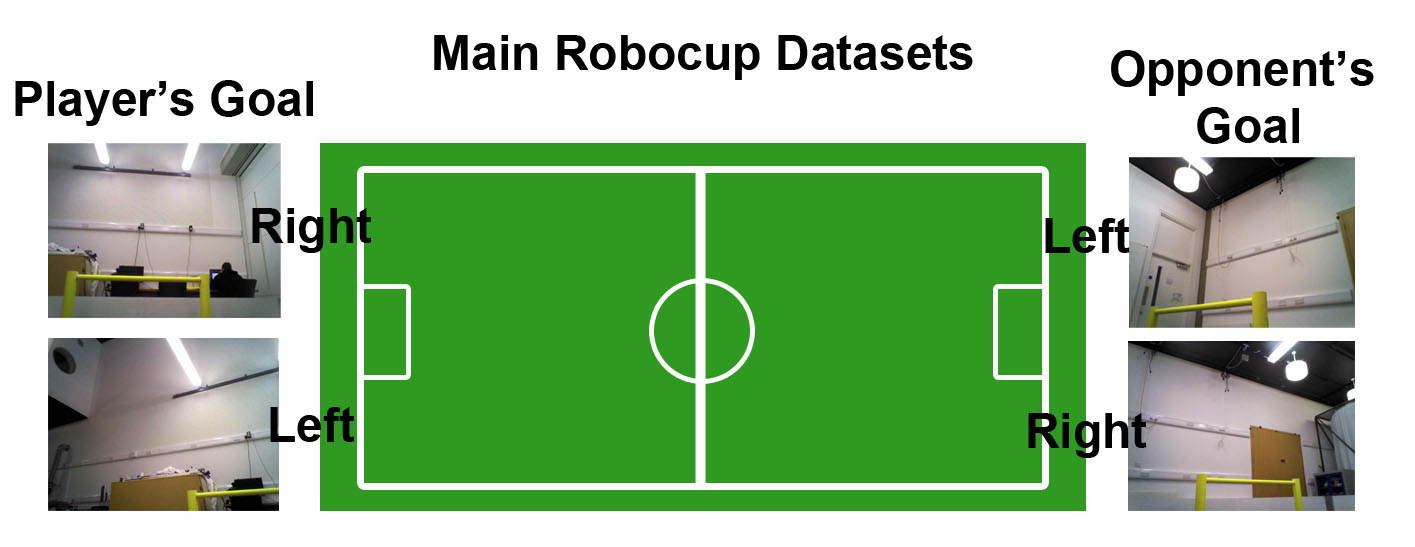
\includegraphics[width=1.0\textwidth]{../Drawings/RobocupDataset/DatasetSetup.jpg}
    \caption{The Robocup field setup and typical images corresponding to regions behind each respective goal} 
    \label{fig:datasetSetup}
 \end{figure}


As can be seen in the figure, the first dataset is of the area to the left of the player's goal (\textit{PG Left}). The second dataset is to the right of the player's goal (\textit{PG Right}). The third dataset is to the left of the opponent's goal (\textit{OG Left}). The fourth dataset is to the right of the opponents goal (\textit{OG Right}). The abbreviations, shown in braces, will be used to refer to these datasets for the remainder of this chapter. Typical images from each of these datasets are shown in \figref{fig:dataset1} to \figref{fig:dataset4} respectively.\\

\begin{figure}[h!]
\begin{minipage}[b]{0.5\linewidth}
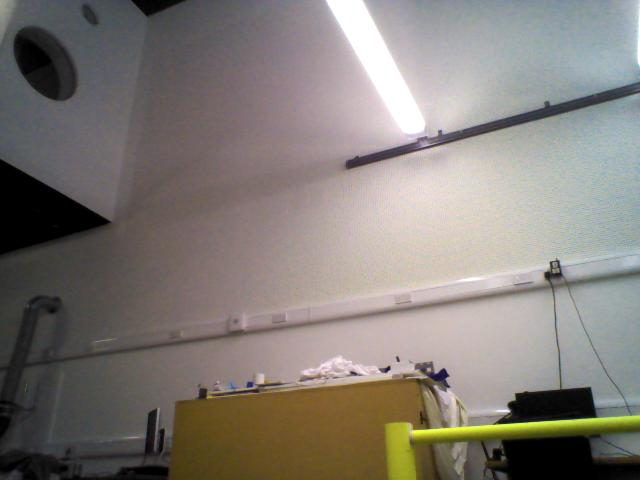
\includegraphics[scale=0.4]{../Drawings/datasetImages/mgLeft.jpg}
\caption{Dataset one showing an image from \textit{PG Left}}
\label{fig:dataset1}
\end{minipage}
\hspace{0.5cm}
\begin{minipage}[b]{0.5\linewidth}
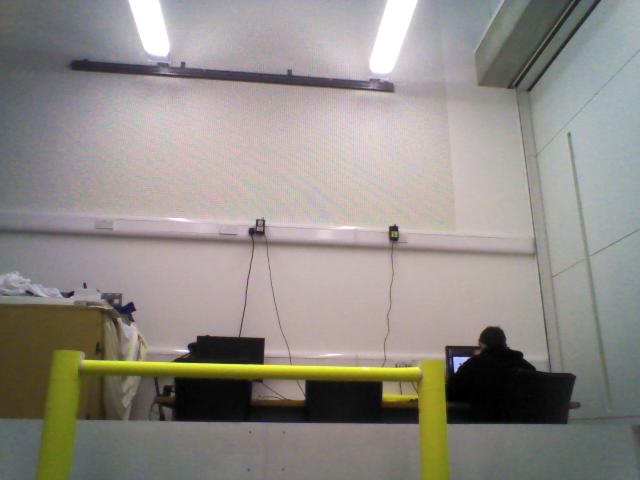
\includegraphics[scale=0.4]{../Drawings/datasetImages/mgRight.jpg}
\caption{Dataset two showing an image from \textit{PG Right}}
\label{fig:dataset2}
\end{minipage}
\hspace{0.5cm}
\begin{minipage}[b]{0.5\linewidth}
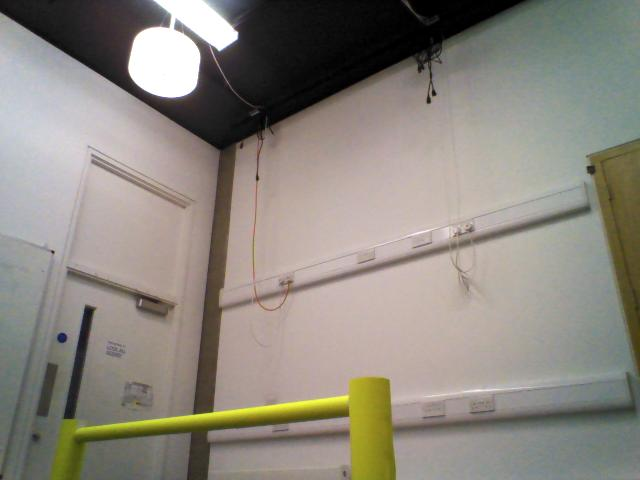
\includegraphics[scale=0.4]{../Drawings/datasetImages/ogLeft.jpg}
\caption{Dataset three showing an image from \textit{OG Left}}
\label{fig:dataset3}
\end{minipage}
\hspace{0.5cm}
\begin{minipage}[b]{0.5\linewidth}
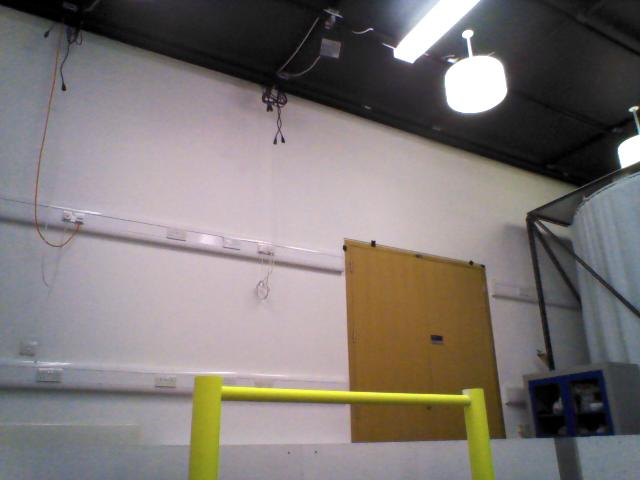
\includegraphics[scale=0.4]{../Drawings/datasetImages/ogRight.jpg}
\caption{Dataset four showing an image from \textit{OG Right}}
\label{fig:dataset4}
\end{minipage}
\end{figure}

Pairs of images taken from the same dataset are referred to as overlapping images. A pair of images are considered to overlap one another if at least $50\%$ of the first image visually overlaps the second image. This has been manually performed to ensure that the images do indeed overlap. Pairs of images with no overlap, taken from different datasets, are referred to as non-overlapping images. In order to ensure that images do not overlap, datasets from opposite sides of the football field were compared. Thus datasets \textit{PG Left} and \textit{PG Right} have been separately compared with datasets \textit{OG Left} and \textit{OG Right} respectively. Generating overlapping and non-overlapping image pairs has therefore been achieved by combining datasets as shown in \tabref{table:overlap}. If the same dataset appears in both columns in the table, then images within the same dataset are compared to one another generating overlapping image pairs. \\

It must be noted that for clarity, the terms \textit{match} and \textit{interest point match} will be used interchangeably to refer to a match between a pair of interest points. An \textit{image match} and \textit{overlap} will be used interchangeably to refer to a match between a pair of images indicating an overlapping image pair.\\

\begin{table}
\centering
\caption{Combinations of datasets used to generate overlapping and non-overlapping image pairs in the \textit{Main Robocup Environment}}
\begin{tabular}{|c|c|}
\hline 
\textbf{Dataset A} & \textbf{Dataset B}\tabularnewline
\hline 
\hline 
\multicolumn{2}{|c|}{\textbf{Overlapping Images}}\tabularnewline
\hline 
MG LEFT & MG LEFT\tabularnewline
\hline 
MG RIGHT & MG RIGHT\tabularnewline
\hline 
OG LEFT & OG LEFT\tabularnewline
\hline 
OG RIGHT & OG RIGHT\tabularnewline
\hline 
\multicolumn{2}{|c|}{\textbf{Non-Overlapping Images}}\tabularnewline
\hline 
MG LEFT & OG LEFT\tabularnewline
\hline 
MG LEFT & OG RIGHT\tabularnewline
\hline 
MG RIGHT & OG LEFT\tabularnewline
\hline 
MG RIGHT & OG RIGHT\tabularnewline
\hline 
\end{tabular}
\label{table:overlap}
\end{table}

The \textit{Main Robocup Environment} has been used as the test environment in \secref{sec:optimalParameters}, \secref{sec:matchingProperties} and \secref{sec:matchingStats}. Four image datasets of regions behind the Robocup goalposts have been captured specifically for the experiments in these sections and will be referred to as the \textit{Main Robocup Parameter Datasets}. In total, these datasets collectively contain $108$ overlapping images which have been used to generate $1421$ overlapping image pairs. This is achieved by pairing all combinations of images without repetition in each image dataset. A further $108$ non-overlapping images have been used to generate $2808$ non-overlapping image pairs. The combinations of the various datasets and the number of image pairs generated are shown in \tabref{tab:mrpd}. \\

\begin{table}
\centering
\caption{Overlapping and non-overlapping image pairs generated from the \textit{Main Robocup Parameter Datasets} }
\begin{tabular}{|c|c|c|c|c|}
\hline 
\textbf{Dataset A} & \textbf{Dataset B} & \textbf{Images in A} & \textbf{Images in B} & \textbf{Image Pairs}\tabularnewline
\hline 
\hline 
\multicolumn{5}{|c|}{\textbf{Overlapping Images}}\tabularnewline
\hline 
MG LEFT & MG LEFT & 26 & 26 & 325\tabularnewline
\hline 
MG RIGHT & MG RIGHT & 28 & 28 & 378\tabularnewline
\hline 
OG LEFT & OG LEFT & 31 & 31 & 465\tabularnewline
\hline 
OG RIGHT & OG RIGHT & 23 & 23 & 253\tabularnewline
\hline 
 & \textbf{Total} & 108 & 108 & 1421\tabularnewline
\hline 
\multicolumn{5}{|c|}{\textbf{Non-Overlapping Images}}\tabularnewline
\hline 
MG LEFT & OG LEFT & 26 & 31 & 780\tabularnewline
\hline 
MG LEFT & OG RIGHT & 26 & 23 & 572\tabularnewline
\hline 
MG RIGHT & OG LEFT & 28 & 31 & 840\tabularnewline
\hline 
MG RIGHT & OG RIGHT & 28 & 23 & 616\tabularnewline
\hline 
 & \textbf{Total} & 108 & 108 & 2808\tabularnewline
\hline 
\end{tabular}
\label{tab:mrpd}
\end{table}

%Throughout this chapter, the term \textit{Image Match} refers to whether or not two images overlap one another. A matching of individual interest point descriptors in corresponding images will be referred to as a \textit{Match}.\\
\section{Calculating the Optimal Feature Extraction Parameters}
\label{sec:optimalParameters}
This section describes the calculation of the optimal parameters for each of the feature extraction algorithms. As mentioned previously, these parameters are calculated in the \textit{Main Robocup Environment} and utilise the \textit{Main Robocup Parameter Datasets}. The parameters are the MIPDT, MAHD and MAED as shown in \tabref{tab:parameters}. The 1D SURF implementation does not undergo this procedure since the recommended parameter settings by \citet{Anderson} have been used to perform the subsequent experiments.\\

%Describes how to find the optimal hamming distance, euclidean distance, and response thresholds for each method
The procedure used to determine the optimal parameters for each of the feature extraction algorithms will now be detailed. The four image datasets, \textit{MG LEFT}, \textit{MG RIGHT}, \textit{OG LEFT} and \textit{OG RIGHT}, containing in total $108$ overlapping images, were used to determine the optimal parameter values. All possible combinations of overlapping image pairs were compared in each of the four datasets, without repetition, for various parameter values which will be mentioned below. \\

For each image pair, the Single Image Score (SIS) needs to be computed. This equation is shown in \eqnref{eqn:optimalParameters}. The SIS represents how well a pair of images, $i_1, i_2$, overlap one another in a particular dataset $d$, for a particular Feature Extraction algorithm $FE$, using a certain set of parameters, \textbf{p}. For example, if the feature extraction algorithm used is BRISK0, then the $SIS_{(i_1, i_2), d}^{BRISK0, \textbf{p}}$ presents the SIS score for the pair of images $i_1, i_2$ for specific MIPDT and MAHD values \textbf{p}, in a particular dataset $d$. \\

\begin{equation}
SIS_{(i_1, i_2), d}^{FE, \textbf{p}} = \alpha f(t_{i_1,i_2}) + (1-\alpha) g(\textit{NVM}_{i_1,i_2}) \quad 0 \leq \alpha \leq 1
\label{eqn:optimalParameters}
\end{equation}

This SIS score is composed of two normalised scoring functions, namely $f(t_{i_1, i_2})$ and $g(NVM_{i_1, i_2})$ shown in \eqnref{eqn:time} and \eqnref{eqn:nvm} respectively. $f(t_{i_1, i_2})$ represents the timing score for a pair of images $i_1, i_2$ for a particular dataset based on the overall time $t$, taken to perform the image processing, detection, extraction and matching routines respectively between these images. The unit of $t$ is milliseconds and the value of $t$ is normalised to a scale between $0$ and $1$. This is achieved by multiplying $t$ by $0.9$ and dividing this result by $t_{max}$ where $t_{max}$ is the largest time tabulated for the current dataset $d$ in milliseconds. A value of $0.1$ is then added to this ratio in order to  prevent $log(0) = \infty$ which would largely bias the results as well as ensuring that the value $(\frac{0.9 t}{t_{max}} + 0.1)$ is normalised between $0$ and $1$. The function $f(t_{i_1, i_2})$ will ensure that, for large $t$, meaning that the algorithm takes a large amount of time to perform the routine, the timing score will be low, whereas for small $t$ the timing score will be high. \\

The second scoring function used to calculate the SIS score is $g(NVM_{i_1, i_2})$. This scoring function rewards a pair of images $i_1, i_2$ if they contain a large amount of valid interest point matches. This is intuitive as the more valid matches there are between two images, the more certain it is that the pair of images overlap one another. The variable $NVM$ represents the Number of Valid Matches (NVM) between two images. This function is normalised between $0$ and  $1$ by dividing this variable by the total amount of matches, $M_{total}$, generated from the pair of images $i_1, i_2$. The reason $M_{total}$ has been chosen as the normalisation factor is because it prevents a biased score. A biased score can occur in the following scenario. Assume that a pair of images $a_1, a_2$ generate a large amount of matches, but only a small proportion of these matches are valid. This is in contrast to another pair of images $b_1, b_2$ from the same dataset that generated a small set of matches, but a high proportion of valid matches. If $M_{total}$ was denoted as the maximum number of matches in the dataset, then images $b_1, b_2$ would have a smaller score than that of $a_1, a_2$ even though $b_1, b_2$ has a higher proportion of valid matches. Thus $M_{total}$ has been chosen to be the total number of matches between a pair of images $i_1, i_2$. This relative value largely prevents the biased scores. The value $\epsilon$ has been added to ensure that no infinite scores are computed. $\epsilon$ can take any value greater than $0$ and has been chosen to have a value of $0.1$, based on observation, for these experiments.\\ 

The parameter $\alpha$ is a weight that is used to bias the effects of the two scoring functions. Thus it can be used as a control to determine whether time or the number of valid matches should have a larger influence on the SIS. $\alpha$ is defined between $0$ and $1$. For these experiments, $\alpha$ was set to $0.6$. This value has been chosen as a slight bias towards more computationally efficient algorithms is desired. This is because computational performance is a crucial aspect of the algorithm if it is to be implemented on the Nao robot.\\

\begin{equation}
f(t_{i_1, i_2}) = \mid log_{10}(\frac{0.9 t_{i_1, i_2}}{t_{max}^{FE}} + 0.1) \mid \quad f(t_{i_1, i_2})\in [0, 1]
\label{eqn:time}
\end{equation}

\begin{equation}
g(NVM_{i_1, i_2}) = \frac{NVM_{i_1, i_2}}{M_{total, (i_1, i_2)} + \epsilon} \quad g(NVM_{i_1, i_2}) \in [0, 1] %State that epsilon is between 0 and 1
\label{eqn:nvm}
\end{equation}

Once the SIS score has been calculated for each pair of images $i_1, i_2$, these scores are then summed together for a particular set of parameter values \textbf{p} using a specific feature extraction algorithm $FE$ in a particular dataset $d$. The resulting score is called the Multi-Image Score (MIS) and is shown in \eqnref{eqn:mims}.\\



\begin{equation}
MIS_{\textbf{p}, d}^{FE} = \beta \tau + (1-\beta) h(\textit{IZM}) \quad 0 \leq \beta \leq 1
\label{eqn:mims}
\end{equation}

\begin{equation}
\tau = \frac{\sum_{i_1, i_2=1 , i_1 \neq i_2}^{N} \textit{SIS}_{(i_1, i_2),d}^{FE,\textbf{p}}}{N}
\label{eqn:tau}
\end{equation}

The first term of the MIS score is the computation of the mean of all SIS scores for a particular set of parameter values \textbf{p}, using a specific feature extraction algorithm $FE$, in a particular dataset $d$. This value is referred to as $\tau$ and is shown in \eqnref{eqn:tau}.\\

The second term is a scoring function that accounts for the number of Image Zero Matches (\textit{IZM}) for a particular set of parameter values. An \textit{IZM} is defined as a pair of images containing no valid interest point matches. The function $h(IZM)$, defined in \eqnref{eqn:izm}, determines the number of \textit{IZMs} in a particular dataset $d$, for a particular set of parameter values \textbf{p} using feature extraction algorithm $FE$. This equation has the same form as equation \eqnref{eqn:time} and therefore behaves in the same way. However, in this case the denominator $\textit{IZM}_{max}^{FE}$ represents the maximum number of IZMs found for a particular parameter setting in a particular dataset using a particular feature extraction algorithm. This function therefore penalises parameter settings that result in a large number of \textit{IZM}s since \textit{IZM}s should not be present in a dataset of overlapping images. \\

\begin{equation}
h(\textit{IZM})_{\textbf{p}, d}^{FE} = \mid log_{10}(\frac{0.9\textit{IZM}_{\textbf{p}}^{FE}}{\textit{IZM}_{max}^{FE}} + 0.1) \mid \quad h(\textit{IZM}_{p}^{FE})\in [0, 1]
\label{eqn:izm}
\end{equation}

The MIS score contains a weighting parameter $\beta$ that can again be used to control the influence of each term in the function. $\beta$, like $\alpha$, is again between $0$ and $1$. $\beta$ has been set to a value of $0.6$. This creates a slight bias towards feature extraction algorithms that are computationally efficient and have many valid interest point matches. \\

\eqnref{eqn:mims} therefore provides an overall score of how well image pairs overlap one another, for a specific setting of parameter values \textbf{p} in dataset $d$ using feature extraction algorithm $FE$. \\

The \textit{Main Robocup Parameter Datasets} consist of four image datasets and thus  optimal parameter values are generated for each specific dataset. In order to determine the best overall set of parameters for each feature extraction algorithm $FE$, over all datasets, two methods were utilised. The first involved finding the maximum $\textit{MIS}_{(\textbf{p}, d)}^{FE}$ score for each dataset $d$, for a particular feature extraction algorithm $FE$, as well as the corresponding parameter values \textbf{p} that generated this \textit{MIS} score. Since there are four datasets, four sets of parameters are generated. These parameters are then averaged as shown in \eqnref{eqn:average}, and the resulting parameter values are set as the optimal parameters, $\textbf{p}^*$ for the feature extraction algorithm. Here, $d_i$ represents the $i^{th}$ dataset.\\

\begin{equation}
\textbf{p}^* = mean( max(p_{d_1}), max(p_{d_2}), max(p_{d_3}) ...) \quad d = 1,2...m
\label{eqn:average}
\end{equation}

This methodology does not necessarily produce the best set of optimal parameters. The second technique does not initially take the maximum \textit{MIS} score but first averages all corresponding \textit{MIS} scores across all datasets. A corresponding \textit{MIS} score is defined as a score that has been generated from the same parameter values but in a different dataset. Once all \textit{MIS} scores have been averaged across all datasets, a vector of \textit{MIS} scores results. The maximum \textit{MIS} score is then determined from this vector. This has the advantage of finding the most consistent score across all datasets rather than finding the maximum \textit{MIS} score separately for each dataset.\\

The first technique will be referred to as the \textit{Maximum Parameter Setting} (MPS). The second technique will be referred to as the \textit{Consistent Parameter Setting} (CPS).\\

Graphs showing the parameters for the CPS settings are presented in \figref{fig:BRISK0knnOptimal} to \figref{fig:BRISK0UBRISKHammingOptimal} respectively. The optimal parameter value(s) corresponding to these settings are indicated by the red lines. This has been performed for both the 2-NN and Radius Matching techniques respectively. Since the MPS settings are determined by finding the mean of four maximums as shown in \eqnref{eqn:average} from each dataset, graphs were not computed for this setting.\\

%Could possibly add in the addition of averaging the mScore matrices and then finding the maximum value. The advantage of this is to find the most consistent radius and threshold.  

%The optimal parameter graphs
\begin{figure}
\begin{minipage}[b]{0.5\linewidth}
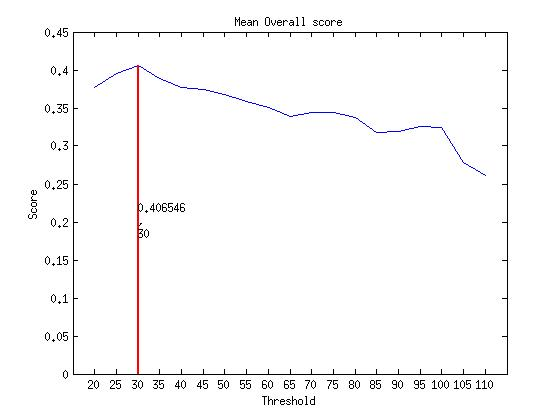
\includegraphics[scale=0.4]{../Drawings/OptimalParameters_SBRISK_SBRISK_KNN.jpg}
\caption{The optimal parameters for BRISK0 with 2-NN Matching}
\label{fig:BRISK0knnOptimal}
\end{minipage}
\hspace{0.5cm}
\begin{minipage}[b]{0.5\linewidth}
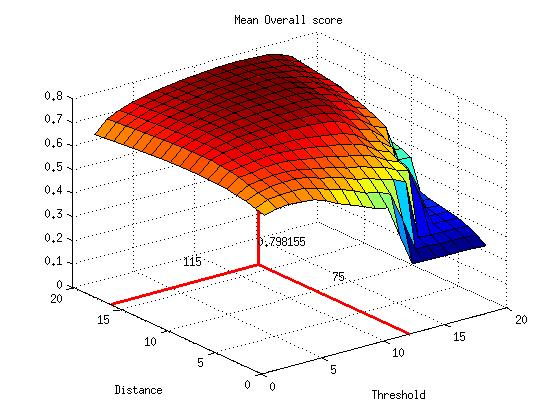
\includegraphics[scale=0.4]{../Drawings/OptimalParameters_SBRISK_SBRISK_hamming.jpg}
\caption{The optimal parameters for BRISK0 with Radius Matching}
\label{fig:BRISK0hammingOptimal}
\end{minipage}
\begin{minipage}[b]{0.5\linewidth}
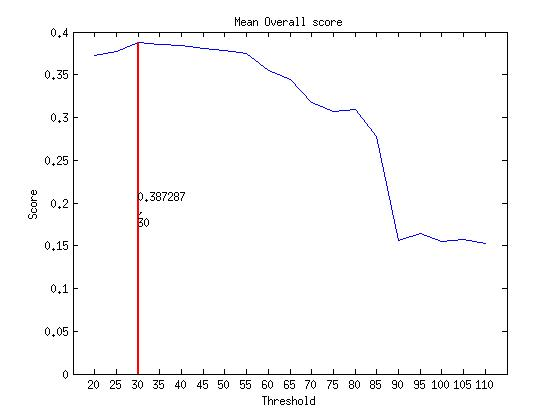
\includegraphics[scale=0.4]{../Drawings/OptimalParameters_BRISK4_BRISK4_KNN.jpg}
\caption{The optimal parameters for BRISK with 2-NN Matching}
\label{fig:BRISKknnOptimal}
\end{minipage}
\begin{minipage}[b]{0.5\linewidth}
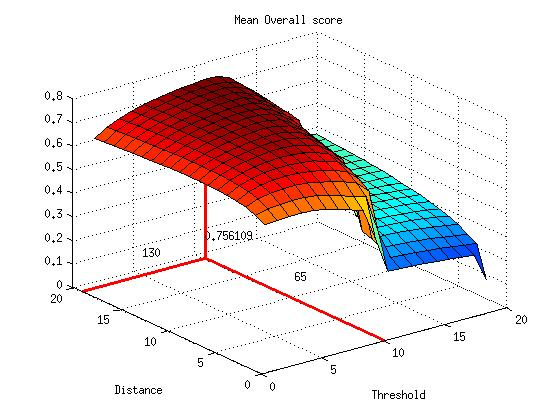
\includegraphics[scale=0.4]{../Drawings/OptimalParameters_BRISK4_BRISK4_Hamming.jpg}
\caption{The optimal parameters for BRISK with Radius Matching}
\label{fig:BRISKhammingOptimal}
\end{minipage}
\end{figure}

\begin{figure}
\begin{minipage}[b]{0.5\linewidth}
\includegraphics[scale=0.4]{../Drawings/OptimalParameters_SBRISK_SURF2D_KNN.jpg}
\caption{The optimal parameters for BRISK0 SURF2D with 2-NN Matching}
\label{fig:BRISK0surfknnOptimal}
\end{minipage}
\hspace{0.5cm}
\begin{minipage}[b]{0.5\linewidth}
\includegraphics[scale=0.4]{../Drawings/OptimalParameters_SBRISK_SURF2D_Hamming.jpg}
\caption{The optimal parameters for BRISK0 SURF2D with Radius Matching}
\label{fig:BRISK0surfHammingOptimal}
\end{minipage}
\begin{minipage}[b]{0.5\linewidth}
\includegraphics[scale=0.4]{../Drawings/OptimalParameters_SBRISK_UBRISK_KNN.jpg}
\caption{The optimal parameters for BRISK0 - U-BRISK with 2-NN Matching}
\label{fig:BRISK0UBRISKknnOptimal}
\end{minipage}
\begin{minipage}[b]{0.5\linewidth}
\includegraphics[scale=0.4]{../Drawings/OptimalParameters_SBRISK_UBRISK_Hamming.jpg}
\caption{The optimal parameters for BRISK0 - U-BRISK with Radius Matching}
\label{fig:BRISK0UBRISKHammingOptimal}
\end{minipage}
\end{figure}

These experiments produced a set of optimal parameters that were generated for both the MPS and CPS parameter settings. The parameter settings are shown in \tabref{tab:knnStatistics} and \tabref{tab:hammingStatistics} for each respective matching technique. For the 2-NN tests, only the Minimum Interest Point Detection Threshold (MIPDT) parameter was varied in the range $20 \rightarrow 115$ in increments of $5$. For the Radius Matching tests, both the MIPDT and the MAHD/MAED threshold parameters were varied. The MIPDT was varied in the same range as the 2-NN tests. The MAHD is varied from $40 \rightarrow 135$ in increments of $5$ whereas the MAED is varied from $0.1 \rightarrow 0.28$ in increments of $0.01$.\\

As can be seen from the tables, the MPS parameter values tend to favour higher MIPDT thresholds compared to the CPS setting. This has the effect of detecting less interest points resulting in an increase in computational performance. In addition to this, lower MAHD/MAED values are also favoured by the MPS parameter setting which has the effect of producing less matches. In spite of these settings, a sufficient number of matches using the MPS setting are generated as will be shown in the sections to follow. This setting also increases the computational performance when computing matches between pairs of images.\\

Furthermore, both the MPS and CPS settings have been compared in three different environments as will be discussed in the sections to follow. It has been found that the MPS setting exhibits marginally better feature extraction performance in these environments. Based on this fact and since computational performance is a crucial aspect in developing a feature extraction algorithm that is suitable for real-time use on the Nao, the MPS setting will be used as the default setting for each of the relevant feature extraction algorithms. Therefore, the MPS setting is assumed to have generated the statistics unless otherwise stated in the sections to follow.\\

\begin{table}
\centering
\caption{The optimal thresholds for the 2-NN feature extraction algorithms}
\footnotesize
\begin{tabular}{|c|c|c|c|c|c|c|}
\hline 
Detector & Extractor & Matcher & $\alpha$ & $\beta$ & $MIPDT_{MPS}$ & $MIPDT_{CPS}$\tabularnewline
\hline 
\hline 
S-BRISK & S-BRISK & 2-NN & 0.6 & 0.6 & 46.25 & 30\tabularnewline
\hline 
BRISK4 & BRISK4 & 2-NN & 0.6 & 0.6 & 51.25 & 30\tabularnewline
\hline 
BRISK0 & SURF2D & 2-NN & 0.6 & 0.6 & 43.75 & 30\tabularnewline
\hline 
BRISK0 & UBRISK & 2-NN & 0.6 & 0.6 & 55 & 35\tabularnewline
\hline 
\end{tabular}
\label{tab:knnStatistics}
\end{table}

\begin{table}
\centering
\caption{The optimal thresholds for the Hamming/Euclidean distance feature extraction algorithms}
\footnotesize
\begin{tabular}{|c|c|c|c|c|c|c|c|c|}
\hline 
Detector & Extractor & Matcher & $\alpha$ & $\beta$ & $MIPDT_{MPS}$ & $MAHD_{MPS}$ & $MIPDT_{CPS}$ & $MAHD_{CPS}$\tabularnewline
 &  &  &  &  &  & $/MAED_{MPS}$ &  & $/MAED_{CPS}$\tabularnewline
\hline 
\hline 
S-BRISK & S-BRISK & Radius & 0.6 & 0.6 & 77.5 & 107.5 & 75 & 115\tabularnewline
\hline 
BRISK4 & BRISK4 & Radius & 0.6 & 0.6 & 80 & 120 & 65 & 130\tabularnewline
\hline 
BRISK0 & SURF2D & Radius & 0.6 & 0.6 & 65 & 0.28 & 60 & 0.28\tabularnewline
\hline 
BRISK0 & UBRISK & Radius & 0.6 & 0.6 & 75 & 121.25 & 75 & 130\tabularnewline
\hline 
\end{tabular}
\label{tab:hammingStatistics}
\end{table}

\section{Matching Properties}
\label{sec:matchingProperties}

\subsection{2-NN Matching Constraint}
\label{sec:knnMatchingConstraint}
In order to verify the 2-NN ratio constraint mentioned in \secref{sec:2nnMatching} and subsequently determine the optimum threshold for accepting valid interest point matches, a number of experiments were performed using the four BRISK-based feature extraction algorithms; namely BRISK0, BRISK, U-BRISK and BRISK0-SURF2D. 1D SURF is not utilised since it does not use the 2-NN ratio constraint for matching.\\

In order to generate invalid interest point matches, images with no overlap were compared, and any matches found during the comparison were flagged as invalid matches. This was performed on $2808$ non-overlapping image pairs from the \textit{Main Robocup Parameters Datasets}. To generate the valid interest point matches, $108$ identical image pairs from these datasets were compared and all matches found between these images were flagged as valid matches. An example of valid matches for two identical images are shown in \figref{fig:validKnn}.\\

 \begin{figure}%[ht!]
  \centering
    \includegraphics[width=1.0\textwidth]{../Drawings/knnRatio/KNN_ratio.jpg}
    \caption{An example of valid matches for 2-NN ratio. Only the first nearest neighbor is displayed for each interest point in this image.} 
    \label{fig:validKnn}
 \end{figure}

For both overlapping and non-overlapping images, 2-NN matching was performed generating two matches for every interest point. The distances in feature space of the first and second nearest neighbors from each interest point is then recorded. The ratio of these distances is then computed for both valid and invalid matches and the respective mean ratios are subsequently calculated. The results are shown in \tabref{tab:knnCriterion} for each of the four methods. As can be seen in the table, invalid matches have a mean ratio which is over $0.9$. Valid matches have a ratio of zero for BRISK-based descriptors and $0.0004$ for the SURF2D descriptor. A ratio of zero for the BRISK-based descriptors simply means that the hamming distance between the interest point descriptor and its first nearest neighbor in a corresponding image is zero. This is possible for identical image pairs as shown in \figref{fig:validKnn}.\\ 

This result illustrates a significant difference between the first and second nearest neighbors for valid and invalid matches. Based on this data, all matches whose 2-NN ratio is below $0.7$ are considered valid matches whereas all matches above $0.7$ are considered to be invalid matches. This value has been chosen based on the standard deviations shown in the table in order to ensure that the majority of 2-NN invalid matches are rejected. Graphs of the 2-NN ratio for both the BRISK0 - U-BRISK method and BRISK0 method are shown in \figref{fig:b0ubknnratio} and \figref{fig:b0knnratio} respectively. \\

\begin{figure}[h!]
\begin{minipage}[b]{0.5\linewidth}
\includegraphics[scale=0.4]{../Drawings/KNNRatio_SBRISK_UBRISK_20_60.jpg}
\caption{The 2-NN ratio for non-overlapping and overlapping images respectively using the BRISK0 - U-BRISK method}
\label{fig:b0ubknnratio}
\end{minipage}
\hspace{0.5cm}
\begin{minipage}[b]{0.5\linewidth}
\includegraphics[scale=0.4]{../Drawings/KNNRatio_SBRISK_SURF2D_20_60.jpg}
\caption{The 2-NN ratio for non-overlapping and overlapping images respectively using the BRISK0 method}
\label{fig:b0knnratio}
\end{minipage}
\end{figure}

In addition to this, the mean distance in feature space between the first and second nearest neighbor for each algorithm has been computed. It has been found that there is a significant difference between the distances for valid and invalid matches respectively. The mean distance could also be used as a global acceptance threshold but this is not generic and some feature descriptors may be more discriminatory than others \citep{Lowe2004}. This is evident in the case of BRISK0-SURF2D whose standard deviation is $68\%$ of the total mean distance for valid matches, indicating a huge amount of fluctuation about the mean. Thus the 2-NN ratio seems to be a more robust constraint than the mean distance in this scenario.\\

\begin{table}
\centering
\caption{The 2-NN Ratios}
\footnotesize
\begin{tabular}{|c|c|c|c|c|c|}
\hline 
\textbf{Method} & \textbf{Match Type} & \textbf{Mean 2-NN} & \textbf{Std } & \textbf{Mean Distance } & \textbf{Std }\tabularnewline
 &  & \textbf{ Ratio} & \textbf{Deviation} & \textbf{between 2-NN neighbors} & \textbf{Deviation}\tabularnewline
\hline 
\hline 
\textbf{BRISK0} & Invalid Matches & 0.94 & 0.06 & 7.45 & 7.58\tabularnewline
\hline 
 & Valid Matches & 0 & 0 & 97.66 & 37.97\tabularnewline
\hline 
\textbf{BRISK} & Invalid Matches & 0.93 & 0.06 & 7.93 & 7.91\tabularnewline
\hline 
 & Valid Matches & 0 & 0 & 86.47 & 42.78\tabularnewline
\hline 
\textbf{BRISK0 - UBRISK} & Invalid Matches & 0.94 & 0.05 & 7.78 & 7.58\tabularnewline
\hline 
 & Valid Matches & 0 & 0 & 100.70 & 40.21\tabularnewline
\hline 
\textbf{BRISK0 - SURF2D} & Invalid Matches & 0.90 & 0.08 & 0.03 & 0.03\tabularnewline
\hline 
 & Valid Matches & 0.0004 & 0.0008 & 0.25 & 0.18\tabularnewline
\hline 
\end{tabular}
\label{tab:knnCriterion}
\end{table}

\subsection{Matching Score}
\label{sec:matchingScore}
As mentioned in \secref{sec:matching}, in the case of 2D SURF, interest point pairs can be matched based on the Euclidean distance in feature space between interest point descriptors. Similarly, in the case of BRISK, interest points can be matched based on the Hamming distance between the descriptors. In both cases, taking the inverse of this distance can produce a Matching Score (MS) as shown in \eqnref{eqn:inverseDistance} \citep{AndersonTechnical, Briggs}. Here, $ip_1, ip_2$ represents the pair of interest points being compared and $D$ is the Hamming/Euclidean distance in feature space between the interest points' descriptors. The smaller the distance between descriptors, the more similar the interest points are, resulting in a high matching score and vice versa. In order to determine the Image Matching Score (IMS) between a pair of images, all of the individual MS values are summed together for each of the matched interest points as seen in \eqnref{eqn:ims}. Here, $i_1, i_2$ represent the image pair. \\

\begin{equation}
MS_{ip1, ip2} = \frac{1}{D_{ip1, ip2}}
\label{eqn:inverseDistance}
\end{equation}

\begin{equation}
IMS_{i1, i2} = \sum_{ip1, ip2} MS_{ip1, ip2}
\label{eqn:ims}
\end{equation}

In order to determine whether or not this score is a good metric for classifying whether an image match has occurred or not, an experiment was performed. The experiment involves utilising the images from the \textit{Main Robocup Parameter Datasets} to compute the IMS for pairs of overlapping images and pairs of non-overlapping images respectively. It was expected that the IMS for the overlapping images would be larger than that of the non-overlapping images. The feature extraction algorithms utilised for this experiment include BRISK0, BRISK, BRISK0-SURF2D and BRISK0 - U-BRISK. Both 2-NN and Radius Matching techniques were used to calculate separate IMS values for each feature extraction algorithm.\\

The mean IMS for $1421$ overlapping images and $2808$ non-overlapping images are shown in \tabref{tab:matchingScoreCompare}. As can be seen in the table, BRISK-based IMS values for overlapping images are at least an order of magnitude larger than the corresponding IMS values for non-overlapping images. This indicates that \eqnref{eqn:ims} can be utilised as a means to classify whether or not a pair of images overlap one another. This score is one of the criteria that has been used to determine the overall performance of each of the feature extraction algorithms in the sections to follow.\\

\begin{table}
\centering
\caption{The matching scores for each of the feature extraction algorithms. This is for overlapping and non-overlapping images respectively for the Main Robocup Parameter Datasets}
\begin{tabular}{|c|c|c|}
\hline 
\textbf{Method} & \textbf{Overlapping Score} & \textbf{Non-overlapping Score}\tabularnewline
\hline 
\hline 
 & \multicolumn{2}{c|}{\textbf{2-NN}}\tabularnewline
\hline 
BRISK0 & 0.213 & 0.002\tabularnewline
\hline 
BRISK & 0.167 & 0.002\tabularnewline
\hline 
BRISK0- SURF2D & 66.620 & 3.520\tabularnewline
\hline 
UBRISK & 0.177 & 0.001\tabularnewline
\hline 
 & \multicolumn{2}{c|}{\textbf{Radius Matching}}\tabularnewline
\hline 
BRISK0 & 0.220 & 0.020\tabularnewline
\hline 
BRISK & 0.210 & 0.010\tabularnewline
\hline 
BRISK0- SURF2D & 50.160 & 3.150\tabularnewline
\hline 
UBRISK & 0.200 & 0.010\tabularnewline
\hline 
\end{tabular}
\label{tab:matchingScoreCompare}
\end{table}

It should be noted that two types of IMS scores can be generated. These are $IMS_{general}$ and $IMS_{best}$. The $IMS_{general}$ adds the MS of duplicate matches to the total IMS score. This means that if an interest point identifies two or more matches, then the MS of all of these matches will be added to the total IMS. The $IMS_{best}$ only adds the MS of the best match. Thus, even if an interest point has two or more matches, only the best match's MS will be added to the IMS value. The $IMS_{best}$ score is used as the classification threshold for determining whether or not images overlap one another. $IMS_{best}$ is also used to generate the ROC curves in the sections to follow. \\



\subsection{Properties of Valid and Invalid Matches}
\label{sec:keypointMatching}
It is also important to determine whether or not pairs of interest points generating valid matches have different properties compared to pairs of interest points generating invalid matches. This could be useful in developing new constraints that can effectively remove invalid matches. Three criteria were analysed, namely the angle $\alpha_i$, size $S_i$ and response $R_i$ of each pair of matched interest points. The subscript $i|i={1,2}$ refers to the image containing the interest point that is being evaluated. The \textit{Main Robocup Parameters Datasets} have been used for this experiment.\\

In order to generate useful statistics for this experiment, the angle, size and response of each of the interest points in image $1$ are subtracted from the angle, size and response of the corresponding matched interest points in image $2$. All of these differences are then summed together for all the matched interest points in each pair of images. The mean is subsequently computed. This results in the mean differences $\bar{d\alpha}, \bar{dS}$ and $\bar{dR}$ as shown in \eqnref{eqn:differenceProperties} respectively. The angle, response and size mean differences as well as the standard deviation for each of these differences are calculated using $40$ overlapping image pairs, $10$ from each image dataset, for the four datasets.\\

\begin{eqnarray}
\bar{d\alpha} &=& \frac{\sum_{j=1}^N (\alpha_1^j - \alpha_2^j)}{N}\\
\bar{dS} &=& \frac{\sum_{j=1}^N (S_1^j - S_2^j)}{N}\\
\bar{dR} &=& \frac{\sum_{j=1}^N (R_1^j - R_2^j)}{N}
\label{eqn:differenceProperties}
\end{eqnarray}

%The mean distance between 
In order to determine whether or not matches between images are valid, the two matching constraints discussed in \secref{sec:validation} have been utilised, namely, the angle and distance constraint and the the 2-NN ratio constraint. Utilising these constraints, overlapping image pairs were compared using the four feature extraction algorithms. \\

The interest points corresponding to valid and invalid matches generated by these constraints in each of the images were tabulated. Invalid matches due to the angle and distance constraints are tabulated separately from the invalid matches due to the 2-NN ratio constraint. The mean angle, response and size differences from the image pairs as well as the corresponding standard deviations are shown in \tabref{tab:keypointProperties}.\\

It is important to note that BRISK0 - U-BRISK and BRISK0 - 2D SURF do not output interest point angles. Thus these methods cannot be compared using the angle criterion. In addition to this, since BRISK0 only detects interest points in a single scale space, the size of the detected interest point scale remains the same. Therefore, this criterion is not used as a means of comparison for all of the BRISK0-based methods.\\

One of the more significant observations is the mean response difference $\bar{dR}$. The difference $dR$ is much smaller for valid matches compared to invalid matches over all four methods. This seems to indicate that the response of valid interest points is generally very similar.\\

In addition to this, BRISK0 and BRISK exhibit a large difference in interest point angles $\bar{d\alpha}$ for invalid matches and a much smaller difference for valid matches. \\

Finally, a difference in detected scales $\bar{dS}$ has been found to be much smaller for valid matches than for invalid matches. As mentioned previously, this statistic is only valid for BRISK-based detectors with more than one octave. BRISK0 is therefore not included among these detectors.\\

Therefore, it may be possible to utilise these properties in order to further detect and remove invalid matches in images. Further experiments need to be performed to draw more concrete conclusions.\\

%The keypoints in image A were subtracted from the keypoints in image B.

\begin{table}
\centering
\caption{The properties of valid and invalid interest point matches}
\begin{tabular}{|c|c|c|c|c|c|r@{\extracolsep{0pt}.}l|}
\hline 
\textbf{Property} & \multicolumn{7}{c|}{\textbf{Invalid Matches due to Angle Constraint}}\tabularnewline
\hline 
\hline 
\textbf{Method} & \textbf{$\bar{d\alpha}$} & \textbf{$\bar{d\alpha}$ Std} & \textbf{$\bar{dR}$} & \textbf{$\bar{dR}$ Std} & \textbf{$\bar{dS}$} & \multicolumn{2}{c|}{\textbf{$\bar{dS}$ Std}}\tabularnewline
\hline 
\textbf{BRISK0} & 20.28 & 6.68 & 0.54 & 1.07 & 0.00 & 0&00\tabularnewline
\hline 
\textbf{BRISK} & 6.98 & 1.47 & 6.31 & 2.88 & 0.30 & 2&54\tabularnewline
\hline 
\textbf{BRISK0 - SURF2D} & 0.00 & 0.00 & 0.43 & 0.89 & 0.00 & 0&00\tabularnewline
\hline 
\textbf{BRISK0 - UBRISK} & 0.00 & 0.00 & 0.13 & 2.06 & 0.00 & 0&00\tabularnewline
\hline 
 & \multicolumn{7}{c|}{\textbf{Invalid Matches due to KNN Ratio Constraint}}\tabularnewline
\hline 
\textbf{BRISK0} & 4.28 & 0.87 & 6.81 & 1.98 & 0.00 & 0&00\tabularnewline
\hline 
\textbf{BRISK} & 3.24 & 4.84 & 2.43 & 1.03 & 3.02 & 4&58\tabularnewline
\hline 
\textbf{BRISK0 - SURF2D} & 0.00 & 0.00 & 2.37 & 1.70 & 0.00 & 0&00\tabularnewline
\hline 
\textbf{BRISK0 - UBRISK} & 0.00 & 0.00 & 4.61 & 1.71 & 0.00 & 0&00\tabularnewline
\hline 
 & \multicolumn{7}{c|}{\textbf{Valid Matches}}\tabularnewline
\hline 
\textbf{BRISK0} & 0.66 & 0.52 & 0.08 & 0.10 & 0.00 & 0&00\tabularnewline
\hline 
\textbf{BRISK} & 1.20 & 0.31 & -0.86 & 0.05 & -0.09 & 0&41\tabularnewline
\hline 
\textbf{BRISK0 - SURF2D} & 0.00 & 0.00 & 0.29 & 0.27 & 0.00 & 0&00\tabularnewline
\hline 
\textbf{BRISK0 - UBRISK} & 0.00 & 0.00 & -0.11 & -0.44 & 0.00 & 0&00\tabularnewline
\hline 
\end{tabular}
\label{tab:keypointProperties}
\end{table}

%A picture of the graph for each method containing the optimal parameters



\section{Interest Point and Matching Statistics}
\label{sec:matchingStats}
In total, three environments have been used for comparing the various feature extraction algorithms to determine the best algorithm according to the criteria defined in \secref{sec:optimalParameters}. These include the Main Robocup Environment, the Office Environment and the Large Hall Environment. Matching statistics have been generated for each of these environments and compared for each of the feature extraction algorithms. The matching statistics have been computed for the 2-NN, Radius Matching and RANSAC matching techniques respectively. It should be noted that 1D SURF uses RANSAC and does not use 2-NN or Radius Matching. However, 1D SURF has been included as a means of comparison with the 2-NN and Radius Matching techniques. The mean number of interest points for 2-NN, Radius Matching and RANSAC in each of the environments is shown in \figref{fig:overall_tn_ip} and \figref{fig:overall_tn_ip_radius}. The total number of interest point matches for these techniques are presented in \figref{fig:overall_tnm} and \figref{fig:overall_tnm_radius}. Finally, the total number of valid interest point matches are shown in \figref{fig:overall_nvm} and \figref{fig:overall_nvm_radius}. This statistic only counts the best interest point match. These statistics will be referred to for the remainder of this section when discussing the various feature extraction algorithms and analysing their performance. As mentioned previously these statistics have been generated using the MPS values. The CPS statistics can be found in Appendix A \secref{app:cps}.\\

 \begin{figure}%[ht!]
  \centering
    \includegraphics[width=1.0\textwidth]{../Drawings/Graphs/overall_tn_ip.pdf}
    \caption{The mean number of interest points found for each matching technique in the Main Robocup datasets} 
    \label{fig:overall_tn_ip}
 \end{figure}
 
\begin{figure}
  \centering
    \includegraphics[width=1.0\textwidth]{../Drawings/Graphs/overall_tn_ip_radius.pdf}
    \caption{The mean number total number of matches for each matching technique in the Main Robocup datasets} 
    \label{fig:overall_tn_ip_radius}
\end{figure}

\begin{figure}
  \centering
    \includegraphics[width=1.0\textwidth]{../Drawings/Graphs/overall_tnm.pdf}
    \caption{The mean total number of valid matches for each matching technique in the Main Robocup datasets} 
    \label{fig:overall_tnm}
\end{figure}

\begin{figure}
  \centering
    \includegraphics[width=1.0\textwidth]{../Drawings/Graphs/overall_tnm_radius.pdf}
    \caption{The mean ratio of total number of valid matches to the total number of interest points detected for each matching technique in the Main Robocup datasets} 
    \label{fig:overall_tnm_radius}
\end{figure}

\begin{figure}
  \centering
    \includegraphics[width=1.0\textwidth]{../Drawings/Graphs/overall_nvm.pdf}
    \caption{The number of mean valid matches detected for non-overlapping images in the Main Robocup datasets} 
    \label{fig:overall_nvm}
\end{figure}

\begin{figure}
  \centering
    \includegraphics[width=1.0\textwidth]{../Drawings/Graphs/overall_nvm_radius.pdf}
    \caption{The number of mean valid matches detected for non-overlapping images in the Main Robocup datasets} 
    \label{fig:overall_nvm_radius}
\end{figure}

\section{Main Robocup Environment Datasets}
\label{sec:mrdPerformance}
The first environment used for experiments is the \textit{Main Robocup Environment}. The \textit{Main Robocup Parameter Datasets} that were used to find the optimal parameters should not be used to test the performance of the feature extraction algorithms. This would risk overfitting to the data since you would be testing the performance of the algorithms on the same data used to find the optimal parameters. Thus, a new set of datasets have been generated in the \textit{Main Robocup Environment}. These datasets are referred to as the \textit{Main Robocup Testing Datasets}. The datasets have the same structure as those used to calculate the optimal parameters. However, each dataset now contains $30$ images, producing in total $120$ overlapping images and $120$ non-overlapping images as shown in \tabref{tab:mrtd}. These images were then combined to create $1740$ overlapping image pairs and $3480$ non-overlapping image pairs.\\

\begin{table}
\centering
\caption{The set of overlapping and non-overlapping images generated using
the Main Robocup Testing Datasets}
\begin{tabular}{|c|c|c|c|c|}
\hline 
\textbf{Dataset A} & \textbf{Dataset B} & \textbf{Images in A} & \textbf{Images in B} & \textbf{Image Pairs}\tabularnewline
\hline 
\hline 
\multicolumn{5}{|c|}{\textbf{Overlapping Images}}\tabularnewline
\hline 
MG LEFT & MG LEFT & 30 & 30 & 435\tabularnewline
\hline 
MG RIGHT & MG RIGHT & 30 & 30 & 435\tabularnewline
\hline 
OG LEFT & OG LEFT & 30 & 30 & 435\tabularnewline
\hline 
OG RIGHT & OG RIGHT & 30 & 30 & 435\tabularnewline
\hline 
 & \textbf{Total} & 120 & 120 & 1740\tabularnewline
\hline 
\multicolumn{5}{|c|}{\textbf{Non-Overlapping Images}}\tabularnewline
\hline 
MG LEFT & OG LEFT & 30 & 30 & 870\tabularnewline
\hline 
MG LEFT & OG RIGHT & 30 & 30 & 870\tabularnewline
\hline 
MG RIGHT & OG LEFT & 30 & 30 & 870\tabularnewline
\hline 
MG RIGHT & OG RIGHT & 30 & 30 & 870\tabularnewline
\hline 
 & \textbf{Total} & 120 & 120 & 3480\tabularnewline
\hline 
\end{tabular}
\label{tab:mrtd}
\end{table}

ROC curves have been generated for each of the five feature extraction algorithms by utilising the overlapping and non-overlapping images respectively. \figref{fig:compareHamming} and \figref{fig:compareKNN} shows the ROC curves for the five feature extraction algorithms for each matching technique. 1D SURF uses the RANSAC matching technique but features in these graphs as a means of comparison with the BRISK-based algorithms.\\

The threshold used to generate the ROC curves is the $IMS_{best}$. The $IMS_{best}$ threshold is varied in a range from the maximum $IMS_{best}$ found in the datasets to $0$.  All overlapping image pairs with a larger $IMS_{best}$ than the $IMS_{best}$ threshold are classified as a TP image match. The False Positives (FP) are generated from the non-overlapping image pairs. Again, the $IMS_{best}$ threshold is varied along the same range and all non-overlapping image pairs above the threshold are defined as a FP image match. \\

%The ROC curves for the five algorithms are shown in \figref{fig:compareHamming} and \figref{fig:compareKNN}.\\

%This implies that interest points with duplicate matches will only contribute their best match (lowest hamming/euclidean distance in feature space) to the $IMS_{best}$. \\

Area Under the ROC Curve (AUC) values have been calculated for each of the ROC curves and are presented in \tabref{tab:mrd_times}. This table also contains the mean performance times corresponding to each feature extraction algorithm. The mean times are defined in \tabref{tab:definitions}. These statistics will now be analysed for each of the feature extraction algorithms.\\

%The detection time is defined as the amount of time required to detect all of the interest points in a single detector module. The extraction time is the time taken to compute the descriptors of the detected interest points for a single descriptor module. The matching time is the time taken to match all of the interest points for a single pair of images. The verification time is the time taken to detect and remove invalid interest points. Finally the overall time is the summation of these times as well as the time taken to process and extract the image from the robot. These statistics will now be analysed for each feature extraction algorithm. \\

\begin{figure}[h!]
\begin{minipage}[b]{0.5\linewidth}
\includegraphics[scale=0.4]{../Drawings/RobocupDataset/ROC_General_Hamming_max.jpg}
\caption{A comparison of the ROC curves for the Robocup datasets using Radius Matching and MPS values}
\label{fig:compareHamming}
\end{minipage}
\hspace{0.5cm}
\begin{minipage}[b]{0.5\linewidth}
\includegraphics[scale=0.4]{../Drawings/RobocupDataset/ROC_General_KNN_max.jpg}
\caption{A comparison of the ROC curves for the Robocup datasets using 2-NN for matching and MPS values}
\label{fig:compareKNN}
\end{minipage}
\end{figure}



\begin{table}
\centering
\caption{The AUC and performance statistics for the Main Robocup Testing Datasets using
each of the matching techniques}
\footnotesize
\begin{tabular}{|c|c|c|c|c|c|c|c|}
\hline 
\textbf{Method } & \textbf{Parameters} & \textbf{\% AUC} & \textbf{Detection} & \textbf{Extraction} & \textbf{Matching} & \textbf{Verification} & \textbf{Overall}\tabularnewline
\textbf{2-NN Matching} &  &  & \textbf{Time (ms)} & \textbf{Time (ms)} & \textbf{Time (ms)} & \textbf{Time (ms)} & \textbf{Time (ms)}\tabularnewline
\hline 
\hline 
BRISK0 & MPS & 97.407 & 3.348 & 4.766 & 0.942 & 0.022 & 13.073\tabularnewline
\hline 
BRISK4 & MPS & 95.039 & 10.007 & 4.555 & 0.807 & 0.021 & 19.415\tabularnewline
\hline 
BRISK0-SURF2D & MPS & 98.654 & 3.432 & 9.312 & 0.359 & 0.028 & 17.179\tabularnewline
\hline 
\textbf{BRISK0-UBRISK} & \textbf{MPS} & \textbf{95.356} & \textbf{3.224} & \textbf{2.244} & \textbf{0.588} & \textbf{0.018} & \textbf{10.049}\tabularnewline
\hline 
\hline 
\textbf{Radius Matching} &  &  &  &  &  &  & \tabularnewline
\hline 
BRISK0 & MPS & 92.455 & 2.965 & 2.608 & 0.207 & 0.012 & 9.734\tabularnewline
\hline 
BRISK4 & MPS & 83.290 & 7.870 & 2.556 & 0.161 & 0.010 & 14.627\tabularnewline
\hline 
BRISK0-SURF2D & MPS & 96.033 & 3.115 & 5.711 & 0.192 & 0.007 & 13.027\tabularnewline
\hline 
\textbf{BRISK0-UBRISK} & \textbf{MPS} & \textbf{97.242} & \textbf{2.973} & \textbf{1.672} & \textbf{0.207} & \textbf{0.008} & \textbf{8.805}\tabularnewline
\hline 
\hline 
\textbf{RANSAC Matching} &  &  &  &  &  &  & \tabularnewline
\hline 
\textbf{SURF 1D} & \textbf{Given} & \textbf{74.039} & \textbf{0.271} & \textbf{0.134} & \textbf{0.242} & \textbf{0.030} & \textbf{13.301}\tabularnewline
\hline 
\end{tabular}
\label{tab:mrd_times}
\end{table}

\begin{table}
\centering
\caption{Definitions of each of the time parameters}
\begin{tabular}{|c|c|}
\hline 
\textbf{Statistic} & \textbf{Definition}\tabularnewline
\hline 
\hline 
\textbf{Detection time} & The mean time required to detect \tabularnewline
 & all of the interest points for an image pair\tabularnewline
\hline 
\textbf{Extraction time} & The mean time taken to compute the descriptors \tabularnewline
 & of the detected interest points for an image pair\tabularnewline
\hline 
\textbf{Matching time} & The mean time taken to match \tabularnewline
 & all of the interest points for an image pair\tabularnewline
\hline 
\textbf{Verification time} & The mean time taken to detect and \tabularnewline
 & remove invalid interest points for an image pair\tabularnewline
\hline 
\textbf{Overall time} & The summation of the above times\tabularnewline
 &  as well as the image processing time\tabularnewline
\hline 
\end{tabular}
\label{tab:definitions}
\end{table}

BRISK0 is able to achieve comparatively fast times achieving a best time of $9.73 ms$ when using Radius Matching. This is not as fast as BRISK0 - U-BRISK since the BRISK0 algorithm is rotation invariant and therefore has to rotate the sampling pattern around the interest point as defined in \secref{sec:brisk}. This causes a larger extraction time as can be seen in \tabref{tab:mrd_times}.\\

The BRISK0 algorithm detects on average $53.21$ and $20.51$ interest points for both 2-NN and Radius Matching respectively as seen in \figref{fig:overall_tn_ip} and \figref{fig:overall_tn_ip_radius}. It must be noted that a different number of interest points have been detected for 2-NN Matching and Radius Matching since these techniques operate using different MPS values. \\

This algorithm achieves comparatively good performance when utilising 2-NN Matching, attaining an AUC value of $97.41\%$ as seen in \tabref{tab:mrd_times}. One of the reasons for large AUC values are the number of Image Zero Matches (IZMs) that are generated by a feature extraction algorithm. As mentioned previously, an IZM means that a pair of images contain zero valid interest point matches and therefore do not overlap. If an overlapping pair of images contain zero valid matches, then the $IMS_{best}$ score will be $0$ for this image pair. Thus when computing the ROC curve, only once the $IMS_{best}$ threshold reaches zero, will this pair of images be classified as a TP image match. This ultimately reduces the AUC value as the TP rate is reduced, and IZMs are therefore undesirable for overlapping images. On the other hand, it is desirable for every non-overlapping image pair to have zero valid matches as these images do not overlap and therefore should not generate an image match. Thus datasets of non-overlapping images should ideally have a large value of IZMs.\\

BRISK0 generates $60$ and $55$ IZMs for MPS values using 2-NN and Radius Matching respectively as seen in \tabref{tab:mrd_izm}. This is a comparatively low number of IZMs and therefore is one of the reasons why large AUC values result as tabulated in \tabref{tab:mrd_times}. One of the possible reasons why BRISK0 has a low number of IZMs is due to the fact that it only performs non-maximal suppression in an image neighborhood on a single octave. This causes weak interest points to be detected. Weak interest points are those that are significantly brighter or darker than their surrounding neighborhood of pixels on a single octave only. As a result of relaxing the non-maximal suppression constraint, more interest points will be detected, decreasing the chances of an image pair becoming an IZM. This can cause a problem whereby weak interest points are incorrectly matched and this will be elaborated on in \secref{sec:Conclusion}. An example of weak interest points that are correctly matched is shown in \figref{fig:weakMatch}.\\

 
\begin{figure}
  \centering
    \includegraphics[width=1.0\textwidth]{../Drawings/Matching/weakInterestPointMatch.jpg}
    \caption{Weak interest points matched using the BRISK0 implementation} 
    \label{fig:weakMatch}
\end{figure}

In addition to this, the $IMS_{best}$ for overlapping and non-overlapping images needs to be analysed. As can be seen in \tabref{tab:ms_mrd}, the mean IMS for BRISK0 is at least an order of magnitude larger for overlapping images compared to non-overlapping images. A graph has been generated in \figref{fig:ms_brisk0}, plotting the $IMS_{best}$ values for overlapping and non-overlapping image pairs. As can be seen in the figure, as the $IMS_{best}$ threshold is varied from the far right of the graph to zero, the TP rate will consistently increase as overlapping image pairs will be classified as TP image matches. Only near very low thresholds will the FP rate begin to increase as non-overlapping images will begin to be classified as image matches. This contributes to the large AUC value. It will be shown in \secref{sec:zfp} that even though the overlapping $IMS_{best}$ values have a large amount of variation as seen in the figure, a suitable separation boundary can be established that enables BRISK0 to generate images matches for overlapping images and reject pairs of non-overlapping images as image matches to a reasonable degree of accuracy.\\

\begin{table}
\centering
\caption{The Matching Score for the Main Robocup Testing Datasets}


\begin{tabular}{|c|c|c|}
\hline 
\textbf{Method} & \textbf{Overlapping Score} & \textbf{Non-overlapping Score}\tabularnewline
\hline 
\hline 
 & 2-NN & \tabularnewline
\hline 
\textbf{BRISK0} & 0.286 & 0.003\tabularnewline
\hline 
\textbf{BRISK4} & 0.222 & 0.004\tabularnewline
\hline 
\textbf{BRISK0- SURF2D} & 77.500 & 3.259\tabularnewline
\hline 
\textbf{UBRISK} & 0.232 & 0.002\tabularnewline
\hline 
\textbf{1D SURF} & 99.756 & 31.537\tabularnewline
\hline 
 & \textbf{Radius Matching} & \tabularnewline
\hline 
\textbf{BRISK0} & 0.226 & 0.020\tabularnewline
\hline 
\textbf{BRISK4} & 0.171 & 0.006\tabularnewline
\hline 
\textbf{BRISK0- SURF2D} & 47.783 & 1.612\tabularnewline
\hline 
\textbf{UBRISK} & 0.209 & 0.010\tabularnewline
\hline 
\textbf{1D SURF} & 99.756 & 31.537\tabularnewline
\hline 
\end{tabular}
\label{tab:ms_mrd}
\end{table}

\begin{figure}
  \centering
    \includegraphics[width=0.8\textwidth]{../Drawings/Matching/MatchingScore_BRISK0.jpg}
    \caption{The $IMS_{best}$ values of overlapping and non-overlapping image pairs in red and blue respectively.} 
    \label{fig:ms_brisk0}
\end{figure}

BRISK0's Radius Matching performance is slightly worse in comparison as seen in \tabref{tab:mrd_times} achieving an AUC of $92.45\%$. This is due an increase in the $IMS_{best}$ value, from $0.003$ to $0.02$, for non-overlapping images as seen in \tabref{tab:ms_mrd}. This implies that more interest points are matched in non-overlapping images.\\

This can occur if a pair of non-overlapping images have similar features such as lights, plug sockets or dangling wires. Interest points in these regions can generate a large number of incorrect matches causing a larger $IMS_{best}$ value for the non-overlapping image pair. An example of this is shown in \figref{fig:duplicateMatchesBrisk0} where the lights have caused multiple incorrect matches between non-overlapping images. An interest point located at one of the ceiling lights will tend to match with interest points located on any of the other lights in the corresponding image. This is because the intensities are very similar in the pixel neighborhoods surrounding these interest points resulting in duplicate matches. As a result of the larger mean non-overlapping $IMS_{best}$ value, the AUC will decrease as seen in \figref{fig:compareHamming}.\\

\begin{figure}
  \centering
    \includegraphics[width=1.0\textwidth]{../Drawings/Matching/fpMatchBRISK0.jpg}
    \caption{FP matches due to the lighting in the image for the BRISK0 algorithm} 
    \label{fig:duplicateMatchesBrisk0}
\end{figure}

One final point to note about the BRISK0 algorithm is that it contains an unusually large number of mean total matches when using Radius Matching as seen in \figref{fig:overall_tnm_radius}. This number is unusual since the \textit{Office Environment} and \textit{Large Hall Environment} have more salient features and therefore detect more interest points as shown in \figref{fig:overall_tn_ip_radius}. The reason for the large total number of matches is due to reflections as well as lights as shown in \figref{fig:reflectionsBrisk0}. Since the lights and reflections of the fluorescent lights create similar intensity neighborhoods, a large total number of matches result for each interest point.\\

\begin{figure}
  \centering
    \includegraphics[width=1.0\textwidth]{../Drawings/Matching/reflectionsBrisk0_photo.jpg}
    \caption{Duplicate matches generated by the BRISK0 algorithm due to lights and reflections} 
    \label{fig:reflectionsBrisk0}
\end{figure}


The BRISK algorithm has a large interest point detection time as seen in \tabref{tab:mrd_times}. This is because the method is detecting interest points across multiple scales. A 3D interpolation is also performed as mentioned previously in order to generate continuous scale refinements. This is a time consuming operation and results in the comparatively large detection times seen in the tables. As a result, BRISK is the slowest of the five algorithms and achieves a best overall time of $14.62 ms$ when using Radius Matching.\\

%BRISK detects on average $45.47$ interest points when using 2-NN matching and $16.37$ interest points when using Radius Matching. The small amount of interest points detected when performing Radius Matching is partially due to the MPS values. The MIPDT threshold is higher than the other algorithms enabling BRISK to only detect strong interest points and therefore salient features. In addition to this, the non-maximal suppression across multiple scales reduces the amount of interest points that can be detected.\\

%In the 2-NN Matching experiments, the matching performance of the algorithm achieves a comparatively large AUC value of $95.04\%$. This is less than BRISK0 and can be explained by the number of IZMs for overlapping image pairs generated from this algorithm. As can be seen in \tabref{tab:mrd_izm}, BRISK has $105$ IZMs for overlapping image pairs and therefore results in a smaller AUC value. After analysing the data, it was found that the increase in IZMs is due to the non-maximal suppression constraint and the large MIPDT value. 

The non-maximal suppression constraint across scale space causes a comparatively small amount of interest points to be detected as seen in \figref{fig:overall_tn_ip} and \figref{fig:overall_tn_ip_radius}. This causes overlapping image pairs to have very few and often zero interest points, therefore producing an IZM. An example of this scenario is seen in \figref{fig:noMatchesBrisk4}. The left image in the figure has very few interest points and does not match any of these points with the right image even though the two images overlap.\\

\begin{figure}
  \centering
    \includegraphics[width=1.0\textwidth]{../Drawings/Matching/noMatchesBrisk4.jpg}
    \caption{No matches in overlapping images resulting from very few interest points being detected for the BRISK algortihm }
    \label{fig:noMatchesBrisk4}
\end{figure}

This is part of the reason why BRISK does not generate a large AUC when utilising Radius Matching. It achieves a  value in this case of $83.29\%$ which is one of the lower AUC values compared to the other feature extraction algorithms. The core of the problem arises from the number of IZMs that are generated for overlapping image pairs. As can be seen in \tabref{tab:mrd_izm}, BRISK has $402$ IZMs which reduces the TP rate and, as a consequence of this, the AUC value.\\

In addition to this, the MIPDT value has been increased to $80$ as seen in \tabref{tab:hammingStatistics}. This causes fewer interest points to be detected resulting in less valid matches. The reason for the increase in the MIPDT value is due to the optimal parameters algorithm discussed in \secref{sec:optimalParameters} requiring efficient computational performance at an expense in matching performance. Since BRISK is the slowest of the algorithms, it can only achieve good computational performance by having higher thresholds and therefore less interest points being detected.\\

Reflections and lights again cause a problem for BRISK resulting in a large number of duplicate matches as recorded in \figref{fig:overall_tnm_radius}. The duplicate matches are generally detected on or near the ceiling lights as shown in \figref{fig:duplicateMatchesBrisk}. Areas near the lights will have similar intensities and this causes the incorrect detection of interest points.\\

\begin{figure}
  \centering
    \includegraphics[width=1.0\textwidth]{../Drawings/problems/Reflections.jpg}
    \caption{Duplicate matches due to the lighting in the image as well as reflections for the BRISK0 algorithm} 
    \label{fig:duplicateMatchesBrisk}
\end{figure}



In terms of speed, BRISK0 - U-BRISK is the best performing algorithm with a best overall time of $8.81 ms$ as seen in \tabref{tab:mrd_times} using the Radius Matching technique.  This is expected since a number of constraints have been relaxed. These include the single scale constraint as well as removing rotation invariance as mentioned in \secref{sec:brisk0}. These constraints have been relaxed in order to maximise computational efficiency and therefore satisfy the computational requirements of the Nao robot. This method therefore has the fastest extraction time of $1.67 ms$ as the sampling pattern is not rotated in this variation of the BRISK technique. \\

The BRISK0 - U-BRISK algorithm detects on average $38.23$ and $21.30$ interest points for 2-NN and Radius Matching respectively as shown in \figref{fig:overall_tn_ip} and \figref{fig:overall_tn_ip_radius}. When using 2-NN matching, this algorithm achieves an AUC value of $95.36\%$. This is relatively low compared to the other feature extraction algorithms for 2-NN matching. This is due to the algorithm having a large number of IZMs. It has $108$ IZMs as shown in \tabref{tab:mrd_izm}. This is expected since this method is not rotation invariant as the sampling pattern has not been rotated. This causes a number of matches to be lost since large image rotations of more than $10^{\circ}$ \citep{Leutenegger2011} cause corresponding interest points to be set at different orientations which may prevent these points from being matched. This problem will be discussed in \secref{sec:problemsLimitations}.\\
%When using 2-NN matching, this method achieves an AUC value of $87.83\%$ as seen in \tabref{tab:overall_times_knn}. This algorithm also has a small number of FP matches as seen in \figref{fig:mrd_nvm_nol}. This results in a lower matching score for non-overlapping images which ultimately produces a larger AUC value since there is a large difference between the overlapping matching score and the non-overlapping matching score as shown in \tabref{tab:matchingScoreCompare}. 

This algorithm produces very good classification performance when using Radius Matching as an AUC value of $97.24\%$ is achieved. This good performance is mainly due the lower number of IZMs. This value has significantly decreased for Radius Matching to a mean value of $33$ for overlapping image pairs. This is mainly due to the MPS's MAHD value that determines the threshold, below which, two interest point descriptors match one another. This value causes an increase in the number of detected interest point matches resulting in the improved performance.\\

The $IMS_{best}$ is again at least an order of magnitude higher for overlapping images than for non-overlapping images which generates a larger TP rate. A graph showing a plot of the $IMS_{best}$ is shown in \figref{fig:ms_ubrisk}. Again, it can be seen that non-overlapping image pairs have a very low $IMS_{best}$ compared to overlapping images. Even though the $IMS_{best}$ scores for overlapping images have a large amount of variation, it will be shown in \secref{sec:zfp} that a suitable separation boundary can be established that enables BRISK - U-BRISK to generate image matches for overlapping image pairs and reject pairs of non-overlapping images.\\

\begin{figure}
  \centering
    \includegraphics[width=0.8\textwidth]{../Drawings/Matching/MatchingScore_BRISK0UBRISK.jpg}
    \caption{The $IMS_{best}$ for overlapping images in red and non-overlapping images in blue.} 
    \label{fig:ms_ubrisk}
\end{figure}

BRISK0 - SURF2D has better computational performance than BRISK but still suffers as this method has a large extraction time. This is because 2D SURF descriptors are computed which are computationally expensive. This includes calculating Haar Wavelet Responses in both the $x$ and $y$ directions in each of the sub-regions defined around the interest point. These responses then have to be summed as described in \secref{sec:2dsurf} to form the interest point descriptor. However, since BRISK0 is being utilised as the detector, this algorithm is marginally faster than the original BRISK implementation.\\

BRISK0 - 2D SURF detects on average $64.71$ and $32.21$ interest points for 2-NN matching and Radius matching respectively as seen in \figref{fig:overall_tn_ip} and \figref{fig:overall_tn_ip_radius}. These are the most interest points detected compared to the other BRISK-based algorithms and can be explained by noting that this algorithm uses the lowest MIPDT threshold of $43.75$ when detecting interest points. \\

As can be seen in \tabref{tab:mrd_times}, the algorithm producing the marginally best AUC is BRISK0 - 2D SURF with a value of $98.64\%$. This performance is achieved when utilising 2-NN matching. This is partly due to the fact that this algorithm produces only $7$ IZMs which is the lowest of all the algorithms. This is due to the low MIPDT threshold which enables more interest points to be detected as can be seen in \figref{fig:overall_tn_ip}. This results in more matches as shown in \figref{fig:overall_tnm} and this produces the largest mean number of valid matches as seen in \figref{fig:overall_nvm}.\\

In addition to this the $IMS_{best}$ value for overlapping image pairs is at least an order of magnitude larger than the $IMS_{best}$ value for non-overlapping image pairs which yields the above-mentioned classification performance. \\

%The AUC value decreases slightly to $96.03\%$ when utilising Radius Matching. One reason for this drop is the increase in the number of IZMs to a value of $77$. This seems to be due to the MAED threshold chosen for this algorithm of $0.28$ as seen in \tabref{tab:hammingStatistics}. The range for this threshold may need to be increased in the optimisation algorithm detailed in \secref{sec:optimalParameters} in order to allow for more interest points to be detected. However, fairly good performance is still maintained since there is a large gap, by more than an order of magnitude, between the overlapping matching scores and the non-overlapping matching scores respectively. \\

%This is partially due to the fact that the BRISK4 algorithm detects interest points by performing a non-maximal suppression over scale space. This filters out more interest points as these points have to fulfil a more demanding constraint than that imposed in the BRISK0 implementation. The BRISK0 implementation simply detects interest points if they are not suppressed in a single scale dimensional.\\


In terms of overall speed, the 1D SURF algorithm has the fastest extraction and detection times by an order of magnitude compared to the BRISK-based techniques as seen in \tabref{tab:mrd_times}. This is because interest points are only detected along a single dimension which creates a very fast detection time. The extraction time is also very efficient since Haar Wavelet Responses are only calculated in the $x$ direction and a feature descriptor of length $6$ is generated as opposed to the $64$ length descriptor generated by 2D SURF. It should be noted that the mean overall time taken to determine whether or not an image pair have generated an image match is slower than BRISK0 - U-BRISK. However, the implementation provided by the \textit{rUNSWift} team uses a sub-optimal image processing routine. This routine is not utilised on the Nao and therefore 1D SURF should only be analysed on its detection and extraction performance times.\\

This algorithm detects on average $51.22$ interest points. However,the 1D SURF technique seems to struggle in this environment as it only manages to attain an AUC of $74.04\%$. It is possible that since there is a small amount of variation in the scene, there may be a problem identifying unique features since the single row of pixels may have a large number of similar pixel values. Evidence to support this claim can be seen in \figref{fig:ambiguities} where pixels are matched with the fluorescent light on the left hand side of the upper left image. Since this algorithm seems to have been designed for areas containing a significant amount of variation as presented in \citep{Anderson}, some further additions may be necessary in order to adjust the algorithm such that it can efficiently detect features in images containing low variation. There is an improvement in performance when matching pairs of images in the \textit{Office Environment} and \textit{Large Hall Environment} due to the significant amount of variation in the images as will be discussed in \secref{sec:additionalDataset}.\\

\begin{figure}
  \centering
    \includegraphics[width=0.8\textwidth]{../Drawings/Matching/nonmatching.jpg}
    \caption{Ambiguities causing incorrect matches between overlapping images} 
    \label{fig:ambiguities}
\end{figure}



\begin{table}
\centering
\caption{The number of Image Zero Matches (IZMs) for each feature extraction
algorithm using 2-NN and Radius Matching in the Main Robocup Environment}
\begin{tabular}{|c|c|}
\hline 
\textbf{Method} & \multicolumn{1}{c|}{\textbf{Image Zero Matches}}\tabularnewline
\hline 
 & \multicolumn{1}{c|}{\textbf{2-NN Matching}}\tabularnewline
\hline 
 & \textbf{MPS}\tabularnewline
\hline 
\hline 
BRISK0 & 60.00\tabularnewline
\hline 
BRISK & 105.00\tabularnewline
\hline 
BRISK0- SURF2D & 8.00\tabularnewline
\hline 
UBRISK & 108.00\tabularnewline
\hline 
1D SURF & 17.00\tabularnewline
\hline 
 & \multicolumn{1}{c|}{\textbf{Radius Matching}}\tabularnewline
\hline 
BRISK0 & 55.00\tabularnewline
\hline 
BRISK & 402.00\tabularnewline
\hline 
BRISK0- SURF2D & 77.00\tabularnewline
\hline 
UBRISK & 33.00\tabularnewline
\hline 
1D SURF & 17.00\tabularnewline
\hline 
\end{tabular}
\label{tab:mrd_izm}
\end{table}

\subsection{Zero False Positives}
\label{sec:zfp}
One aspect that determines how good a feature extraction algorithm performs is the number of False Positive (FP) image matches that are generated whilst varying the $IMS_{best}$ threshold. Ideally, there should be zero FPs while the threshold is varied in order to create the perfect classifier. This will ensure that the Nao will always generate an image match for overlapping image pairs and should never generate an image match for non-overlapping image pairs. As can be seen from the ROC curves, none of the feature extraction algorithms are able to achieve a FP rate of $0$ over all possible thresholds.\\

Therefore, another criterion that determines how well a feature extraction algorithm performs is the maximum percentage of TP image matches that can be attained whilst still maintaining a FP rate of $0$. This value will be referred to as $TP_{FP=0}^{max}$.  \\

The $TP_{FP=0}^{max}$ for each of the feature extraction algorithms using both 2-NN matching and Radius Matching techniques can be seen in \figref{fig:tp_rate_mrd}. BRISK0 is able to achieve the largest $TP_{FP=0}^{max}$ value of $0.71$ when using 2-NN matching. This means that the algorithm can correctly generate an image match for $7.1$ out of every $10$ overlapping image pairs and should not generate an image match for non-overlapping image pairs, since this TP rate guarantees a FP rate of $0$ in this environment. Thus, in reference to \figref{fig:ms_brisk0} for the BRISK0 algorithm, even though the the $IMS_{best}$ values have a significant amount of variation, a threshold can be chosen such that $71\%$ of overlapping image pairs generate an image match. This means that approximately $29\%$ of the overlapping image pairs will not be generate an image match. However, since the Nao's camera processes images at $30 fps$, a sufficient number of images are made available to the Nao every second. This should enable it to ultimately generate an image match for overlapping pairs of images. This also implies that an acceptable threshold can be found to generate image matches for more than two-thirds of the overlapping image pairs, without generating image matches for non-overlapping image pairs.\\

As can be seen in the figure, BRISK0 - U-BRISK produces a $TP_{FP=0}^{max}$ value of $0.67$ whilst using Radius Matching and the MPS values. Relatively consistent performance is also achieved when using 2-NN Matching as a $TP_{FP=0}^{max}$ value of $0.65$ is generated.\\ 

1D SURF seems to struggle to produce a good $TP_{FP=0}^{max}$ value. This seems to be due to the ambiguities that arise when trying to match interest points in an environment that does not contain many salient features. 1D SURF attains a $TP_{FP=0}^{max}$ value of $0.12$ but this value improves in environments containing salient features as will be discussed in \secref{sec:additionalDataset}.\\

\begin{figure}
  \centering
    \includegraphics[width=1.0\textwidth]{../Drawings/Graphs/tp_rate_mrb.pdf}
    \caption{The $TP_{FP=0}^{max}$ rate for the Main Robocup datasets} 
    \label{fig:tp_rate_mrd}
\end{figure}

Based on the above results, BRISK0 - U-BRISK seems to produce the best overall performance. Since processing time is a crucial factor in determining which algorithm is best, the main candidates are BRISK0 - U-BRISK and 1D SURF. However, 1D SURF is not able to attain a large $TP_{FP=0}^{max}$ value in this environment. In order to verify that the BRISK0 - U-BRISK algorithm does indeed have better overall performance than the other feature extraction algorithms, the algorithms need to be tested in various different environments.\\ 


\section{Performance in Additional Environments}
\label{sec:additionalDataset}
The first additional environment is an office and the second environment is a large hall. The office has been selected in order to add natural light into the scene from a large window and will be presented in \secref{sec:office}. It also has a large number of salient features that may improve or inhibit feature extraction performance. The large hall has been chosen such that the resolution of the images are lower since the Nao is observing features at larger distances. This environment also has many salient features. \\

\subsection{Office Environment Datasets}
\label{sec:office}
Two datasets have been created from an office environment. In total $25$ overlapping images from one side of the office correspond to one dataset and a further $25$ overlapping images from another view of the office correspond to a second dataset. These images have been taken at various scales and angles. Typical images from each viewpoint are shown in \figref{fig:dataset5} and \figref{fig:dataset6} respectively.\\


\begin{figure}[h!]
\begin{minipage}[b]{0.5\linewidth}
\includegraphics[scale=0.4]{../Drawings/datasetImages/dataset5.jpg}
\caption{Dataset $1$ showing a typical image from one side of the office environment}
\label{fig:dataset5}
\end{minipage}
\hspace{0.5cm}
\begin{minipage}[b]{0.5\linewidth}
\includegraphics[scale=0.4]{../Drawings/datasetImages/dataset6.jpg}
\caption{Dataset $2$ showing a typical image from one side of the office environment}
\label{fig:dataset6}
\end{minipage}
\end{figure}

In total $600$ overlapping pairs of images and $600$ non-overlapping pairs of images were generated. The feature extraction algorithms were tested on each of the overlapping and non-overlapping image pairs. The feature extraction algorithms were tested using both the 2-NN matching and Radius Matching techniques respectively. The corresponding ROC curves generated from this data are displayed in \figref{fig:compareKnnOffice} and \figref{fig:compareHammingOffice}. The statistics quantifying the computational performance as well as AUC values for each of the feature extraction algorithms are shown in \tabref{tab:oe_times}. \\


An important observation from these image datasets is the fact that more interest points are found on average in the \textit{Office Environment} compared to the \textit{Main Robocup Environment} for each of the feature extraction algorithms. This is verified by analysing the graphs shown in \figref{fig:overall_tn_ip} and \figref{fig:overall_tn_ip_radius}. The reason more interest points are detected is based on the nature of the \textit{Office Environment}. There are salient features present in the \textit{Office Environment} such as the large window seen in \figref{fig:dataset5}. Features such as these have strong edges which generate interest points. Interest points are also detected in regions of high texture \citep{Szeliski2010}. An example of this is shown in \figref{fig:oe_interestPoints}. As can be seen in the figure, the edges of the windows have a large number of interest points. In addition to this, the bookshelf  in the right image also generates a large number of interest points due to the variation in texture. These salient image features tend to create strong interest points and this ultimately improves the performance in generating image matches for overlapping image pairs and rejecting non-overlapping image pairs. The natural light from the window is also partially responsible for generating stronger edges as a large number of interest points are detected in the window region as shown in \figref{fig:oe_interestPoints}. \\



\begin{figure}
  \centering
    \includegraphics[width=1.0\textwidth]{../Drawings/Matching/dataset2_interestPoints.jpg}
    \caption{Typical interest points detected in the images from the \textit{Office Environment Datasets}} 
    \label{fig:oe_interestPoints}
\end{figure}


In addition to an increase in the number of interest points, the total number of matches found for 2-NN Matching have increased as expected as shown in \figref{fig:overall_tnm}. The total number of matches have increased for BRISK0-SURF2D, BRISK0 - U-BRISK and 1D SURF when using Radius Matching as shown in \figref{fig:overall_tnm_radius}. However, they have decreased for BRISK0 and BRISK. As mentioned in \secref{sec:mrdPerformance}, the large number of matches generated by these two algorithms in the \textit{Main Robocup Environment} were largely due to duplicate matches from the ceiling lights. The \textit{Office Environment} does not contain lighting that saturates a large number of the pixels as was the case in the \textit{Main Robocup Environment}. Thus, a decrease in the amount of detected interest points seems plausible for BRISK0 and BRISK.\\


Some important observations should be noted when analysing the computational performance of each of the feature extraction algorithms shown in \tabref{tab:oe_times}. In general, there is an increase in the matching time for each of the algorithms using both 2-NN and Radius Matching since more matches are detected. In addition BRISK0 and BRISK have larger extraction times since rotating the sampling pattern for more interest points is a time consuming operation.\\

Less IZMs are generated as shown in \tabref{tab:oe_izm} for both matching techniques since more matches are detected due to the salient features in the \textit{Office Environment}. \\

As mentioned previously in \secref{sec:matchingScore}, the mean $IMS_{best}$ value between image pairs is generally significantly larger for overlapping images compared to non-overlapping images. This is also the case in this environment as seen in \tabref{tab:oeMS}. However, in this environment, the non-overlapping $IMS_{best}$ value is larger, compared to the \textit{Main Robocup Environment}, since more interest points are being matched in non-overlapping images. This may explain the slight decrease in AUC values seen in \tabref{tab:oe_times}.\\

%The images are also taken in a setting of higher contrast.

%DISCUSS THAT THE HIGHEST TP MATCHING RATE AT WHICH THE FP RATE IS STILL 0, IS A GOOD INDICATOR OF PERFORMANCE.


\begin{figure}[h!]
\begin{minipage}[b]{0.5\linewidth}
\includegraphics[scale=0.4]{../Drawings/dataset2_ROC_General_KNN.jpg}
\caption{A comparison of the ROC curves in the office environment using the MPS thresholds and 2-NN Matching}
\label{fig:compareKnnOffice}
\end{minipage}
\hspace{0.5cm}
\begin{minipage}[b]{0.5\linewidth}
\includegraphics[scale=0.4]{../Drawings/dataset2_ROC_General_Hamming.jpg}
\caption{A comparison of the ROC curves in the office environment using the MPS thresholds and Radius Matching}
\label{fig:compareHammingOffice}
\end{minipage}

\end{figure}


\begin{table}
\centering
\caption{The AUC and performance statistics for the office environment using
each matching technique}

\footnotesize
\begin{tabular}{|c|c|c|c|c|c|c|c|}
\hline 
\textbf{Method } & \textbf{Parameters} & \textbf{\% AUC} & \textbf{Detection} & \textbf{Extraction} & \textbf{Matching} & \textbf{Verification} & \textbf{Overall}\tabularnewline
\textbf{2-NN Matching} &  &  & \textbf{Time (ms)} & \textbf{Time (ms)} & \textbf{Time (ms)} & \textbf{Time (ms)} & \textbf{Time (ms)}\tabularnewline
\hline 
\hline 
BRISK0 & MPS & 97.441 & 3.695 & 8.166 & 5.512 & 0.065 & 21.838\tabularnewline
\hline 
BRISK4 & MPS & 96.933 & 12.096 & 7.106 & 5.252 & 0.072 & 28.970\tabularnewline
\hline 
BRISK0-SURF2D & MPS & 94.795 & 3.793 & 17.157 & 1.497 & 0.083 & 26.936\tabularnewline
\hline 
\textbf{BRISK0-UBRISK} & \textbf{MPS} & \textbf{95.134} & \textbf{3.469} & \textbf{3.112} & \textbf{3.245} & \textbf{0.052} & \textbf{14.245}\tabularnewline
\hline 
\hline 
\textbf{Radius Matching} &  &  &  &  &  &  & \tabularnewline
\hline 
BRISK0 & MPS & 94.846 & 3.094 & 3.461 & 0.808 & 0.011 & 11.710\tabularnewline
\hline 
BRISK4 & MPS & 96.226 & 8.626 & 3.265 & 0.847 & 0.012 & 17.198\tabularnewline
\hline 
BRISK0-SURF2D & MPS & 96.054 & 3.255 & 8.495 & 0.489 & 0.019 & 16.626\tabularnewline
\hline 
\textbf{BRISK0-UBRISK} & \textbf{MPS} & \textbf{96.149} & \textbf{3.125} & \textbf{2.057} & \textbf{0.883} & \textbf{0.014} & \textbf{10.453}\tabularnewline
\hline 
\hline 
\textbf{RANSAC Matching} &  &  &  &  &  &  & \tabularnewline
\hline 
\textbf{SURF 1D} & \textbf{Given} & \textbf{92.333} & \textbf{0.277} & \textbf{0.197} & \textbf{0.483} & \textbf{0.043} & \textbf{14.144}\tabularnewline
\hline 
\end{tabular}
\label{tab:oe_times}
\end{table}

\begin{table}
\centering
\caption{The Number of Zero Matches (NZMs) for each feature extraction algorithm
using 2-NN and Radius Matching in the Office Environment}
\begin{tabular}{|c|c|}
\hline 
\textbf{Method} & \textbf{Number of Zero Matches}\tabularnewline
\hline 
 & \textbf{2-NN Matching}\tabularnewline
\hline 
\hline 
BRISK0 & 11.00\tabularnewline
\hline 
BRISK & 17.00\tabularnewline
\hline 
BRISK0- SURF2D & 0.00\tabularnewline
\hline 
UBRISK & 35.00\tabularnewline
\hline 
1D SURF & 0.00\tabularnewline
\hline 
 & \textbf{Radius Matching}\tabularnewline
\hline 
BRISK0 & 23.00\tabularnewline
\hline 
BRISK & 12.00\tabularnewline
\hline 
BRISK0- SURF2D & 7.00\tabularnewline
\hline 
UBRISK & 13.00\tabularnewline
\hline 
1D SURF & 0.00\tabularnewline
\hline 
\end{tabular}
\label{tab:oe_izm}
\end{table}



\begin{table}
\centering
\caption{The Matching Score for the Office Environment Dataset}
\begin{tabular}{|c|c|c|}
\hline 
\textbf{Method} & \textbf{Overlapping Score} & \textbf{Non-overlapping Score}\tabularnewline
\hline 
\hline 
 & \textbf{2-NN} & \tabularnewline
\hline 
\textbf{BRISK0} & 0.415 & 0.006\tabularnewline
\hline 
\textbf{BRISK4} & 0.263 & 0.004\tabularnewline
\hline 
\textbf{BRISK0- SURF2D} & 134.685 & 14.871\tabularnewline
\hline 
\textbf{UBRISK} & 0.321 & 0.004\tabularnewline
\hline 
\textbf{1D SURF} & 284.880 & 45.739\tabularnewline
\hline 
 & \textbf{Radius Matching} & \tabularnewline
\hline 
\textbf{BRISK0} & 0.228 & 0.008\tabularnewline
\hline 
\textbf{BRISK4} & 0.185 & 0.006\tabularnewline
\hline 
\textbf{BRISK0- SURF2D} & 115.377 & 5.832\tabularnewline
\hline 
\textbf{UBRISK} & 0.290 & 0.010\tabularnewline
\hline 
\textbf{1D SURF} & 284.880 & 45.739\tabularnewline
\hline 
\end{tabular}
\label{tab:oeMS}
\end{table}


From the results shown in \figref{fig:tp_rate_oe} for 2-NN and Radius Matching respectively, it can be seen that the $TP_{FP=0}^{max}$ value for each of the methods has increased. This is mainly due to the variation in the images creating a large number of strong salient interest points which has been shown previously to improve matching performance.\\

A notable increase in the $TP_{FP=0}^{max}$ value to $0.81$ is achieved for the BRISK0 - U-BRISK algorithm when using Radius Matching. A larger mean $IMS_{best}$ value compared to the \textit{Main Robocup Environment} is a central factor in generating this statistic. This causes more overlapping image pairs to be matched at higher $IMS_{best}$ thresholds. This has the effect of increasing the TP rate faster whilst maintaining a zero FP rate yielding a higher $TP_{FP=0}^{max}$ value.\\

\begin{figure}
  \centering
    \includegraphics[width=1.0\textwidth]{../Drawings/Graphs/tp_rate_oe.pdf}
    \caption{The mean ratio of total number of valid matches to the total number of interest points detected for each matching technique in the Office Environment datasets} 
    \label{fig:tp_rate_oe}
\end{figure}

As can be seen in the \textit{Office Environment}, BRISK0 - U-BRISK has the best timing of the BRISK-based techniques achieving a mean overall time of $10.45 ms$ in the best case when using Radius Matching. It also maintains a comparably good AUC value and has the largest $TP_{FP=0}^{max}$ value of all the algorithms.\\  

The 1D SURF implementation has also improved upon its performance as expected due an increase in the amount of salient features in the dataset images. The algorithm is able to better discriminate the features, detecting stronger interest points, and subsequently generate a larger AUC value. In addition to this improvement, the algorithm still maintains its speed and produces the fastest feature detection and extraction performance as seen in \tabref{tab:oe_times}. However, the $TP_{FP=0}^{max}$ value still suffers due to the comparably large $IMS_{best}$ score for non-overlapping images. This causes FP image matches to be generated at higher $IMS_{best}$ thresholds yielding the low $TP_{FP=0}^{max}$ value of $0.18$. \\


\subsection{Large Hall Environment Datasets}
\label{sec:largeHall}
The second environment, as mentioned previously, has been generated in a large hall. Two more datasets were created for this environment, with each dataset containing $15$ images from a particular side of the hall. Typical images from these datasets can be seen in \figref{fig:largeHall1} and \figref{fig:largeHall2} respectively.\\ 

\begin{figure}[h!]
\begin{minipage}[b]{0.5\linewidth}
\includegraphics[scale=0.4]{../Drawings/datasetImages/dataset3_1.jpg}
\caption{A typical image from the first large hall dataset}
\label{fig:largeHall1}
\end{minipage}
\hspace{0.5cm}
\begin{minipage}[b]{0.5\linewidth}
\includegraphics[scale=0.4]{../Drawings/datasetImages/dataset3_2.jpg}
\caption{A typical image from the second large hall dataset}
\label{fig:largeHall2}
\end{minipage}
\end{figure}

Again, all five of the feature extraction techniques have been tested on overlapping and non-overlapping images. In this case there are $210$ overlapping image pairs and $210$ non-overlapping image pairs. The ROC curves generated from this experiment are shown in \figref{fig:compareKnnOffice3} and \figref{fig:compareHammingOffice3}. The statistics quantifying these ROC curves are shown in \tabref{tab:lh_times}.\\

\begin{figure}[h!]
\begin{minipage}[b]{0.5\linewidth}
\includegraphics[scale=0.4]{../Drawings/dataset3_ROC_General_KNN.jpg}
\caption{A comparison of the ROC curves in the large hall environment using the MPS thresholds and 2-NN Matching}
\label{fig:compareKnnOffice3}
\end{minipage}
\hspace{0.5cm}
\begin{minipage}[b]{0.5\linewidth}
\includegraphics[scale=0.4]{../Drawings/dataset3_ROC_General_Hamming.jpg}
\caption{A comparison of the ROC curves in the large hall environment using the MPS thresholds and Radius Matching}
\label{fig:compareHammingOffice3}
\end{minipage}
\end{figure}

\begin{table}
\centering
\caption{The AUC and performance statistics for the large hall environment
using each matching technique}

\footnotesize
\begin{tabular}{|c|c|c|c|c|c|c|c|}
\hline 
\textbf{Method (2-NN)} & \textbf{Parameters} & \textbf{\% AUC} & \textbf{Detection} & \textbf{Extraction} & \textbf{Matching} & \textbf{Verification} & \textbf{Overall}\tabularnewline
 &  &  & \textbf{Time (ms)} & \textbf{Time (ms)} & \textbf{Time (ms)} & \textbf{Time (ms)} & \textbf{Time (ms)}\tabularnewline
\hline 
\hline 
BRISK0 & MPS & 99.263 & 4.027 & 10.752 & 18.175 & 0.147 & 37.513\tabularnewline
\hline 
BRISK4 & MPS & 96.444 & 15.664 & 9.691 & 13.698 & 0.126 & 43.645\tabularnewline
\hline 
BRISK0-SURF2D & MPS & 95.697 & 4.208 & 22.242 & 4.241 & 0.188 & 35.389\tabularnewline
\hline 
\textbf{BRISK0-UBRISK} & \textbf{MPS} & \textbf{97.430} & \textbf{3.701} & \textbf{3.804} & \textbf{9.849} & \textbf{0.109} & \textbf{21.885}\tabularnewline
\hline 
\hline 
\textbf{Radius Matching} &  &  &  &  &  &  & \tabularnewline
\hline 
BRISK0 & MPS & 96.739 & 3.233 & 4.565 & 2.321 & 0.021 & 14.642\tabularnewline
\hline 
BRISK4 & MPS & 95.516 & 10.115 & 3.952 & 1.341 & 0.017 & 19.893\tabularnewline
\hline 
BRISK0-SURF2D & MPS & 98.803 & 3.436 & 11.197 & 1.260 & 0.039 & 20.345\tabularnewline
\hline 
\textbf{BRISK0-UBRISK} & \textbf{MPS} & \textbf{93.150} & \textbf{3.249} & \textbf{2.516} & \textbf{2.614} & \textbf{0.026} & \textbf{12.824}\tabularnewline
\hline 
\hline 
\textbf{RANSAC Matching} &  &  &  &  &  &  & \tabularnewline
\hline 
\textbf{SURF 1D} & \textbf{Given} & \textbf{90.836} & \textbf{0.273} & \textbf{0.161} & \textbf{0.351} & \textbf{0.044} & \textbf{14.032}\tabularnewline
\hline 
\end{tabular}
\label{tab:lh_times}
\end{table}

The first important statistic to note is that the number of interest points for both 2-NN and Radius Matching have increased considerably for all of the BRISK and 2D SURF-based techniques as seen in \figref{fig:overall_tn_ip} and \figref{fig:overall_tn_ip_radius}. This can again be explained by the increased texture in the images found in these datasets. This causes a comparably large number of interest points to be detected as can be seen in \figref{fig:lh_ip}. However, as can be seen in the right image, since features such as lights have been captured at a lower resolution due to distance, less interest points have been detected in these regions. Thus it seems that distance, and hence image resolution, effects the number of interest points that are detected.\\

1D SURF maintains a similar number of interest points. This is due to the nature of the algorithm whereby 1D SURF has been stated to detect on average $50$ to $70$ features \citep{Anderson}.\\


\begin{figure}
  \centering
    \includegraphics[width=1.0\textwidth]{../Drawings/Matching/dataset3_interestPoints.jpg}
    \caption{Typical interest points detected in the \textit{Large Hall Environment}} 
    \label{fig:lh_ip}
\end{figure}


In addition, the total number of matches and the total number of valid matches, shown in \figref{fig:overall_tnm} to \figref{fig:overall_nvm_radius}, increase as expected for the BRISK and 2D-SURF based algorithms.\\

The matching times and extraction times increase for the respective algorithms as in the \textit{Office Environment} due to an increase in the number of detected interest points and total matches. There are far fewer IZMs for each of the algorithms as can be seen in \tabref{tab:lh_izm}. In addition to this, the overlapping $IMS_{best}$ value has increased for each of the BRISK and 2D SURF-based algorithms as seen in \tabref{tab:lhMS}. Both these statistics result in the increased AUC values seen in \tabref{tab:lh_times}. \\



\begin{table}
\centering
\caption{The number of Image Zero Matches (IZMs) for each feature extraction
algorithm using 2-NN and Radius Matching in the Large Hall Environment}


\begin{tabular}{|c|c|}
\hline 
\textbf{Method} & \multicolumn{1}{c|}{\textbf{Image Zero Matches}}\tabularnewline
\hline 
 & \multicolumn{1}{c|}{\textbf{2-NN Matching}}\tabularnewline
\hline 
 & \textbf{MPS}\tabularnewline
\hline 
\hline 
BRISK0 & 0.00\tabularnewline
\hline 
BRISK & 5.00\tabularnewline
\hline 
BRISK0- SURF2D & 0.00\tabularnewline
\hline 
UBRISK & 0.00\tabularnewline
\hline 
1D SURF & 0.00\tabularnewline
\hline 
 & \multicolumn{1}{c|}{\textbf{Radius Matching}}\tabularnewline
\hline 
BRISK0 & 0.00\tabularnewline
\hline 
BRISK & 0.00\tabularnewline
\hline 
BRISK0- SURF2D & 0.00\tabularnewline
\hline 
UBRISK & 3.00\tabularnewline
\hline 
1D SURF & 0.00\tabularnewline
\hline 
\end{tabular}
\label{tab:lh_izm}
\end{table}

\begin{table}
\centering
\caption{The Matching Score for the Large Hall Datasets}
\begin{tabular}{|c|c|c|}
\hline 
\textbf{Method} & \textbf{Overlapping Score} & \textbf{Non-overlapping Score}\tabularnewline
\hline 
\hline 
 & \textbf{2-NN} & \tabularnewline
\hline 
\textbf{BRISK0} & 2.354 & 0.010\tabularnewline
\hline 
\textbf{BRISK4} & 1.308 & 0.009\tabularnewline
\hline 
\textbf{BRISK0- SURF2D} & 568.871 & 24.824\tabularnewline
\hline 
\textbf{UBRISK} & 1.501 & 0.009\tabularnewline
\hline 
\textbf{1D SURF} & 136.433 & 32.639\tabularnewline
\hline 
 & \textbf{Radius Matching} & \tabularnewline
\hline 
\textbf{BRISK0} & 1.035 & 0.027\tabularnewline
\hline 
\textbf{BRISK4} & 0.484 & 0.022\tabularnewline
\hline 
\textbf{BRISK0- SURF2D} & 407.774 & 20.708\tabularnewline
\hline 
\textbf{UBRISK} & 1.014 & 0.027\tabularnewline
\hline 
\textbf{1D SURF} & 136.433 & 32.639\tabularnewline
\hline 
\end{tabular}
\label{tab:lhMS}
\end{table}


There has also been an increase in the $TP_{FP=0}^{max}$ value as shown in \figref{fig:tp_rate_lh}. The best performance is achieved in this environment with BRISK0 generating the largest $TP_{FP=0}^{max}$ value of $0.92$ using 2-NN Matching. BRISK0 - U-BRISK has comparably good performance attaining a best case $TP_{FP=0}^{max}$ value of $0.90$ when utilising Radius Matching. 1D SURF has also increased its $TP_{FP=0}^{max}$ value to $0.60$ which is its highest of all the environments. This seems to indicate that 1D SURF relies on a textured environment to detect a sufficient number of discriminative, unambiguous interest points.\\

In general, from the above three environments a trend can be seen whereby an increase in salient features resulting from textured environments increase the number of interest points that are detected. This seems to increase the number of total and valid matches respectively. This reduces the number of IZMs and increases the $IMS_{best}$ values resulting in improved $TP_{FP=0}^{max}$ values.\\

\begin{figure}
  \centering
    \includegraphics[width=1.0\textwidth]{../Drawings/Graphs/tp_rate_lh.pdf}
    \caption{The $TP_{FP=0}$ Rate for the Large Hall Environment datasets} 
    \label{fig:tp_rate_lh}
\end{figure}


Therefore, based on the above data, the BRISK0- U-BRISK algorithm using Radius Matching seems to produce the best overall performance and should therefore be implemented on the robot. Since it can perform image processing and feature extraction in a best case time of $8.81 ms$, it should be possible to use this method in real-time on the robot to perform the matching routine and ultimately help the robot disambiguate its position on the field. In addition, due to the speed of the algorithm, the Nao robot should be able to process every image frame.\\

\section{Matching Score Boundary}
\label{sec:matchingScoreBoundary}
In order to effectively utilise this method on the robot an $IMS_{best}$ boundary, denoted $IMS_{boundary}$, needs to be determined. When comparing a pair of images, if the $IMS_{best}$ score is above the $IMS_{boundary}$, then the images are considered to be overlapping and are marked as an image match. If the matching score is below the $IMS_{boundary}$ then the image pair is rejected. \\

The $IMS_{boundary}$ needs to be defined such that no False Positives (FP) will be generated when matching two non-overlapping images. In order to implement this constraint, the $IMS_{best}$ threshold corresponding to the worst case $TP_{FP=0}^{max}$ value will be chosen as the $IMS_{boundary}$. The worst case $TP_{FP=0}^{max}$ resulted from the \textit{Main Robocup Testing Datasets} in the \textit{Main Robocup Environment}. An $IMS_{boundary}$ of $0.08$ has been chosen which produces a worst-case $TP_{FP=0}^{max}$ value of $0.67$. This means that approximately $2$ out of every $3$ overlapping images will be correctly classified as a TP image match. This is acceptable performance since, according to Aldebaran's documentation, the Nao's camera takes $30$ frames per second and will therefore process a large number of frames in a short period of time. Therefore if the Nao cannot generate an image match between a pair of images, it will subsequently have another $30$ images every second with which it can try and generate an image match.\\

\section{Lighting Variation Datasets}
\label{sec:lighting}
Since BRISK - U-BRISK using Radius Matching has been chosen as the feature extraction algorithm to be implemented on the Nao, various properties of the algorithm should be tested. This includes testing the robustness of the algorithm to changes in illumination. This is important because Robocup venues change every year and the illumination is almost certainly not uniform. In order to determine how well BRISK0 - U-BRISK performs in these conditions, three scenarios were created with slightly different lighting conditions. All of these scenarios were created in the \textit{Main Robocup Environment}, detailed in \secref{sec:datasets}.\\ 

For each scenario $i$ four image datasets were generated as in \secref{sec:datasets}. These include  two datasets of images behind the player's goal namely, \textit{$PG Left_{i}$} and \textit{$PG Right_i$} as well as two datasets behind the opponent's goal, namely \textit{$OG Left_i$} and \textit{$OG Right_i$} respectively. Each image dataset contains $15$ images. All of the images in each dataset were taken at similar scales since only the performance under varying illumination is being tested in this experiment.\\ 

The lighting setup in the Robocup test environment is shown in  \figref{fig:lighting_setup}. The environment contains \textit{Main Lights} that are responsible for providing soft lighting to the room. In addition to these lights are two adjacent \textit{Fluorescent Lights} on the ceiling denoted \textit{Left Fluorescent Light} and \textit{Right Fluorescent Light}. Each fluorescent light stretches the length of the room and provides harder lighting than the main lights to the scene. \\

\begin{figure}[h!] 
  \centering
    \includegraphics[width=1.0\textwidth]{../Drawings/lighting/LightingSetup.jpg}
    \caption{The typical lighting setup in the \textit{Main Robocup Environment}}
    \label{fig:lighting_setup}
\end{figure}


Scenario $1$ involves switching off only the \textit{Left Fluorescent Light} located on the ceiling. Typical images from each dataset generated in this scenario are shown in \figref{fig:leftmgleft} to \figref{fig:leftogright} respectively. Scenario $2$ involves turning off only the \textit{Right Fluorescent Light} located on the ceiling as well as the \textit{Main Lights}. Typical images from these datasets are shown in \figref{fig:rightmgleft} to \figref{fig:rightogright} respectively. Scenario $3$ involves turning off both the \textit{Left Fluorescent Light} and \textit{Right Fluorescent Light}, leaving only the \textit{Main Lights} on in the environment. Typical images from these datasets are shown in \figref{fig:bothmgleft} to \figref{fig:bothogright} respectively. It should be noted that scenario $3$ has the lowest illumination compared to the other two scenarios. \\

Each of the datasets from the three scenarios have been matched with the images from the \textit{Main Robocup Testing Datasets} detailed in \secref{sec:datasets}. This means that, for example, \textit{$PG Left_1$} from scenario $1$ will be matched to \textit{PG Left} from the \textit{Main Robocup Testing Datasets} and so on. These datasets are being compared in order to determine whether or not the BRISK0 - U-BRISK algorithm is robust to variations in illumination. The datasets have been matched as shown in \tabref{tab:datasetLighting} to produce $5040$ pairs of overlapping images and $10008$ pairs of non-overlapping images under varying lighting conditions.\\

\begin{figure}
\begin{minipage}[b]{0.5\linewidth}
\includegraphics[scale=0.3]{../Drawings/lighting/leftLight/1.jpg}
\caption{The area behind the player's goal to the left}
\label{fig:leftmgleft}
\end{minipage}
\hspace{0.5cm}
\begin{minipage}[b]{0.5\linewidth}
\includegraphics[scale=0.3]{../Drawings/lighting/leftLight/2.jpg}
\caption{The area behind the player's goal to the right}
\label{fig:leftmgright}
\end{minipage}
\begin{minipage}[b]{0.5\linewidth}
\includegraphics[scale=0.3]{../Drawings/lighting/leftLight/3.jpg}
\caption{The area behind the opponent's goal to the left}
\label{fig:leftogleft}
\end{minipage}
\hspace{0.5cm}
\begin{minipage}[b]{0.5\linewidth}
\includegraphics[scale=0.3]{../Drawings/lighting/leftLight/4.jpg}
\caption{The area behind the opponents goal to the right}
\label{fig:leftogright}
\end{minipage}
\caption{Typical images from the first illumination scenario where only the left fluorescent light is turned off}
\end{figure}



\begin{figure}
\begin{minipage}[b]{0.5\linewidth}
\includegraphics[scale=0.3]{../Drawings/lighting/rightLight/1.jpg}
\caption{The area behind the player's goal to the left}
\label{fig:rightmgleft}
\end{minipage}
\hspace{0.5cm}
\begin{minipage}[b]{0.5\linewidth}
\includegraphics[scale=0.3]{../Drawings/lighting/rightLight/2.jpg}
\caption{The area behind the player's goal to the right}
\label{fig:rightmgright}
\end{minipage}
\begin{minipage}[b]{0.5\linewidth}
\includegraphics[scale=0.3]{../Drawings/lighting/rightLight/3.jpg}
\caption{The area behind the opponent's goal to the left}
\label{fig:rightogleft}
\end{minipage}
\hspace{0.5cm}
\begin{minipage}[b]{0.5\linewidth}
\includegraphics[scale=0.3]{../Drawings/lighting/rightLight/4.jpg}
\caption{The area behind the opponents goal to the right}
\label{fig:rightogright}
\end{minipage}
\caption{Typical images from the second illumination scenario where the right fluorescent light as well as the main lighting is turned off.}
\end{figure}



\begin{figure}
\begin{minipage}[b]{0.5\linewidth}
\includegraphics[scale=0.3]{../Drawings/lighting/bothLights/1.jpg}
\caption{The area behind the player's goal to the left}
\label{fig:bothmgleft}
\end{minipage}
\hspace{0.5cm}
\begin{minipage}[b]{0.5\linewidth}
\includegraphics[scale=0.3]{../Drawings/lighting/bothLights/2.jpg}
\caption{The area behind the player's goal to the right}
\label{fig:bothmgright}
\end{minipage}
\begin{minipage}[b]{0.5\linewidth}
\includegraphics[scale=0.3]{../Drawings/lighting/bothLights/3.jpg}
\caption{The area behind the opponent's goal to the left}
\label{fig:bothogleft}
\end{minipage}
\hspace{0.5cm}
\begin{minipage}[b]{0.5\linewidth}
\includegraphics[scale=0.3]{../Drawings/lighting/bothLights/4.jpg}
\caption{The area behind the opponents goal to the right}
\label{fig:bothogright}
\end{minipage}
\caption{Typical images from the third illumination scenario where both fluorescent lights are turned off.}
\end{figure}


\begin{table}
\centering
\caption{The datasets that have been compared under varying lighting conditions
to the original Robocup datasets}
\footnotesize
\begin{tabular}{|c|c|c|c|}
\hline 
\textbf{Datasets} & \textbf{Scenario Datasets} & \textbf{Overlapping } & \textbf{Non-overlapping }\tabularnewline
\textbf{(All Lights On)} &  & \textbf{Image Pairs} & \textbf{Image pairs}\tabularnewline
\hline 
\hline 
 &  &  & \tabularnewline
\hline 
\textbf{Main Robocup } & 1- Left Light: off, Right Light: on, Main Lights: on & 1680 & 3360\tabularnewline
\textbf{Testing Datasets} &  &  & \tabularnewline
\hline 
\textbf{Main Robocup } & 2- Left Light: on, Right Light: off, Main Lights: off & 1680 & 3360\tabularnewline
\textbf{Testing Datasets} &  &  & \tabularnewline
\hline 
\textbf{Main Robocup } & 3- Left Light: off, Right Light: off, Main Lights: on & 1680 & 3360\tabularnewline
\textbf{Testing Datasets} &  &  & \tabularnewline
\hline 
 & \textbf{Total Image Pairs} & 5040 & 10008\tabularnewline
\hline 
\end{tabular}
\label{tab:datasetLighting}
\end{table}

A number of observations can be made regarding the interest points detected and the matches between interest points found from the statistics shown in \figref{fig:varyingLighting_matches_keypoints}. It can be seen that less interest points are detected on average in scenes with lower illumination. It is interesting to note that when both lights are turned off in scenario $3$, more interest points are detected compared to scenario $1$ and $2$ respectively. This is due to the nature of the environment as the \textit{Main Lights} are still on in this scenario causing more interest points to be detected behind the opponents goal as seen in \figref{fig:lighting_og}. \\

In addition, less total matches and less valid matches are found in these scenarios. The number of valid matches seems to correspond to the amount of illumination in the scene as seen in \figref{fig:varyingLighting_matches_keypoints} and decreases as the illumination decreases. However, it should be noted that a sufficient amount of interest points can still be detected and valid matches between interest points found whilst varying the illumination.\\

\begin{figure}[h!] 
  \centering
    \includegraphics[width=1.0\textwidth]{../Drawings/Matching/dataset_lighting_incorrect_matches_OG.jpg}
    \caption{The interest points detected in scenario $3$ behind the opponent's goal}
    \label{fig:lighting_og}
\end{figure}

It is expected that scenario $3$ will produce the worst performance relative to the other two. This due to the lack of lighting behind the player's goal, since both fluorescent lights have been turned off, as seen in \figref{fig:bothmgleft}. Less illumination causes the edges and corners in the image to become less distinguishable and therefore less valid matches between interest points will be matched as has been tabulated in \figref{fig:varyingLighting_matches_keypoints}. The other two scenarios have comparable performance which is to be expected since in both cases, a single fluorescent light providing the hard lighting, remains turned on.\\

\begin{figure}[h!] 
  \centering
    \includegraphics[width=1.0\textwidth]{../Drawings/Matching/dataset_lighting_incorrect_matches.jpg}
    \caption{The interest points detected in scenario $3$ behind the player's goal}
    \label{fig:lighting_pg}
\end{figure}

\begin{figure}[h!] 
  \centering
    \includegraphics[width=1.0\textwidth]{../Drawings/Graphs/varyingLight_matches_keypoints_best.pdf}
    \caption{The statistics for the Main Robocup Datasets under varying lighting conditions}
    \label{fig:varyingLighting_matches_keypoints}
\end{figure}


The statistics corresponding to the ROC curves generated in \figref{fig:rocLighting},  are tabulated in \tabref{tab:lightingStats}. It should be noted that the third scenario, as expected has the lowest classification performance with an AUC of $95.25\%$. In addition, the overall times for these methods are comparable to the times tabulated in \secref{sec:mrdPerformance}.\\


\begin{figure}[h!] 
  \centering
    \includegraphics[width=0.8\textwidth]{../Drawings/lighting/ROC_Lighting_max.jpg}
    \caption{The ROC curve showing the performance of the BRISK0 - U-BRISK algorithm under varying lighting conditions}
    \label{fig:rocLighting}
\end{figure}

\begin{table}
\centering
\caption{The statistics for the matching performance under varying lighting conditions}
\footnotesize
\begin{tabular}{|c|c|c|c|c|c|c|}
\hline 
\textbf{Scenario} & \textbf{Parameters} & \textbf{\% AUC} & \textbf{Detection} & \textbf{Extraction} & \textbf{Matching} & \textbf{Verification}\tabularnewline
 &  &  & \textbf{Time (ms)} & \textbf{Time (ms)} & \textbf{Time (ms)} & \textbf{Time (ms)}\tabularnewline
\hline 
\hline 
1 & 97.309 & 2.899 & 1.505 & 0.199 & 0.008 & 8.522\tabularnewline
\hline 
2 & 97.861 & 2.857 & 1.491 & 0.207 & 0.008 & 8.484\tabularnewline
\hline 
3 & 95.257 & 2.939 & 1.662 & 0.257 & 0.009 & 9.241\tabularnewline
\hline 
\end{tabular}
\label{tab:lightingStats}
\end{table}




The $IMS_{best}$ values for each of the scenarios are shown in \tabref{tab:ms_lighting}. Scenario $1$ and $2$ generate similar $IMS_{best}$ values for both overlapping and non-overlapping images. Scenario $3$ has the lowest $IMS_{best}$ value for overlapping images and the largest $IMS_{best}$ value for non-overlapping images. This contributes to the lower performance previously discussed.\\

The $TP_{FP=0}^{max}$ values are also lower for scenarios with varying illumination as shown in \figref{fig:tp_rate_lighting}. This is to be expected based on the above-mentioned statistics. Thus, in conclusion, less valid matches and less total matches are to be expected in scenes of lower illumination. A sufficient number of valid matches can still be detected and overlapping image pairs can still be matched based on the $TP_{FP=0}^{max}$ values calculated for each scenario.\\

\begin{table}
\centering
\caption{The Matching Score for the Varying Lighting Datasets}
\begin{tabular}{|c|c|c|}
\hline 
\multicolumn{1}{|c||}{\textbf{Method}} & \multicolumn{1}{c||}{\textbf{Overlapping Score}} & \multicolumn{1}{c|}{\textbf{Non-overlapping Score}}\tabularnewline
\hline 
\hline 
 & \textbf{Radius Matching} & \tabularnewline
\hline 
Main Robocup Dataset (All Lights On) & 0.209 & 0.010\tabularnewline
\hline 
1- Left Light: off, Right Light: on, Main Lights: on & 0.144 & 0.007\tabularnewline
\hline 
2- Left Light: on, Right Light: off, Main Lights: off & 0.135 & 0.005\tabularnewline
\hline 
3- Left Light: off, Right Light: off, Main Lights: on & 0.115 & 0.011\tabularnewline
\hline 
\end{tabular}
\label{tab:ms_lighting}
\end{table}

%\begin{table}
%\caption{The thresholds at which the TP rate is a maximum whilst still maintaining
%a FP rate of 0 for each of the feature extraction algorithms. This
%is for Radius Matching of the Robocup Environment with varying illumination}
%\begin{tabular}{|c|c|c|}
%\hline 
%Scenario & Threshold & TP rate\tabularnewline
%\hline 
%\hline 
%Left Light turned off & 0.0900 & 0.433\tabularnewline
%\hline 
%Right Light and Main lights turned off & 0.0700 & 0.555\tabularnewline
%\hline 
%Both Lights turned off & 0.0900 & 0.412\tabularnewline
%\hline 
%\end{tabular}
%\label{tab:tpRocVaryingLighting}
%\end{table}

\begin{figure}[h!] 
  \centering
    \includegraphics[width=1.0\textwidth]{../Drawings/Graphs/tp_rate_lighting.pdf}
    \caption{The $TP_{FP=0}$ rate for the Main Robocup Environment with varying illumination}
    \label{fig:tp_rate_lighting}
\end{figure}

%\begin{table}
%\caption{The matched point and keypoint statistics for the Varying Lighting
%Datasets using Radius Matching}
%\begin{tabular}{|c|c|c|c|c|}
%\hline 
%Scenario & Overlapping images &  &  & \tabularnewline
%\hline 
%\hline 
% & Total Matches & Valid Matches & Invalid Matches & Mean Num Interest Points\tabularnewline
%\hline 
%Left fluorescent Light Off & 22.250 & 15.990 & 6.2600 & 28.600\tabularnewline
%\hline 
%Right fluorescent light and Main Lights off & 27.280 & 19.650 & 7.6300 & 28.600\tabularnewline
%\hline 
%Both fluorescent Lights off & 22.950 & 16.650 & 6.3000 & 28.600\tabularnewline
%\hline 
% & Non-overlapping images &  &  & \tabularnewline
%\hline 
%Left fluorescent Light Off & 2.1700 & 0.83000 & 1.3300 & 34.110\tabularnewline
%\hline 
%Right fluorescent light and Main Lights off & 2.6300 & 1.2300 & 1.4000 & 34.110\tabularnewline
%\hline 
%Both fluorescent Lights off & 4.0700 & 1.9300 & 2.1400 & 34.110\tabularnewline
%\hline 
%\end{tabular}
%\label{tab:lvMK}
%\end{table}





\section{Camera Dataset}
\label{sec:cameraMatching}
One possible reason why the robot is able to match pairs of overlapping images using BRISK0 - U-BRISK using Radius Matching with relatively good performance, is that both images for each image pair have been captured with the Nao's camera. These images were therefore captured using the same camera and the same camera settings. Therefore, an experiment has been designed to capture images using a Nikon Coolpix digital camera. These images have been captured at a resolution of $640 \times 480$ which is the same resolution as the images captured by the robot. The images captured by the robot are then compared with the Nikon's images and the image matching performance is evaluated. The \textit{Main Robocup} and \textit{Large Hall} environments have been used for this experiment.\\

\subsection{Main Robocup Dataset with Nikon Camera}
\label{sec:nikonRobocup}

The Nikon camera was used to capture $60$ images, creating $4$ datasets of the \textit{Main Robocup Environment}, each containing $15$ images. The datasets are of the same regions as that detailed in \secref{sec:datasets}. The \textit{Main Robocup Testing Datasets} from \secref{sec:mrdPerformance} have been used in this experiment and will be referred to as the \textit{Nao-only Datasets} as these datasets only contain images captured by the Nao's camera.\\

Pairs of overlapping and non-overlapping images were generated by combining the images from the \textit{Nao-only Datasets} with the Nikon camera datasets. These newly formed image datasets will be referred to as the \textit{Nao-Nikon Datasets}. In total, $420$ overlapping image pairs were generated as well as $3024$ non-overlapping image pairs from the \textit{Nao-Nikon Datasets}. An example of an overlapping pair of images is shown in \figref{fig:cameraOverlapRobocup}. Here, the left image is that captured by the Nao and the right image has been captured by the Nikon camera.\\

\begin{figure}[h!] 
  \centering
    \includegraphics[width=0.8\textwidth]{../Drawings/camera/compareRobocup.jpg}
    \caption{An example of overlapping images. The left image is that captured by the Nao. The right image has been captured by a Nikon Camera}
    \label{fig:cameraOverlapRobocup}
\end{figure}

A ROC curve, shown in blue in \figref{fig:rocRobocupNikon}, has been generated using the \textit{Nao-Nikon Datasets}.  This is compared with the \textit{Nao-only Datasets}' ROC curve generated in \secref{sec:mrdPerformance}, shown in red. As can be seen in the figure, the \textit{Nao-only Datasets} seem to have a better overall performance compared to the \textit{Nao-Nikon Datasets}. The statistics detailing the performance of the BRISK0 - U-BRISK algorithm on each set of data can be seen in \tabref{tab:naoNikonRobocup}. The \textit{Nao-Nikon Datasets} generate an AUC value of $84.01\%$ which is lower than the \textit{Nao-only Datasets}' value of $97.24\%$. This seems to imply that the different camera settings affect the classification performance. In addition to this, the overall time for the \textit{Nao-Nikon Datasets} is larger since the Nikon camera's images are of a slightly better quality resulting in a larger image processing time. \\

\begin{figure}[h!] 
  \centering
    \includegraphics[width=0.8\textwidth]{../Drawings/camera/ROC_Robocup.jpg}
    \caption{A comparison of ROC curves. The red curve is that generated by only matching Nao images. The blue curve is generated by comparing Nao images to the Nikon camera's images. }
    \label{fig:rocRobocupNikon}
\end{figure}

\begin{table}
\centering
\caption{The statistics generated from matching the Nao's captured images with
a Nikon Camera's captured images. It also details the statistics generated from comparing images that have only been captured on the Nao.}
\footnotesize
\begin{tabular}{|c|c|c|c|c|c|c|}
\hline 
\textbf{Comparing} & \textbf{Parameters} & \textbf{\% AUC} & \textbf{Detection} & \textbf{Extraction} & \textbf{Matching} & \textbf{Verification}\tabularnewline
 &  &  & \textbf{Time (ms)} & \textbf{Time (ms)} & \textbf{Time (ms)} & \textbf{Time (ms)}\tabularnewline
\hline 
\hline 
Nao and Nikon & 84.006 & 2.898 & 1.427 & 0.197 & 0.007 & 10.536\tabularnewline
\hline 
Nao only & 97.242 & 2.973 & 1.672 & 0.207 & 0.008 & 8.805\tabularnewline
\hline 
\end{tabular}
\label{tab:naoNikonRobocup}
\end{table}

As can be seen in \figref{fig:nikon_mrb_matches_keypoints}, less total matches and valid matches are found for the \textit{Nao-Nikon Datasets}. This is potentially due to the different settings and quality of the respective cameras. This implies that when matching an image captured by the Nao and an image captured by the Nikon camera, the detected interest points have slightly different intensity neighborhoods in each image. This generates slightly different descriptors causing the matching of interest points to become less likely. However, sufficient valid interest point matches are still found enabling overlapping image pairs to be matched. An example of this is shown in \figref{fig:mrd_nikon_match}.\\

\begin{figure}[h!] 
  \centering
    \includegraphics[width=1.0\textwidth]{../Drawings/Graphs/nikon_mrb_matches_keypoints_best.pdf}
    \caption{The matched point and interest point statistics for the Main Robocup Datasets
and Nikon Camera Datasets using Radius Matching}
    \label{fig:nikon_mrb_matches_keypoints}
\end{figure}

\begin{figure}[h!] 
  \centering
    \includegraphics[width=1.0\textwidth]{../Drawings/Matching/NaoNikonRobocupDataset.jpg}
    \caption{Matching overlapping image pairs in the Nao-Nikon Datasets.}
    \label{fig:mrd_nikon_match}
\end{figure}


In addition, the $IMS_{best}$ values are lower in the \textit{Nao-Nikon Datasets} for overlapping images as seen in \tabref{tab:ms_nikon_mrd} since less matches are detected on average. In addition, the $TP_{FP=0}^{max}$ value is $0.42$ for \textit{Nao-Nikon Datasets} as seen in \figref{fig:tp_rate_nikon_mrd} further illustrating the drop in performance. However, based on the above results, it is still possible to match overlapping image pairs with a FP rate of $0$ using different perception sensors.\\

\begin{table}
\centering
\caption{The Matching Score for the Main Robocup Datasets and Nikon Camera
images}
\begin{tabular}{|c|c|c|}
\hline 
Method & Overlapping Score & Non-overlapping Score\tabularnewline
\hline 
\hline 
 & Radius Matching & \tabularnewline
\hline 
Nao only & 0.209 & 0.010\tabularnewline
\hline 
Nao and Nikon & 0.099 & 0.005\tabularnewline
\hline 
\end{tabular}
\label{tab:ms_nikon_mrd}
\end{table}


\begin{figure}[h!] 
  \centering
    \includegraphics[width=1.0\textwidth]{../Drawings/Graphs/tp_rate_nikon_mrd.pdf}
    \caption{The $TP_{FP=0}$ rate for the Main Robocup Environment for Nao-only and Nao-Nikon camera images}
    \label{fig:tp_rate_nikon_mrd}
\end{figure}


\subsection{Large Hall Dataset with Nikon Camera}
\label{sec:nikonlargeHall}
The results obtained in the \textit{Large Hall Environment} using the Nikon camera show the same trends as those in \secref{sec:nikonRobocup}. In total $28$ images were captured from a Nikon camera in the \textit{Large Hall} environment and were divided into two datasets respectively. These datasets are of the same form discussed in \secref{sec:largeHall}. Each dataset represents one side of the hall. The images captured on the Nao as shown in \secref{sec:largeHall} are matched with images captured on the Nikon camera. The Nao and Nikon images have been grouped together and formed into overlapping and non-overlapping image pairs as was detailed in the previous section. Examples of an overlapping image pair is shown in \figref{fig:cameraOverlaplargeHall}.\\

\begin{figure}[h!] 
  \centering
    \includegraphics[width=0.8\textwidth]{../Drawings/camera/comparelargeHall.jpg}
    \caption{An example of overlapping images in the large hall environment. The left image is that captured by the Nao. The right image has been captured by a Nikon Camera}
    \label{fig:cameraOverlaplargeHall}
\end{figure}

In total, $182$ overlapping image pairs and $390$ non-overlapping image pairs were generated. It should be noted that, not only have these images been taken from two different cameras, but the illumination in the various images from each of the datasets is slightly different as well. This is evident in  \figref{fig:cameraOverlaplargeHall} since the image captured by the camera includes some offices with lights turned on as well as the main lighting, near the top of the image, turned off. \\

The blue ROC curve shown in \figref{fig:rocLargeHallNikon} has been generated for the \textit{Nao-Nikon Large Hall Datasets}. This produces comparable performance compared to the ROC curve generated from the \textit{Nao-only Large Hall Datasets}. The statistics related to each of these ROC curves are tabulated in \tabref{tab:naoNikonLargeHall}. As can be seen in the table, the Nao-Nikon camera combination performs marginally worse than the Nao-only combination with an AUC of $91.11\%$. The performance of the Nao-Nikon combination is slightly better in the large hall environment compared to the \textit{Main Robocup} environment. This may again be due to the presence of more salient features in the \textit{Large Hall} environment. This will enable stronger interest points to be detected during the non-maximal suppression stage resulting in robust matching performance.\\ 

%This may be due to the fact that the images captured from the Nikon camera are of a slightly better quality than those captured by the Nao, and therefore take a longer amount of time to process. 

 \begin{figure}[h!] 
  \centering
    \includegraphics[width=0.8\textwidth]{../Drawings/camera/ROC_dataset3.jpg}
    \caption{A comparison of ROC curves for the large hall environment. The red curve is that generated by only matching Nao images. The blue curve is generated by comparing Nao images to the Nikon camera's images. }
    \label{fig:rocLargeHallNikon}
\end{figure}

\begin{table}
\centering
\caption{The statistics generated from matching the Nao's captured images with
a Nikon cameras captured images in the large hall environment}
\footnotesize
\begin{tabular}{|c|c|c|c|c|c|c|}
\hline 
\textbf{Comparing} & \textbf{Parameters} & \textbf{\% AUC} & \textbf{Detection} & \textbf{Extraction} & \textbf{Matching} & \textbf{Verification}\tabularnewline
 &  &  & \textbf{Time (ms)} & \textbf{Time (ms)} & \textbf{Time (ms)} & \textbf{Time (ms)}\tabularnewline
\hline 
\hline 
Nao and Nikon & 91.107 & 3.325 & 2.647 & 2.327 & 0.015 & 14.653\tabularnewline
\hline 
Nao only & 93.150 & 3.249 & 2.516 & 2.614 & 0.026 & 12.824\tabularnewline
\hline 
\end{tabular}
\label{tab:naoNikonLargeHall}
\end{table}

The interest point matching statistics can be seen in \figref{fig:nikon_lh_matches_keypoints}. Less valid matches and total matches have been detected for the same reasons as in \secref{sec:nikonRobocup}. There is an expected drop in the $IMS_{best}$ value for the \textit{Nao-Nikon Datasets} as seen in \tabref{tab:ms_nikon_lh} and the $TP_{FP=0}^{max}$ value is also significantly lower than the \textit{Nao-only Datasets} as seen in \figref{fig:tp_rate_nikon_lh}.\\

Based on the above datasets taken from two different environments, it appears that the camera settings and quality have an overall negative effect on the ability of the BRISK0 - U-BRISK algorithm to generate image matches for overlapping image pairs.\\

\begin{figure}[h!] 
  \centering
    \includegraphics[width=1.0\textwidth]{../Drawings/Graphs/nikon_lh_matches_keypoints_best.pdf}
    \caption{The matched point and interest point statistics for the Nao-only and Nao-Nikon camera images in the Large hall Environment}
    \label{fig:nikon_lh_matches_keypoints}
\end{figure}


\begin{table}
\centering
\caption{The Matching Score for the Main Large Hall and Nikon Camera images}
\begin{tabular}{|c|c|c|}
\hline 
Method & Overlapping Score & Non-overlapping Score\tabularnewline
\hline 
\hline 
 & Radius Matching & \tabularnewline
\hline 
Nao only & 1.014 & 0.027\tabularnewline
\hline 
Nao and Nikon & 0.142 & 0.021\tabularnewline
\hline 
\end{tabular}
\label{tab:ms_nikon_lh}
\end{table}

\begin{figure}[h!] 
  \centering
    \includegraphics[width=1.0\textwidth]{../Drawings/Graphs/tp_rate_nikon_lh.pdf}
    \caption{The $TP_{FP=0}$ Rate for the Nao-only and Nao-Nikon images in the Large hall Environment}
    \label{fig:tp_rate_nikon_lh}
\end{figure}
\section{Google Street View Dataset}
\label{sec:streetView}
This experiment refers to \secref{sec:motivation} since, if the Nao can detect overlapping images in a city whilst walking along the street, then in principal it can localise itself using an image database such as Google Street View. Therefore, images available on Google Street View have been utilised for this experiment. The Google Street view images were downloaded using the Google Street View API \citep{StreetView}. These images are $640 \times 480$ (the same resolution as the Nao's images) and are found at latitude: $55.94474$ and longitude: $-3.18779$. In total, $30$ Google Street View images were downloaded and sub-divided into two datasets of $15$ images each. Each dataset represents the view of a single side of a street found at the given location. Example images from either side of the street are shown in \figref{fig:googleStreetImages}.\\

 \begin{figure}[h!] 
  \centering
    \includegraphics[width=0.8\textwidth]{../Drawings/streetView/googleStreetView.jpg}
    \caption{Typical Google Street View images captured to be compared with the Nao's images captured at the same location.}
    \label{fig:googleStreetImages}
\end{figure}

These images were compared with $30$ images captured by the Nao at the same location. Similar to the Google Street View images, the Nao's captured images formed two datasets of $15$ images each. Each dataset was of a different side of the street. The Google Street View images and the Nao's images were then grouped into $210$ overlapping and $420$ non-overlapping image pairs respectively. These will be referred to as the \textit{Nao-Google Datasets}. Example overlapping image pairs can be seen in \figref{fig:googleStreetOverlapping}.\\

 \begin{figure}[h!] 
  \centering
    \includegraphics[width=0.8\textwidth]{../Drawings/streetView/googleOverlapping.jpg}
    \caption{Typical overlapping images of the Nao (Left figure) and Google Street View (Right image)}
    \label{fig:googleStreetOverlapping}
\end{figure}

It should be noted that the illumination of the Nao's images and the Google Street View's images is very different. This is to be expected due to the images being captured at different times of day and in different weather conditions. The sample Google Street View images are also slightly distorted and the images have been captured at different angles and scales.\\

After running the BRISK0 - U-BRISK feature extraction algorithm, the ROC curve shown in \figref{fig:rocGoogleStreet} was generated. The statistics generated for this ROC curve are tabulated in \tabref{tab:naoGoogleStreetRoc}. This curve exhibits fairly good performance but the BRISK - U-BRISK algorithm is not as robust on this dataset as in previous datasets with an AUC of $77.57\%$. One reason for the resulting drop in performance is due to the similarity of the two scenes captured on either side of the street. Since only the top $300$ pixel rows in each image are used for processing, images from either side of the street look relatively similar as seen in \figref{fig:similarGoogleStreetView}.\\

In addition to this, there is an increase in the overall computational time since more total matches and valid matches are detected as shown in \tabref{tab:google_matches_keypoints}. This is expected due to the many edges found in these environments causing a large number of interest points to be detected as shown in \figref{fig:google_interest_points}. An example match between a Nao image and a Google Street View image is shown in \figref{fig:google_matches}. A number of ambiguous matches are also detected due to the windows on the building. This is not necessarily a big problem since office buildings generally have similar features such as windows, and duplicate interest point matches of the same building may provide better discrimination, enabling the Nao to generate better image matches.\\

The $IMS_{best}$ value is large for non-overlapping image pairs compared to overlapping image pairs as shown in \tabref{tab:ms_google}. This subsequently results in a comparatively low $TP_{FP=0}^{max}$ value as seen in \tabref{tab:tp_rate_google}. The value of $0.39$ still enables the Nao to match overlapping pairs of images. However, approximately $61\%$ of the overlapping image pairs will not be matched. Based on the results, it seems feasible that the Nao can match its images to those of Google Street View albeit with a lower success rate.\\

 \begin{figure}[h!] 
  \centering
    \includegraphics[width=0.8\textwidth]{../Drawings/streetView/ROC_StreetView.jpg}
    \caption{The ROC curve generated by comparing and matching images captured on the Nao with Google Street View images.}
    \label{fig:rocGoogleStreet}
\end{figure}

\begin{table}
\centering
\caption{The statistics generated from matching the Nao's captured images with
images downloaded from Google Street View}
\footnotesize
\begin{tabular}{|c|c|c|c|c|c|c|}
\hline 
\textbf{Comparing} & \textbf{Parameters} & \textbf{\% AUC} & \textbf{Detection} & \textbf{Extraction} & \textbf{Matching} & \textbf{Verification}\tabularnewline
 &  &  & \textbf{Time (ms)} & \textbf{Time (ms)} & \textbf{Time (ms)} & \textbf{Time (ms)}\tabularnewline
\hline 
\hline 
Nao and Google Street View & 77.567 & 4.448 & 4.978 & 8.035 & 0.038 & 22.434\tabularnewline
\hline 
\end{tabular}
\label{tab:naoGoogleStreetRoc}
\end{table}

 \begin{figure}[h!] 
  \centering
    \includegraphics[width=0.8\textwidth]{../Drawings/streetView/similarGooglePics.jpg}
    \caption{Images captured by the Nao and cropped from either side of the street.}
    \label{fig:similarGoogleStreetView}
\end{figure}

\begin{table}
\centering
\caption{The matched point and keypoint statistics for the Google Street View
Datasets}
\begin{tabular}{|c|c|c|c|c|}
\hline 
Method (2-NN) & Overlapping images &  &  & \tabularnewline
\hline 
\hline 
 & Total Matches & Valid Matches & Invalid Matches & Mean Num Interest Points\tabularnewline
\hline 
Street View  & 160.39 & 73.850 & 86.540 & 154.88\tabularnewline
\hline 
 & Non-overlapping images &  &  & \tabularnewline
\hline 
Street View & 28.210 & 11.500 & 16.710 & 153.01\tabularnewline
\hline 
\end{tabular}
\label{tab:google_matches_keypoints}
\end{table}


 \begin{figure}[h!] 
  \centering
    \includegraphics[width=1.0\textwidth]{../Drawings/Matching/google_street_interest_points.jpg}
    \caption{The large number of interest points generated due to edges in the environment such as office building windows}
    \label{fig:google_interest_points}
\end{figure}


 \begin{figure}[h!] 
  \centering
    \includegraphics[width=1.0\textwidth]{../Drawings/Matching/GoogleStreetViewDataset.jpg}
    \caption{The matches generated for a pair of overlapping images. The left image has been captured by the Nao and the right image is from Google Street View}
    \label{fig:google_matches}
\end{figure}


\begin{table}
\centering
\caption{The Matching Score for the Google Street View images}
\begin{tabular}{|c|c|c|}
\hline 
Method & Overlapping Score & Non-overlapping Score\tabularnewline
\hline 
\hline 
 & Radius Matching & \tabularnewline
\hline 
Street View & 0.2964 & 0.07780\tabularnewline
\hline 
\end{tabular}
\label{tab:ms_google}
\end{table}

\begin{table}
\centering
\caption{The thresholds at which the TP rate is a maximum whilst still maintaining
a FP rate of 0 for each of the feature extraction algorithms. This
is for Radius Matching of the Google Street View Environment with
Nao camera images}
\begin{tabular}{|c|c|c|}
\hline 
Scenario & Threshold & TP rate\tabularnewline
\hline 
\hline 
Nao and Google Street View Images & 0.36 & 0.39\tabularnewline
\hline 
\end{tabular}
\label{tab:tp_rate_google}
\end{table}

\chapter{Conclusion}
\label{sec:Conclusion}

%1. Results and success

%2. Why hard for others

%3. Essence of innovation
\section{Key Results}
\label{sec:keyResults}
In this thesis, five feature extraction algorithms have been compared using images captured by a Nao humanoid robot. A novel scoring function termed the \textit{Multi-Image Score} (MIS) has been developed in order to determine the optimal parameters for each  of the BRISK-based feature extraction algorithms. This scoring function can also be applied to other feature extraction algorithms such as SURF, SIFT and FAST among others.\\

Using these parameters, it was found that BRISK0 - U-BRISK generated the best overall performance. In the best case, this algorithm can generate image matches for $90\%$ of the overlapping image pairs whilst maintaining a FP rate of zero. This algorithm is also computationally efficient with a mean overall time of $8.8 ms$ in the best case which is well within the computational requirements of the Nao. BRISK0 - U-BRISK can therefore be implemented on the Nao. This algorithm can still work under varying illumination and can generate image matches for overlapping images captured from different sensors albeit with decreased matching performance.\\

Another key result is that this algorithm can generate image matches for Nao images compared with overlapping Google Street View images. The performance is reduced to a $TP_{FP=0}^{max}$ rate of $39\%$ but nevertheless can generate image matches for overlapping image pairs. This can potentially be extended and improved to enable the Nao to perform street navigation.\\

Novel angle and distance constraints have been developed to remove invalid matches. A new interest point property entitled the mean response difference $\bar{dR}$ has been developed and can potentially become an additional constraint used to remove invalid matches.\\

Finally, a novel addition to the \textit{Augmented Monte Carlo Particle Filter} has been proposed. This will incorporate the feature extraction algorithm to enable the Nao to localise on the Robocup field.\\



\section{Problems and Limitations}
\label{sec:problemsLimitations}
%Problems and Limitations
The MPS parameters are calculated by averaging the maximum parameter settings for each dataset as discussed in \secref{sec:optimalParameters}. Averaging is sensitive to outliers and therefore taking the median value may generate more optimal parameters.\\

Due to the weak non-maximal suppression criteria imposed on the BRISK0 - U-BRISK algorithm, weak interest points are detected.  As a result of this relaxed constraint, a number of interest points may match that are not necessarily valid matches. An example of this can be seen in \figref{fig:weak}. A number of interest points in the left image are matched to an incorrect location in the right image having already passed the angle and distance constraints. This may imply that Radius Matching is not the best matching technique and 2-NN Matching should be used to increase the chances of removing these matches.\\

\begin{figure}
  \centering
    \includegraphics[width=1.0\textwidth]{../Drawings/Matching/dataset_valid_invalid_matches_photo.jpg}
    \caption{Invalid matches that have passed through the matching constraints} 
    \label{fig:weak}
\end{figure}

BRISK0 - U-BRISK is not rotation invariant which may prevent interest points from matching if either of the images from an image pair undergo a rotation of more than $10^{\circ}$ \cite{Leutenegger2011}. To illustrate this, an identical image was rotated clockwise by approximately $45^{\circ}$ and compared with its original version as shown in \figref{fig:rotationUbrisk}. An interest point has been identified between both of the fluorescent lights in each image but the interest point has not been matched due to this rotation. However, since the Nao will not be subject to rotations of this magnitude when coming onto the pitch after serving a penalty ban in the Robocup environment, this method is still a feasible option for Robocup. \\

\begin{figure}
  \centering
    \includegraphics[width=1.0\textwidth]{../Drawings/Matching/rotationsUBRISK_photo.jpg}
    \caption{Matches lost due to BRISK0 - U-BRISK being rotation variant} 
    \label{fig:rotationUbrisk}
\end{figure}

A major problem that hinders all of the feature extraction algorithms are environments with many similar features. An example of this can be seen in the Google Street View Datasets. Both sides of the street contain buildings with similar looking windows as seen in \figref{fig:similarScene}. The left image has been captured with the Nao's camera and the right image is from Google Street View. Both images are from opposite sides of the street but contain similar features causing incorrect matches to be found.\\

\begin{figure}
  \centering
    \includegraphics[width=1.0\textwidth]{../Drawings/Matching/dataset_similar_scene.jpg}
    \caption{Similar scenes cause ambiguities} 
    \label{fig:similarScene}
\end{figure}


BRISK0 - U-BRISK was analysed further and it was found that varying the illumination of an environment causes less valid interest point matches to be detected. However, BRISK0 - U-BRISK still detects on average $9.53$ valid matches for overlapping images in the worst case scenario. BRISK0 - U-BRISK is also sensitive to different camera settings. It has been found that comparing image pairs captured from different cameras decreases the performance.\\

%Computing the median rather than the max - Outliers

%Learning distances to features using vision papers - see email

%Valid Matches - Overlapping images tend to produce a large number of matches that are invalid. However, since the images are similar and weak interest points are being detected, it seems plausible that matches will be generated in the same region and all other matches will be filtered out from the constraints. This is because the overlapping regions tend to have similar features???

%2-NN Constraints

%Similar looking scenes are going to cause a large number of ambiguous matches and reduce the performance.

%Recommendations for future work
\section{Recommendations for Future Work}
\label{sec:recommend}
The \textit{Multi-Image Score}(MIS) currently uses a grid search to find the optimal parameters. It has been shown that a random search can find parameters more efficiently than a grid search and this may enable more optimal parameters to be found at a lower computational cost \citep{Bergstra2012}.\\

BRISK0 - U-BRISK is currently rotation variant and this may cause problems outside of the Robocup environment if the Nao is subject to large rotations. Thus enforcing rotation invariance and optimising the algorithm differently may create more robust matching performance. This includes using a reduced sampling pattern as suggest in \citep{Leutenegger2011}. It may also be feasible to reduce the dimensionality of the bit vector by performing less intensity comparisons. \\

It may also be possible to utilise the order of the features in the BRISK-based techniques to yield better matching of overlapping image pairs. Previous work has been done using scanlines and 1D panoramas to match features using a dynamic programming algorithm \citep{Birchfield1998, Way1996, Briggs} and it may be possible to extend this algorithm to the 2D case.\\

It may also be useful to explore other types of feature extraction algorithms such as using vector quantisation histograms to represent features. This has been applied using SIFT and is entitled VQ-SIFT \citep{Chen2011}.\\

The modified localisation algorithm should also be implemented on the Nao robot incorporating BRISK0 - U-BRISK for the purposes of Robocup and this should be tested in real-time. In addition, the localisation algorithm is limited to the Robocup domain. This could be extended to a more general domain by calculating the distance to visual landmarks. One possible solution is to utilise a \textit{Markov Random Field} to estimate detailed 3D structure using a single image \citep{Saxena}. It may also be possible to calculate the bearing to the visual landmarks. \\ 

More extensive analysis needs to be performed on matching Nao images with Google Street View images to determine further improvements that need to be made to the algorithm in order to increase matching accuracy. It would also be interesting to test the other feature extraction algorithms on Google Street View images and compare their respective performance.\\

This thesis has compared five BRISK and SURF-based feature extraction algorithms to determine the best one to used on the Nao robot for localisation during Robocup. A novel addition to the localisation algorithm currently used for Robocup has been proposed. BRISK0 - U-BRISK produced the best overall performance in three different environments and therefore is recommended to be used as the feature extraction module in this localisation algorithm. It can still perform under varying illumination and with different camera sensors albeit with lower image matching performance. It can also generate image matches with Google Street View images. A novel scoring function has been developed to determine the optimal parameters for each feature extraction algorithm. Two novel matching constraints, namely the \textit{Angle} and \textit{Distance} constraints, have been developed to remove invalid matches. A new interest point property has also been suggested as a possible constraint to remove invalid matches.\\





% \include{chap2}
%% ... etc ...

%%%%%%%%
%% Any appendices should go here. The appendix files should look just like the
%% chapter files.
\appendix
\chapter{Appendix}
\label{app:appendixa}


\section{Edit-Distance Constraint}
\label{app:editDistance}
An important observation that has been made is that if the same features are observed in images from two different views, they will still be viewed in the same order in both images. This assumes that either image has not been drastically rotated such that the features appear in a different order. This is a valid assumption in the case of the Robocup as the Nao is not subject to drastic rotations when coming onto the field after serving a penalty ban.\\

\textbf{TO DO}
%The Edit-Distance algorithm is a useful matching algorithm
%
% that imposes two important constraints \cite{Way1996}. The first constraint is that of \textit{Uniqueness}. This means that a feature in the query image can match only a single feature in the stored image. The second constraint is that of \textit{Monotonic Ordering}. This means that if a feature $f_{i_1}$ is matched to a feature $f_{i_2}$, then the next feature $f_{i_1 + 1}$ can only be matched to a feature $f_{i_2 + j}$ where $j \gt 0$. 

\section{CPS Statistics}
\label{app:cps}

\subsection{Main Robocup Dataset Environment}
\label{app:mrd}

\begin{figure}[ht!]
\begin{minipage}[b]{0.5\linewidth}
\includegraphics[scale=0.4]{../Drawings/RobocupDataset/ROC_General_KNN_consistent.jpg}
\caption{A comparison of the ROC curves for the Robocup datasets using 2-NN for matching and CPS values}
\label{fig:compareKNNConsist}
\end{minipage}
\hspace{0.5cm}
\begin{minipage}[b]{0.5\linewidth}
\includegraphics[scale=0.4]{../Drawings/RobocupDataset/ROC_General_Hamming_consistent.jpg}
\caption{A comparison of the ROC curves for the Robocup datasets using Radius Matching and CPS values}
\label{fig:compareHammingConsistent}
\end{minipage}
\end{figure}


\begin{table}


\caption{The AUC and performance statistics for the Main Robocup Dataset using
2-NN using CPS parameters}


\begin{tabular}{|c|c|c|c|c|c|c|c|}
\hline 
\textbf{Method (2-NN)} & \textbf{Parameters} & \textbf{\% AUC} & \textbf{Detection} & \textbf{Extraction} & \textbf{Matching} & \textbf{Verification} & \textbf{Overall}\tabularnewline
 &  &  & \textbf{Time (ms)} & \textbf{Time (ms)} & \textbf{Time (ms)} & \textbf{Time (ms)} & \textbf{Time (ms)}\tabularnewline
\hline 
\hline 
BRISK0 & CPS & 98.000 & 3.863 & 8.342 & 3.380 & 0.039 & 19.622\tabularnewline
\hline 
BRISK4 & CPS & 97.388 & 14.214 & 8.912 & 4.057 & 0.045 & 31.304\tabularnewline
\hline 
BRISK0-SURF2D & CPS & 98.498 & 3.872 & 15.580 & 0.852 & 0.048 & 24.358\tabularnewline
\hline 
BRISK0-UBRISK & CPS & 97.375 & 3.619 & 3.285 & 2.020 & 0.032 & 12.934\tabularnewline
\hline 
\end{tabular}
\label{app:mrd_knn}
\end{table}



\begin{table}
\caption{The AUC and performance statistics for the Main Robocup Dataset using
Radius Matching using CPS parameters}


\begin{tabular}{|c|c|c|c|c|c|c|c|}
\hline 
\textbf{Method (2-NN)} & \textbf{Parameters} & \textbf{\% AUC} & \textbf{Detection} & \textbf{Extraction} & \textbf{Matching} & \textbf{Verification} & \textbf{Overall}\tabularnewline
 &  &  & \textbf{Time (ms)} & \textbf{Time (ms)} & \textbf{Time (ms)} & \textbf{Time (ms)} & \textbf{Time (ms)}\tabularnewline
\hline 
\hline 
BRISK0 & CPS & 92.952 & 2.980 & 2.666 & 0.227 & 0.015 & 9.818\tabularnewline
\hline 
BRISK4 & CPS & 90.343 & 8.577 & 3.229 & 0.355 & 0.027 & 16.173\tabularnewline
\hline 
BRISK0-SURF2D & CPS & 96.503 & 3.181 & 6.406 & 0.218 & 0.008 & 13.815\tabularnewline
\hline 
BRISK0-UBRISK & CPS & 96.637 & 2.943 & 1.675 & 0.215 & 0.010 & 8.755\tabularnewline
\hline 
\end{tabular}
\label{app:mrd_hamming}
\end{table}

\begin{table}
\caption{The number of Image Zero Matches (IZMs) for each feature extraction
algorithm using 2-NN and Radius Matching in the Main Robocup Environment}
\begin{tabular}{|c|c|}
\hline 
\textbf{Method} & \multicolumn{1}{c|}{\textbf{Image Zero Matches}}\tabularnewline
\hline 
 & \multicolumn{1}{c|}{\textbf{2-NN Matching}}\tabularnewline
\hline 
 & \textbf{CPS}\tabularnewline
\hline 
\hline 
BRISK0 & 35.00\tabularnewline
\hline 
BRISK & 63.00\tabularnewline
\hline 
BRISK0- SURF2D & 5.00\tabularnewline
\hline 
UBRISK & 156.00\tabularnewline
\hline 
1D SURF & 17.00\tabularnewline
\hline 
 & \multicolumn{1}{c|}{\textbf{Radius Matching}}\tabularnewline
\hline 
BRISK0 & 21.00\tabularnewline
\hline 
BRISK & 24.00\tabularnewline
\hline 
BRISK0- SURF2D & 57.00\tabularnewline
\hline 
UBRISK & 29.00\tabularnewline
\hline 
1D SURF & 17.00\tabularnewline
\hline 
\end{tabular}
\label{app:mrd_izm}
\end{table}

\begin{figure}
  \centering
    \includegraphics[width=1.0\textwidth]{../Drawings/Graphs/tp_rate_mrb_cps.pdf}
    \caption{The $TP_{FP=0}^{max}$ rate for the Main Robocup datasets} 
    \label{app:tp_rate_mrd}
\end{figure}



\subsection{Office Environment}
\label{app:oe}

\begin{figure}[ht!]
\begin{minipage}[b]{0.5\linewidth}
\includegraphics[scale=0.4]{../Drawings/dataset2_ROC_General_KNN_Consistent.jpg}
\caption{A comparison of the ROC curves in the office environment using the CPS thresholds}
\label{fig:compareKnnConsistentOffice}
\end{minipage}
\hspace{0.5cm}
\begin{minipage}[b]{0.5\linewidth}
\includegraphics[scale=0.4]{../Drawings/dataset2_ROC_General_Hamming_Consistent.jpg}
\caption{A comparison of the ROC curves in the office environment using the CPS Hamming/Euclidean distance thresholds}
\label{fig:compareHammingConsistentOffice}
\end{minipage}
\end{figure}

\begin{table}
\caption{The AUC and performance statistics for the Office Environment Datasets
using 2-NN using CPS parameters}
\begin{tabular}{|c|c|c|c|c|c|c|c|}
\hline 
\textbf{Method (2-NN)} & \textbf{Parameters} & \textbf{\% AUC} & \textbf{Detection} & \textbf{Extraction} & \textbf{Matching} & \textbf{Verification} & \textbf{Overall}\tabularnewline
 &  &  & \textbf{Time (ms)} & \textbf{Time (ms)} & \textbf{Time (ms)} & \textbf{Time (ms)} & \textbf{Time (ms)}\tabularnewline
\hline 
\hline 
BRISK0 & CPS & 98.457 & 4.499 & 14.911 & 17.984 & 0.112 & 41.889\tabularnewline
\hline 
BRISK4 & CPS & 98.282 & 18.546 & 15.856 & 24.097 & 0.137 & 63.065\tabularnewline
\hline 
BRISK0-SURF2D & CPS & 96.210 & 4.520 & 28.129 & 3.600 & 0.131 & 40.822\tabularnewline
\hline 
BRISK0-UBRISK & CPS & 95.182 & 4.149 & 5.298 & 11.723 & 0.090 & 25.666\tabularnewline
\hline 
\end{tabular}
\label{app:oe_knn}
\end{table}

\begin{table}
\caption{The AUC and performance statistics for the Office Environment Datasets
using Radius Macthing and CPS parameters}
\begin{tabular}{|c|c|c|c|c|c|c|c|}
\hline 
\textbf{Method (2-NN)} & \textbf{Parameters} & \textbf{\% AUC} & \textbf{Detection} & \textbf{Extraction} & \textbf{Matching} & \textbf{Verification} & \textbf{Overall}\tabularnewline
 &  &  & \textbf{Time (ms)} & \textbf{Time (ms)} & \textbf{Time (ms)} & \textbf{Time (ms)} & \textbf{Time (ms)}\tabularnewline
\hline 
\hline 
BRISK0 & CPS & 94.697 & 3.118 & 3.590 & 0.889 & 0.014 & 11.948\tabularnewline
\hline 
BRISK4 & CPS & 96.274 & 9.997 & 4.663 & 2.082 & 0.023 & 21.164\tabularnewline
\hline 
BRISK0-SURF2D & CPS & 96.084 & 3.366 & 10.196 & 0.656 & 0.022 & 18.577\tabularnewline
\hline 
BRISK0-UBRISK & CPS & 96.277 & 3.120 & 2.060 & 0.875 & 0.017 & 10.409\tabularnewline
\hline 
\end{tabular}
\label{app:oe_hamming}
\end{table}

\begin{figure}
  \centering
    \includegraphics[width=1.0\textwidth]{../Drawings/Graphs/tp_rate_oe_cps.pdf}
    \caption{The $TP_{FP=0}^{max}$ rate for the Office Environment datasets} 
    \label{app:tp_rate_oe}
\end{figure}


\begin{table}
\caption{The number of Image Zero Matches (IZMs) for each feature extraction
algorithm using 2-NN and Radius Matching in the Office Environment}
\begin{tabular}{|c|c|}
\hline 
\textbf{Method} & \multicolumn{1}{c|}{\textbf{Image Zero Matches}}\tabularnewline
\hline 
 & \multicolumn{1}{c|}{\textbf{2-NN Matching}}\tabularnewline
\hline 
 & \textbf{CPS}\tabularnewline
\hline 
\hline 
BRISK0 & 6.00\tabularnewline
\hline 
BRISK & 5.00\tabularnewline
\hline 
BRISK0- SURF2D & 0.00\tabularnewline
\hline 
UBRISK & 27.00\tabularnewline
\hline 
1D SURF & 0.00\tabularnewline
\hline 
 & \multicolumn{1}{c|}{\textbf{Radius Matching}}\tabularnewline
\hline 
BRISK0 & 10.00\tabularnewline
\hline 
BRISK & 0.00\tabularnewline
\hline 
BRISK0- SURF2D & 7.00\tabularnewline
\hline 
UBRISK & 6.00\tabularnewline
\hline 
1D SURF & 0.00\tabularnewline
\hline 
\end{tabular}
\label{app:oe_izm}
\end{table}


\subsection{Large Hall Environment}
\label{app:lh}

\begin{figure}[ht!]
\begin{minipage}[b]{0.5\linewidth}
\includegraphics[scale=0.4]{../Drawings/dataset3_ROC_General_KNN_Consistent.jpg}
\caption{A comparison of the ROC curves in the large hall environment using the CPS thresholds}
\label{fig:compareKnnConsistentOffice3}
\end{minipage}
\hspace{0.5cm}
\begin{minipage}[b]{0.5\linewidth}
\includegraphics[scale=0.4]{../Drawings/dataset3_ROC_General_Hamming_Consistent.jpg}
\caption{A comparison of the ROC curves in the large hall environment using the CPS Hamming/Euclidean distance thresholds}
\label{fig:compareHammingConsistentOffice3}
\end{minipage}
\end{figure}

\begin{table}
\caption{The AUC and performance statistics for the Large Hall Environment
Datasets using 2-NN Matching and CPS parameters}
\begin{tabular}{|c|c|c|c|c|c|c|c|}
\hline 
\textbf{Method (2-NN)} & \textbf{Parameters} & \textbf{\% AUC} & \textbf{Detection} & \textbf{Extraction} & \textbf{Matching} & \textbf{Verification} & \textbf{Overall}\tabularnewline
 &  &  & \textbf{Time (ms)} & \textbf{Time (ms)} & \textbf{Time (ms)} & \textbf{Time (ms)} & \textbf{Time (ms)}\tabularnewline
\hline 
\hline 
BRISK0 & CPS & 98.798 & 5.412 & 22.181 & 81.944 & 0.306 & 114.365\tabularnewline
\hline 
BRISK4 & CPS & 98.703 & 28.349 & 23.880 & 83.456 & 0.298 & 140.463\tabularnewline
\hline 
BRISK0-SURF2D & CPS & 97.024 & 5.443 & 42.449 & 14.060 & 0.349 & 66.809\tabularnewline
\hline 
BRISK0-UBRISK & CPS & 96.186 & 4.787 & 7.248 & 46.827 & 0.232 & 63.541\tabularnewline
\hline 
\end{tabular}
\label{app:lh_hamming}
\end{table}


\begin{table}
\caption{The AUC and performance statistics for the Large Hall Environment
Datasets using Radius Matching and CPS parameters}
\begin{tabular}{|c|c|c|c|c|c|c|c|}
\hline 
\textbf{Method (2-NN)} & \textbf{Parameters} & \textbf{\% AUC} & \textbf{Detection} & \textbf{Extraction} & \textbf{Matching} & \textbf{Verification} & \textbf{Overall}\tabularnewline
 &  &  & \textbf{Time (ms)} & \textbf{Time (ms)} & \textbf{Time (ms)} & \textbf{Time (ms)} & \textbf{Time (ms)}\tabularnewline
\hline 
\hline 
BRISK0 & CPS & 96.070 & 3.268 & 4.762 & 2.618 & 0.028 & 15.091\tabularnewline
\hline 
BRISK4 & CPS & 98.269 & 12.123 & 6.139 & 4.359 & 0.045 & 27.164\tabularnewline
\hline 
BRISK0-SURF2D & CPS & 98.786 & 3.603 & 13.475 & 1.717 & 0.051 & 23.414\tabularnewline
\hline 
BRISK0-UBRISK & CPS & 92.964 & 3.303 & 2.581 & 2.618 & 0.030 & 13.503\tabularnewline
\hline 
\end{tabular}
\label{app:lh_hamming}
\end{table}



\begin{table}
\caption{The number of Image Zero Matches (IZMs) for each feature extraction
algorithm using 2-NN and Radius Matching in the Large Environment}


\begin{tabular}{|c|c|}
\hline 
\textbf{Method} & \multicolumn{1}{c|}{\textbf{Image Zero Matches}}\tabularnewline
\hline 
 & \multicolumn{1}{c|}{\textbf{2-NN Matching}}\tabularnewline
\hline 
 & \textbf{CPS}\tabularnewline
\hline 
\hline 
BRISK0 & 0.00\tabularnewline
\hline 
BRISK & 1.00\tabularnewline
\hline 
BRISK0- SURF2D & 0.00\tabularnewline
\hline 
UBRISK & 1.00\tabularnewline
\hline 
1D SURF & 0.00\tabularnewline
\hline 
 & \multicolumn{1}{c|}{\textbf{Radius Matching}}\tabularnewline
\hline 
BRISK0 & 0.00\tabularnewline
\hline 
BRISK & 0.00\tabularnewline
\hline 
BRISK0- SURF2D & 0.00\tabularnewline
\hline 
UBRISK & 0.00\tabularnewline
\hline 
1D SURF & 0.00\tabularnewline
\hline 
\end{tabular}
\label{app:lh_izm}
\end{table}


\begin{figure}
  \centering
    \includegraphics[width=1.0\textwidth]{../Drawings/Graphs/tp_rate_lh_cps.pdf}
    \caption{The $TP_{FP=0}^{max}$ rate for the Large Hall Environment datasets} 
    \label{app:tp_rate_lh}
\end{figure}
%% ... etc...

%% Choose your favourite bibliography style here.
\bibliographystyle{apalike}

%% If you want the bibliography single-spaced (which is allowed), uncomment
%% the next line.
% \singlespace

%% Specify the bibliography file. Default is thesis.bib.
\bibliography{thesis.bib}

%% ... that's all, folks!
\end{document}
